\documentclass[11pt]{article}
% Page size is selectable at build time so the historical PDF can stay US Letter
% while the college-review PDF is built on A4 from this same source:
%   pdflatex -jobname=main_college_review "\def\PaperSize{a4paper}\documentclass[11pt]{article}
% Page size is selectable at build time so the historical PDF can stay US Letter
% while the college-review PDF is built on A4 from this same source:
%   pdflatex -jobname=main_college_review "\def\PaperSize{a4paper}\documentclass[11pt]{article}
% Page size is selectable at build time so the historical PDF can stay US Letter
% while the college-review PDF is built on A4 from this same source:
%   pdflatex -jobname=main_college_review "\def\PaperSize{a4paper}\documentclass[11pt]{article}
% Page size is selectable at build time so the historical PDF can stay US Letter
% while the college-review PDF is built on A4 from this same source:
%   pdflatex -jobname=main_college_review "\def\PaperSize{a4paper}\input{main.tex}"
\providecommand{\PaperSize}{letterpaper}
\usepackage[\PaperSize,margin=1in]{geometry}
\usepackage{amsmath,amssymb}
\usepackage{booktabs}
\usepackage{graphicx}
\usepackage{siunitx}
\usepackage[hidelinks]{hyperref}
\usepackage[numbers,sort]{natbib}
\usepackage{xcolor}
\usepackage{caption}
\usepackage{subcaption}

\hypersetup{
  pdftitle={Guarded Drift-Aware Background Tracking for Synthetic Radiation-Portal Count Streams: A Reproducible Benchmark and a Negative Result},
  pdfauthor={Tripti Kumari, Chayan Ojha, Mriganko Dey, Ankita Polley},
  pdfsubject={B.Tech group project, Department of Computer Science and Engineering (AI \& ML), Narula Institute of Technology, Agarpara}
}

\input{../results/tables/manuscript_numbers.tex}

\title{Guarded Drift-Aware Background Tracking for Synthetic Radiation-Portal Count Streams:\\A Reproducible Benchmark and a Negative Result}
\author{%
  Tripti Kumari\\
  Chayan Ojha\\
  Mriganko Dey\\
  Ankita Polley\\[0.8em]
  \small Department of Computer Science and Engineering (AI \& ML)\\
  \small Narula Institute of Technology, Agarpara, West Bengal\\
  \small B.Tech in Computer Science and Engineering (Artificial Intelligence and Machine Learning)\\
  \small Academic year 2026--2027 (provisional)
}
\date{28 October 2026}

\begin{document}
\maketitle

\begin{abstract}
Radiation-portal monitors must separate source-like count excursions from a drifting background and from telemetry faults. This draft evaluates \emph{Rad-DAES}, a candidate pipeline that combines a four-condition telemetry-integrity gate, a pre-update Mahalanobis detector, and the scalar drift-aware step size of the supplied DAES reference implementation. The study is synthetic-only and deliberately narrow: six-window Poisson streams under four background regimes and eight telemetry-fault conditions, tuned on development seeds only, with the recurring regime held out, and evaluated on \NScenarios{} scenarios with five seeds and nine methods (1{,}440 runs). The result is negative. No deployable method achieved both useful event detection and an acceptable false-alarm rate. The best mean sample-level F1 is \BestValue{} for the non-deployable oracle gate; Rad-DAES obtains \RadDAESFone{} with \RadDAESFarPerHour{} false alarms per hour, and the four methods whose development configurations met the false-alarm constraint obtain F1 at most $0.003$ and detect at most 6\% of source events. The traces show why: after an abrupt background step the innovation guard freezes the model for hundreds of seconds, the 90-sample sustained-release rule almost never fires for Rad-DAES (below 0.01\% of its samples), and the saved traces and static-versus-adaptive comparison are consistent with the adaptive background absorbing source energy during event ramps, although this mechanism was not isolated experimentally. These are simulation results from an unvalidated generator. They do not establish field readiness, operational safety, or novelty, and no statistical-significance claim is made.
\end{abstract}

\section{Introduction}

A radiation portal monitor observes a stream of gamma counts in several energy windows \citep{knoll2010radiation,runkle2009photon}. A source that passes through the portal raises some windows for a short interval; background radon, weather, cargo, and detector drift change the same windows over minutes or hours \citep{sim2021background,sim2024cargo}; and a telemetry fault can make an observation invalid, late, stuck, or implausibly dispersed \citep{isermann2005model,little2019missing}. A background tracker that adapts too eagerly can absorb the source it is meant to detect. A tracker that adapts too slowly leaves a drift-induced residual that looks like a source. The engineering problem is therefore a coupling between detection, adaptation, and data quality, not a standalone optimizer problem.

This draft asks a narrow question: under matched synthetic streams, does a guarded DAES pipeline improve the detection/false-alarm/stability trade-off relative to static, EWMA, gated EWMA, RLS, Adam, ungated DAES, fixed-step gated DAES, and an oracle gate? The answer reported here is no, and the more useful output is a reproducible account of why. The DAES component is the original scalar step-size heuristic supplied with the project brief. The matrix update that appears in some generated planning material is explicitly not implemented as DAES; the discrepancy is documented in the repository.

The paper makes four bounded contributions:
\begin{enumerate}
  \item a reproducible synthetic benchmark with labelled background regimes, source events, and telemetry faults, including a held-out recurring regime;
  \item a documented separation between the original DAES scalar controller, the Gaussian quasi-likelihood curvature used by the wrapper, and the telemetry gate;
  \item a complete negative-and-mixed report: all methods and scenarios are reported, including the cases where the candidate loses;
  \item a mechanistic account, supported by saved per-step traces, of two failure modes: gate-induced freezing under drift and apparent adaptive-background contamination during source ramps.
\end{enumerate}

No real radiation data are used. The data-access blockers are recorded in the repository. The experiments are a first draft, not a field validation.

\section{Related work}

\paragraph{Background estimation and source detection.}
Radiation-portal analysis has moved toward large, realistic datasets and reproducible algorithm development \citep{ghawaly2020data,ghawaly2026radai}. Detection methods range from moving-source algorithms over portal networks \citep{coulon2014moving} to studies of cargo-induced background suppression \citep{sim2024cargo}, standardised portal controls and readouts \citep{tinker2010standardisation}, and standardised data formats \citep{bae2025format}. Reviews of portal detection technology emphasise the low signal-to-background regime and the operational cost of nuisance alarms \citep{runkle2009photon}, while Monte Carlo studies show that background composition and shielding change the observed count distribution \citep{sim2021background}. These works motivate the six-window count representation and the concern with background drift, but they do not provide a local stream on which the present pipeline can be validated. The synthetic generator is therefore an explicit placeholder.

\paragraph{Drift, smoothing, and change detection.}
Concept-drift adaptation distinguishes transient noise, gradual change, abrupt change, and recurring change \citep{gama2014survey}. Non-stationary time-series models make the same point formally: a process whose parameters change over time cannot be summarised by a single stationary model \citep{dahlhaus1997fitting}. The EWMA control chart \citep{roberts1959control}, its broader exponential-smoothing formulation \citep{gardner1985exponential}, and the CUSUM procedure \citep{page1954continuous} are classical tools for the same problem. The gate in this draft uses a sliding-window dispersion check and an innovation threshold rather than a full CUSUM, but the design tension is the same: a persistent shift should eventually be tracked, while a short source-like excursion should not contaminate the background.

\paragraph{Multivariate anomaly detection.}
The Mahalanobis distance provides a scale-free multivariate score that accounts for covariance \citep{mahalanobis1936distance}, and anomaly-detection surveys place covariance-based scoring among the classical statistical approaches \citep{chandola2009anomaly}. The detector in this draft uses that score on a pre-update innovation, so the covariance estimate directly controls both sensitivity and the false-alarm rate. This is a modelling choice, not a claim that the synthetic streams satisfy the Gaussian assumptions under which the score is usually derived.

\paragraph{Detection thresholds and false alarms.}
The Neyman--Pearson criterion formalises the trade-off between detection probability and false-alarm probability \citep{neyman1933problem}. Radiation-portal practice treats alarm criteria and false-alarm testing as first-class design problems rather than afterthoughts \citep{burr2007alarm,leber2020false}, and ROC analysis is the standard way to report threshold-free discrimination \citep{fawcett2006roc}. These sources motivate the two reporting layers used here: a calibrated operating point for the primary comparison, and a threshold-free ROC/PR analysis as a secondary check.

\paragraph{Step sizes and robust estimation.}
Polyak-style gradient methods and two-point step-size rules provide the optimisation background for adaptive step sizes \citep{barzilai1988two,polyak1963gradient}. The supplied DAES implementation is a scalar heuristic in this family: it estimates the largest curvature eigenvalue with power iteration and scales the step by its inverse. Robust location estimation \citep{huber1964robust} and model-based fault diagnosis \citep{isermann2005model} motivate the separation between an outlier-resistant update and a fault detector. Adam \citep{kingma2015adam} and recursive least squares \citep{ljung1999system} are included as optimisation/estimation baselines, not as claims about radiation physics.

\section{Methods}

\subsection{Synthetic streams}

Each stream is a sequence of $D=6$ non-negative count vectors at 1\,Hz. The six energy windows and nominal count rates are design choices taken from the project brief, not calibrated detector properties. Counts are modelled as Poisson variates, the standard first-order description of counting statistics \citep{knoll2010radiation}. For window $j$ and time $t$,
\begin{equation}
  x_{t,j} \sim \mathrm{Poisson}\bigl(\mu^{\mathrm{true}}_{t,j} + s_{t,j}\bigr),
\end{equation}
where $\mu^{\mathrm{true}}_{t}$ is a labelled background mean and $s_{t}$ is a labelled source excess. Poisson draws are made after the background and source terms are combined. Telemetry faults are applied afterwards.

The background regimes are:
\begin{itemize}
  \item \texttt{stable}: a small AR(1) fluctuation around the nominal rate;
  \item \texttt{gradual}: a slow sinusoidal trend plus a linear trend;
  \item \texttt{abrupt}: two multiplicative step changes with different per-window factors;
  \item \texttt{recurring}: three broad bumps, strongest in the low- and high-energy windows.
\end{itemize}
The recurring regime is held out from tuning. Each 6\,h stream attempts six source events of 20--60\,s, with amplitudes 3--8 baseline standard deviations and three templates. The excess follows a $\sin^2$ profile, so a labelled event has low amplitude at both ends and a narrow peak. Fault conditions are \texttt{clean}, \texttt{mixed\_5}, \texttt{mixed\_10}, \texttt{mixed\_15}, and single-mode \texttt{dropout\_10}, \texttt{jitter\_10}, \texttt{stuck\_10}, and \texttt{spike\_10}; the suffix is the approximate fraction of affected samples. The generator, labels, and seeds are deterministic. The design follows the reporting principles for simulation studies: the data-generating mechanism, the tuning rule, and the evaluation estimands are fixed before the held-out matrix is examined \citep{morris2019simulation}.

\subsection{Background model and detector}

The background state is a mean $\mu_t$ and covariance $\Sigma_t$. Detection uses the pre-update innovation
\begin{equation}
  r_t = x_t - \mu_{t-1}, \qquad
  s_t = r_t^\top \bigl(\Sigma_{t-1} + \epsilon I\bigr)^{-1} r_t,
  \label{eq:score}
\end{equation}
with $\epsilon=10^{-6}$. The quadratic form is the Mahalanobis score \citep{mahalanobis1936distance}, used here as a multivariate monitoring statistic. An alarm requires two consecutive scores above a calibrated threshold $\tau_{\mathrm{alarm}}$. The detector never sees the updated background for the current sample: detection precedes adaptation. The detector is evaluated on every sample, including samples that the telemetry gate rejects for updating; a high score can therefore alarm and freeze the model at the same time.

The Gaussian quasi-likelihood
\begin{equation}
  L_t(\theta) = \tfrac12 (x_t-\theta)^\top \Sigma_{t-1}^{-1}(x_t-\theta)
\end{equation}
has gradient $-\Sigma_{t-1}^{-1}r_t$ and Hessian $H_t=\Sigma_{t-1}^{-1}$, the local quadratic model used by Gaussian state estimation \citep{ljung1999system}. The covariance is tracked separately. On an eligible sample, with post-update residual $u_t=x_t-\mu_t$,
\begin{align}
  \tilde\Sigma_t &= (1-\beta)\Sigma_{t-1} + \beta u_t u_t^\top,\\
  \Sigma_t &= (1-\rho)\tilde\Sigma_t + \rho\,\mathrm{diag}(\tilde\Sigma_t),\\
  \mathrm{diag}(\Sigma_t) &\leftarrow \max\!\bigl(\mathrm{diag}(\Sigma_t),\, \max(10^{-6}, 0.25\,\mu_0)\bigr),
\end{align}
with $\beta=0.02$, $\rho=0.10$, and $\mu_0$ the nominal count vector. Both updates are exponentially weighted averages, the recursive form used in exponential smoothing \citep{gardner1985exponential}. The diagonal floor is a regularisation choice; it is not a claim that the true covariance is Poisson. The covariance time constant is 50 samples, comparable to the 20--60\,s source duration, which is relevant to the results below.

\subsection{Telemetry-integrity gate}

The gate is a conjunction of four conditions evaluated on the raw observation and a length-10 sliding buffer. It separates data-quality screening from fault diagnosis: the conditions are domain-specific checks, not a general fault-diagnosis model \citep{isermann2005model}, and the dropout condition is a missing-data rule rather than an imputation method \citep{little2019missing}:
\begin{enumerate}
  \item \textbf{validity}: every channel is finite and strictly positive;
  \item \textbf{timing}: $0.5 \le \Delta t_t \le 1.5$\,s;
  \item \textbf{Poisson dispersion}: $0.25 \le \mathrm{Var}_W(x_j)/\mathrm{Mean}_W(x_j) \le 3.5$ in every window;
  \item \textbf{innovation}: $s_t \le \tau_{\mathrm{gate}}$, or a sustained-exceedance release is active.
\end{enumerate}
The release activates after 90 consecutive samples that pass validity, timing, and dispersion but exceed $\tau_{\mathrm{gate}}$, and resets on any other telemetry failure or on a score at or below threshold. The patience is longer than the longest synthetic source event (60\,s). It is a design choice added to prevent a persistent background step from freezing the mean and producing an unbounded false-alarm burst. The gate is separate from the detector: a sample can alarm and still be rejected for updating, and the evaluation reports both decisions.

\subsection{Original DAES controller}

The supplied DAES implementation is a scalar step-size heuristic for gradient descent on a drifting strongly convex quadratic. It estimates $\lambda_{\max}(H_t)$ by $k$ power iterations, computes the Rayleigh quotient $q_t$, and uses
\begin{align}
  d_t &= \frac{|q_t-q_{t-1}|}{\max(|q_{t-1}|,10^{-12})},\\
  \alpha_t &= \mathrm{clip}(\alpha_0+\kappa d_t,\alpha_0,\alpha_{\max}),\\
  \hat\lambda_t &= (1-\alpha_t)\hat\lambda_{t-1}+\alpha_t q_t,\\
  \eta_t &= \frac{\gamma}{(1+s)\hat\lambda_t},
\end{align}
with an upward correction $\hat\lambda_t\leftarrow\max(\hat\lambda_t,q_t)$ when $q_t>\hat\lambda_{t-1}$. The reference defaults are $\gamma=1.78$, $s=0.10$ (a fixed safety margin, distinct from the score $s_t$ in Eq.~\eqref{eq:score}), $k=7$, $\alpha_0=0.16$, $\alpha_{\max}=0.82$, and $\kappa=7.0$. Rad-DAES tunes $\gamma$ on development data; the equation form is unchanged.

\subsection{Rad-DAES wrapper and baselines}

When the gate passes, Rad-DAES applies
\begin{equation}
  \mu_t = \mu_{t-1} + \eta_t \Sigma_{t-1}^{-1} r_t,
\end{equation}
which is gradient descent on $L_t$ with the scalar DAES step. When the gate rejects, the mean and covariance are frozen. The baselines are:
\begin{itemize}
  \item \texttt{static}: initial mean and covariance frozen;
  \item \texttt{ewma}: fixed-$\alpha$ EWMA mean and the same covariance update;
  \item \texttt{gated\_ewma}: EWMA behind the gate;
  \item \texttt{rls}: recursive least squares with forgetting;
  \item \texttt{adam}: Adam on the Gaussian quasi-likelihood gradient;
  \item \texttt{daes}: ungated DAES;
  \item \texttt{gated\_daes\_fixed}: gate plus a DAES step frozen at initialisation;
  \item \texttt{oracle\_gate}: gate replaced by the true source/fault labels; non-deployable reference.
\end{itemize}
All methods share the detector, windows, covariance rule where applicable, and calibration procedure.

\subsection{Protocol and estimands}

The held-out matrix is $4$ regimes $\times$ $8$ fault conditions $\times$ $5$ seeds $=160$ streams; each stream is processed by nine methods, giving 1{,}440 runs. Development tuning uses five seeds, three regimes (\texttt{stable}, \texttt{gradual}, \texttt{abrupt}), and \texttt{mixed\_10} faults. The tuning grid contains 69 candidate configurations. For each method, the selected configuration maximises mean development F1 subject to mean background relative error $\le 0.10$ and mean false alarms per hour $\le 2.0$; if no candidate is feasible, the least-violating candidate is used and the fallback is reported. Four methods had a feasible candidate, four used the fallback rule, and \texttt{static} has no tunable parameter and is marked fixed.

Alarm thresholds are the empirical $1-1/3600$ quantile of pre-update scores on clean stable development streams, pooled over five seeds; the gate threshold is the 0.999 quantile with a floor of 10. Both are frozen before test. The calibration target follows portal practice for false-alarm testing \citep{burr2007alarm,leber2020false}. The primary estimand is mean sample-level F1 across the 32 test scenarios, each weighted equally. Secondary estimands are false alarms per hour over non-source time, background relative error on non-source/non-fault samples, event-level detection (the fraction of the 960 source events with at least one alarm), threshold-free ROC and PR AUC computed from the pre-update score \citep{fawcett2006roc}, recovery time after abrupt steps, detection latency, update stability, runtime, and gate rejection rates. Intervals are two-sided 95\% Student-$t$ intervals: primary intervals are computed across the 32 scenario means after averaging the five seeds within each scenario, and paired intervals in Table~\ref{tab:paired} are computed across matched scenario/seed runs. The paired calculation treats the five seeds of a scenario as independent, so within-scenario clustering is not modelled \citep{cameron2015cluster}. No multiplicity correction is applied \citep{benjamini1995controlling}, and the intervals are reported descriptively rather than as significance tests \citep{greenland2016statistical}.

\section{Results}

Table~\ref{tab:primary} reports the primary estimand and the main secondary outcomes. Rad-DAES obtains mean F1 \RadDAESFone{} (95\% CI $[0.018,0.028]$), mean false alarms \RadDAESFarPerHour{}/h, and mean background relative error \RadDAESBgRelError{}. The best observed method is \BestMethod{} with mean F1 \BestValue{}, but that method uses the true source and fault labels and is not deployable. Among deployable methods, \texttt{static} has the highest F1 (\StaticFone{}) at \StaticFarPerHour{}/h, which is more than two orders of magnitude above the development target. Figure~\ref{fig:primary} shows the same comparison with scenario-level intervals. The paired differences in Table~\ref{tab:paired} are descriptive; they are not corrected for multiple comparisons.

\begin{table}[t]
\centering
\caption{Held-out results. F1 is the mean of 32 scenario means; the interval is a two-sided 95\% Student-$t$ interval across scenario means. FAR is false alarms per hour over non-source time. BG is mean relative background error. Recovery is the mean recovery time after abrupt steps (--- when no event recovered). Runtime is wall-clock milliseconds per sample, excluding file I/O.}
\label{tab:primary}
\small
\setlength{\tabcolsep}{3pt}
\input{../results/tables/table_primary.tex}
\end{table}

\begin{figure}[t]
\centering
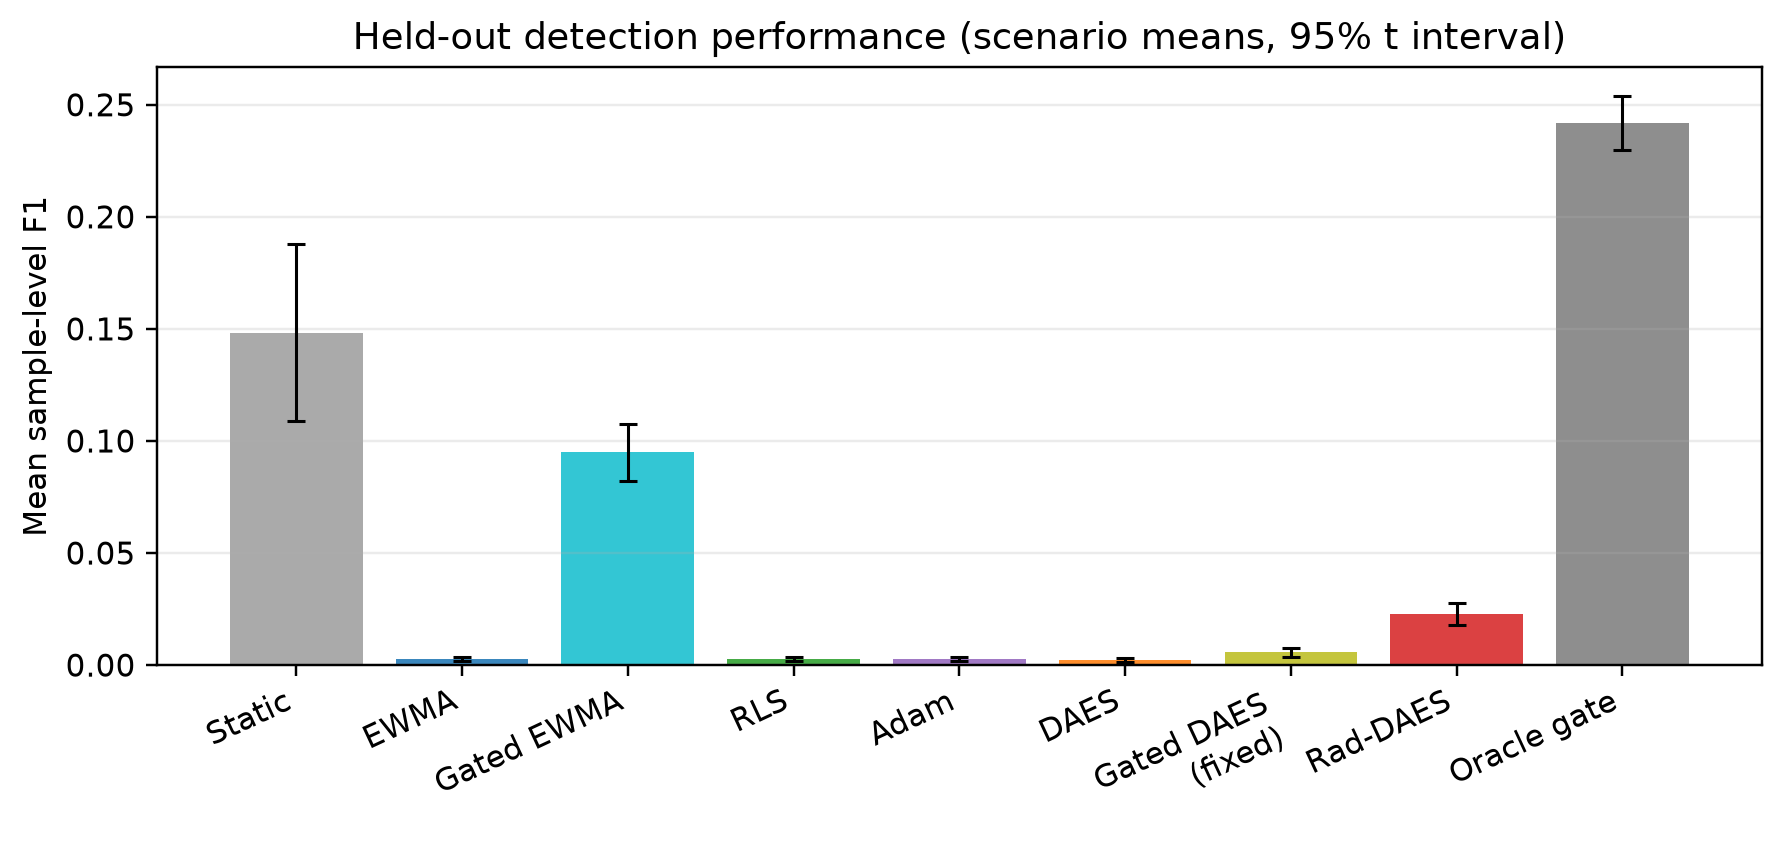
\includegraphics[width=0.92\linewidth]{../results/figures/fig_primary_f1.png}
\caption{Mean sample-level F1 by method. Error bars are 95\% Student-$t$ intervals across the 32 held-out scenario means. The oracle gate is a non-deployable reference.}
\label{fig:primary}
\end{figure}

\paragraph{The operating point dominates the ranking.}
The four methods whose development configurations satisfied the false-alarm constraint (EWMA, RLS, Adam, ungated DAES) have test F1 at most $0.003$ and detect at most 6\% of source events, with test FAR between 2.0 and 2.5/h. They are, in effect, blind at the calibrated operating point. The methods with visible detection either violate the false-alarm constraint or use labels: gated EWMA reaches F1 \GatedEWMAFone{} at \GatedEWMAFarPerHour{}/h, and Rad-DAES reaches \RadDAESFone{} at \RadDAESFarPerHour{}/h. \texttt{static} reaches \StaticFone{} only by alarming on 13.4\% of all samples. There is no deployable method in the matrix that is both sensitive and quiet. Figure~\ref{fig:tradeoff} plots this trade-off directly.

Table~\ref{tab:discrimination} separates threshold choice from separability. The oracle gate has the highest ROC AUC (0.773) and PR AUC (0.223), followed by \texttt{static} (0.728 and 0.128) and gated EWMA (0.691 and 0.089). Rad-DAES obtains ROC AUC \RadDAESRocAuc{} and PR AUC \RadDAESPrAuc{}, below both gated EWMA and \texttt{static}. The ordering is therefore not an artefact of one threshold: the DAES-based methods rank source samples less well than the simpler alternatives on these streams.

\begin{table}[t]
\centering
\caption{Threshold-free discrimination and gate behaviour. ROC/PR AUC use the pre-update score and do not depend on the alarm threshold. Event detection is the fraction of 960 source events with at least one alarm. Alarm fraction is the fraction of all evaluated samples that alarm. Release rate is the fraction of samples in which the sustained-exceedance release is active.}
\label{tab:discrimination}
\scriptsize
\setlength{\tabcolsep}{3pt}
\input{../results/tables/table_discrimination.tex}
\end{table}

\begin{figure}[t]
\centering
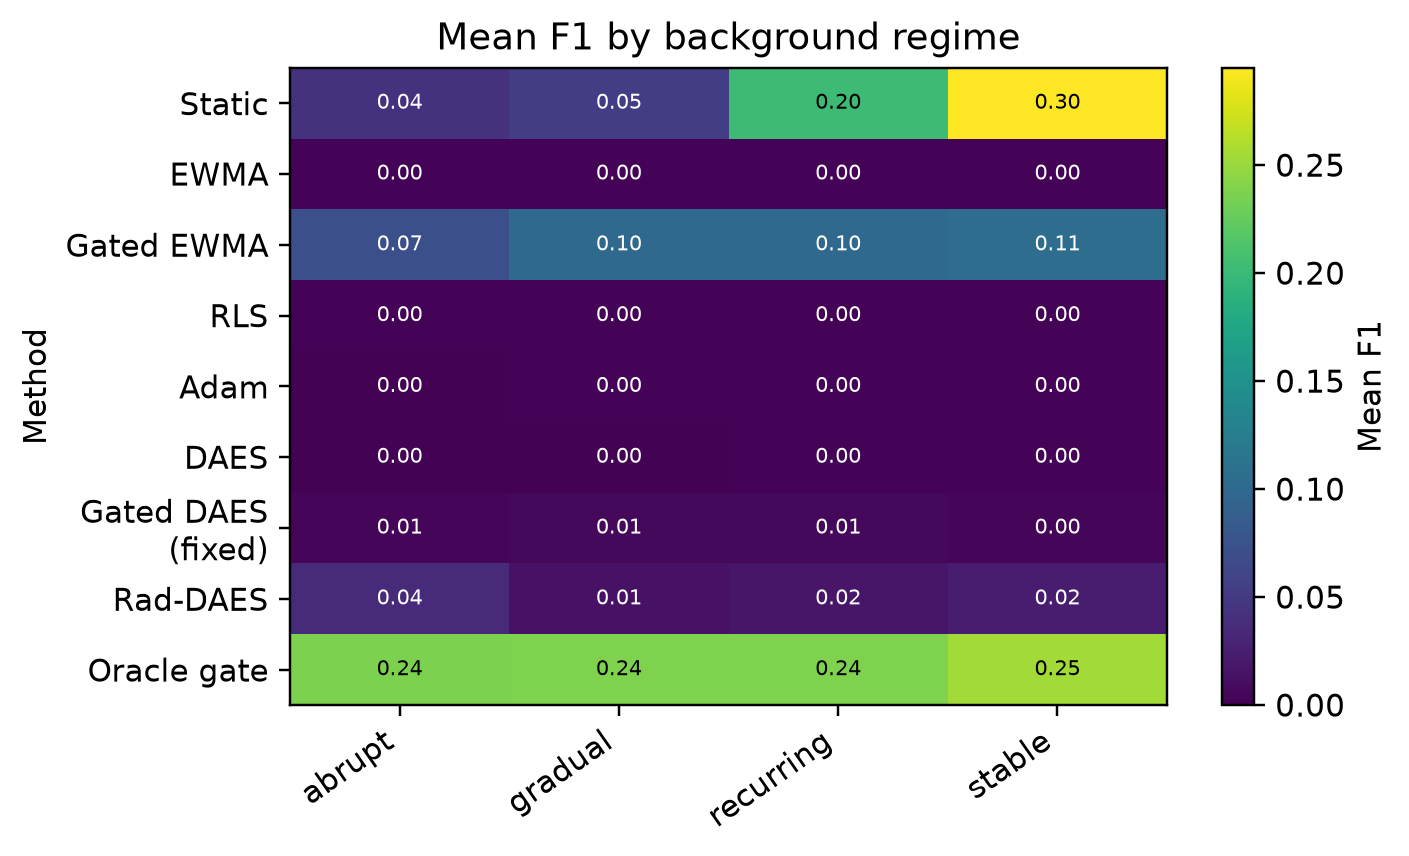
\includegraphics[width=0.92\linewidth]{../results/figures/fig_f1_by_regime.png}
\caption{Mean F1 by background regime. Each cell is the mean over the eight fault conditions and five seeds.}
\label{fig:regime}
\end{figure}

\begin{figure}[t]
\centering
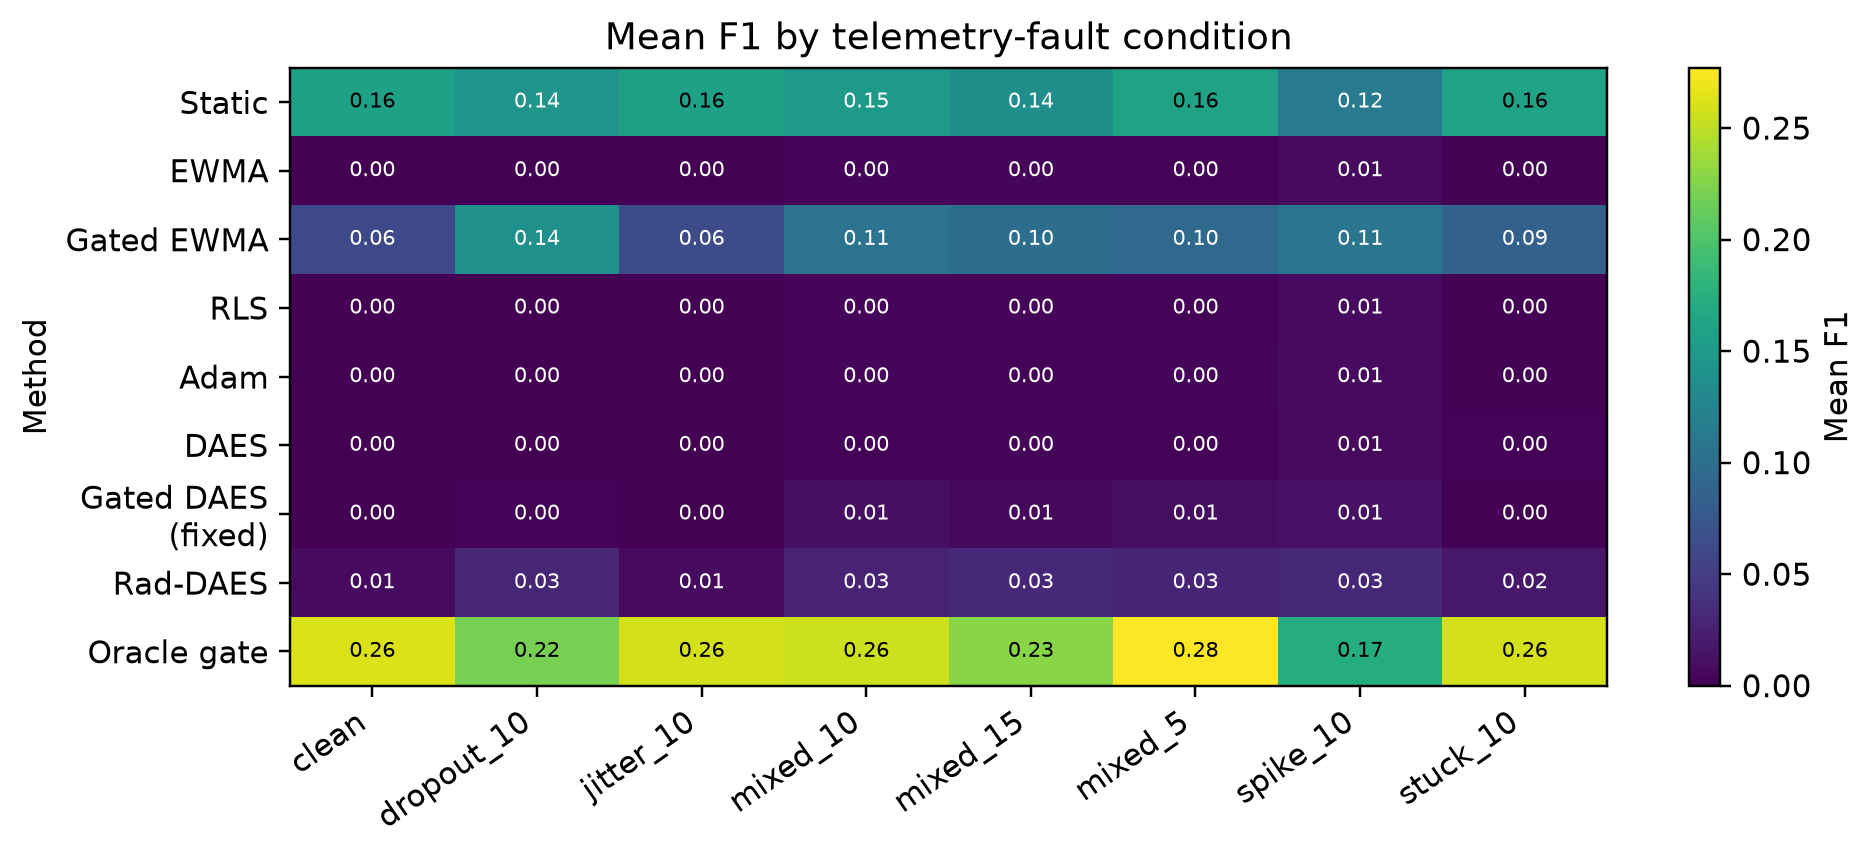
\includegraphics[width=0.98\linewidth]{../results/figures/fig_f1_by_fault.png}
\caption{Mean F1 by telemetry-fault condition. Each cell is the mean over the four regimes and five seeds.}
\label{fig:fault}
\end{figure}

\begin{figure}[t]
\centering
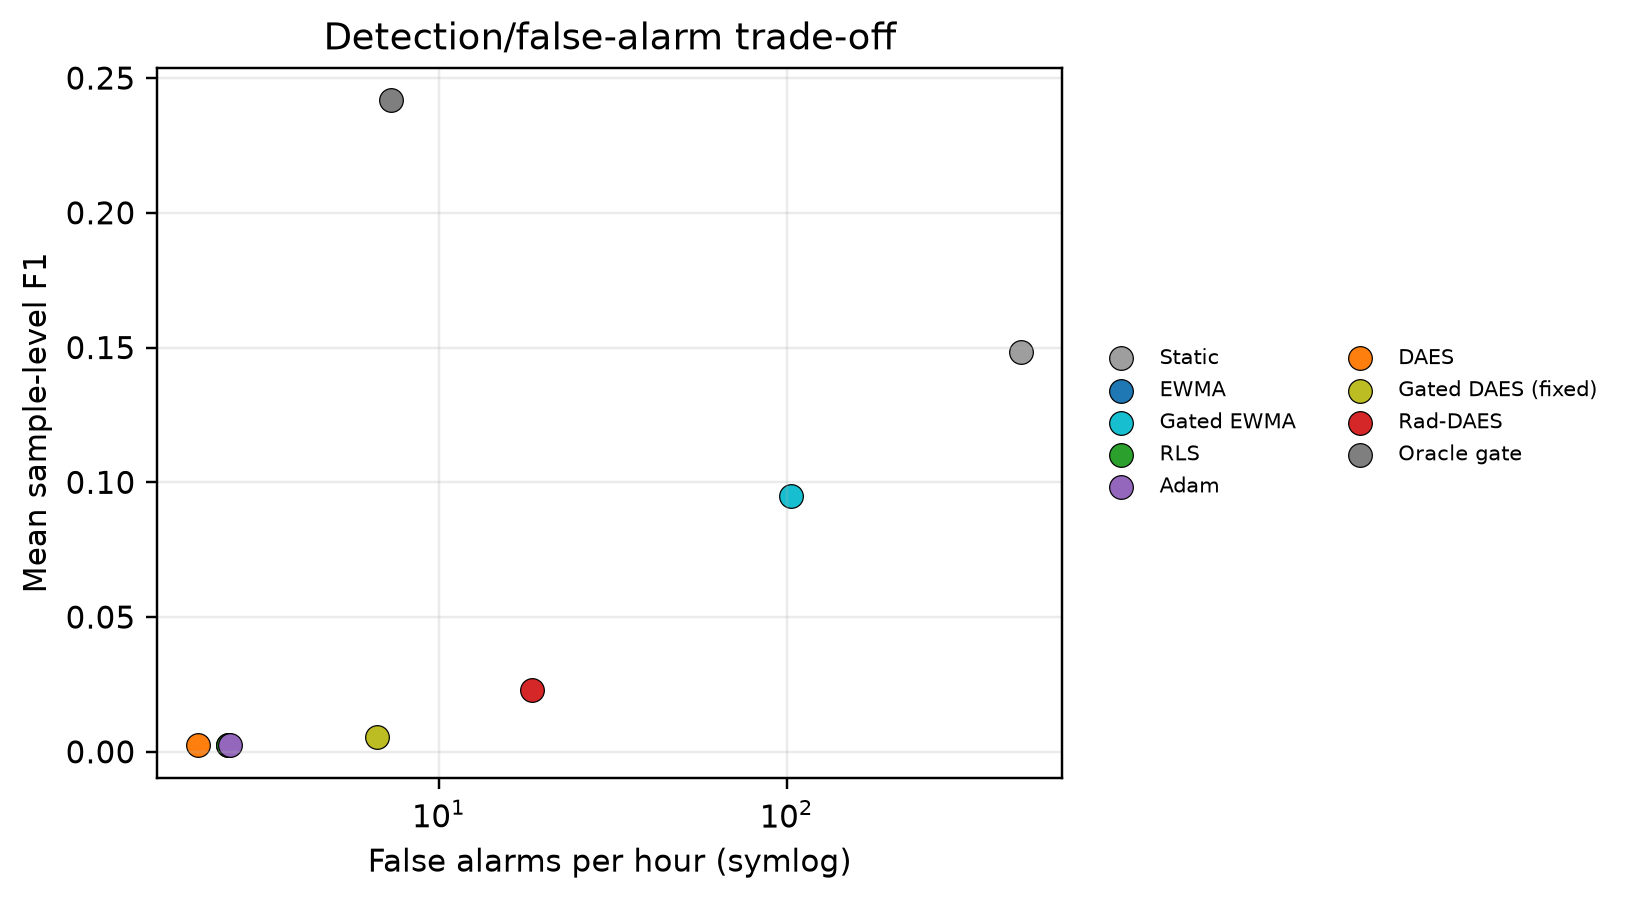
\includegraphics[width=0.78\linewidth]{../results/figures/fig_far_vs_f1.png}
\caption{Detection/false-alarm trade-off. The horizontal axis is symlog because static and some gated configurations produce very large drift-induced false-alarm burdens.}
\label{fig:tradeoff}
\end{figure}

\paragraph{Regime and fault structure.}
Figures~\ref{fig:regime} and~\ref{fig:fault} show that performance is not uniform. The recurring regime is the only regime not used for tuning; it is therefore the clearest check of whether a configuration generalises to a different drift shape. It does not rescue the candidate: Rad-DAES remains below gated EWMA and far below the oracle. Fault conditions change which samples are eligible for updating, so a method that looks adequate on clean streams can lose when dropout, jitter, stuck, or spike faults are present. The spike condition is the worst for false alarms: Rad-DAES reaches \RadDAESFarPerHour{}/h on average but 68.8/h under \texttt{spike\_10}, because a spike both alarms and freezes the update.

\paragraph{Gate behaviour.}
The gate rejects 26.1\% of clean samples and 33.8\% of source samples for Rad-DAES, and the sustained release is active on about $3\times10^{-6}$ of samples. The release is not merely rare: in the representative trace (Figure~\ref{fig:trace}) the consecutive-exceedance counter reaches 89 samples and then resets, one sample short of the 90-sample patience, so the model stays frozen through the step. The tracked mean remains near its pre-step value for roughly 350\,s while the true background has already moved by about 170 counts/s. The gate's source-rejection rate is the expected cost of protecting the background, but here the same mechanism also protects the background from the drift it is supposed to follow. Figure~\ref{fig:gate} summarises the rejection rates by sample type.

\begin{figure}[t]
\centering
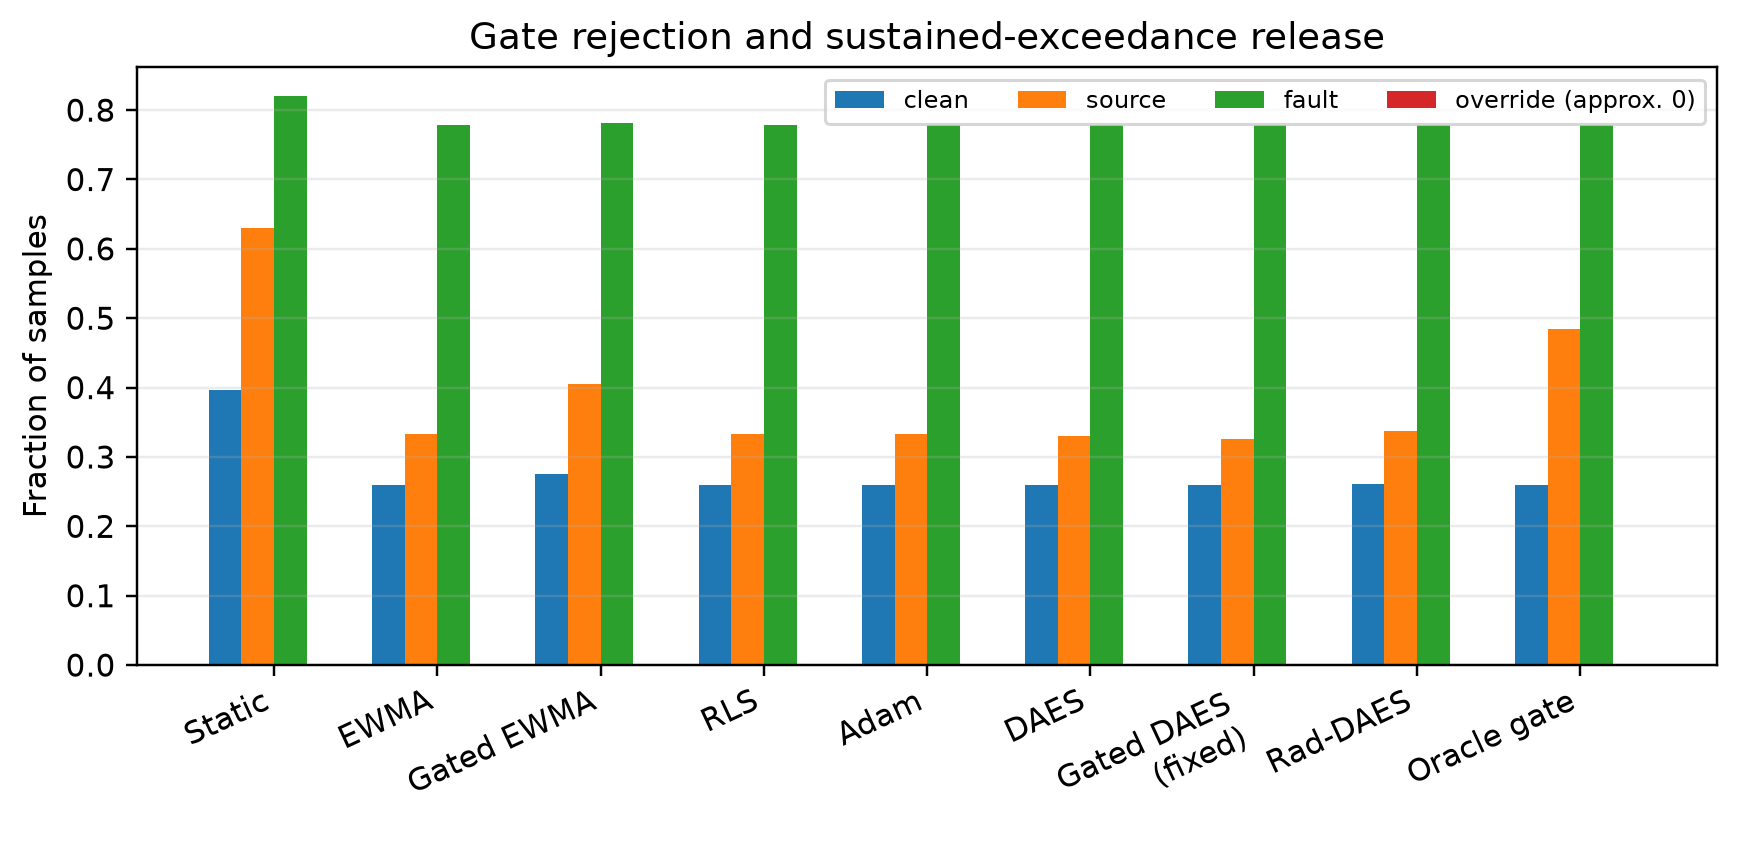
\includegraphics[width=0.92\linewidth]{../results/figures/fig_gate.png}
\caption{Gate rejection rates for clean, source, and fault samples, and the rate of sustained-exceedance release. A high source-rejection rate is the expected cost of protecting the background; it is also a recall risk.}
\label{fig:gate}
\end{figure}

\begin{figure}[t]
\centering
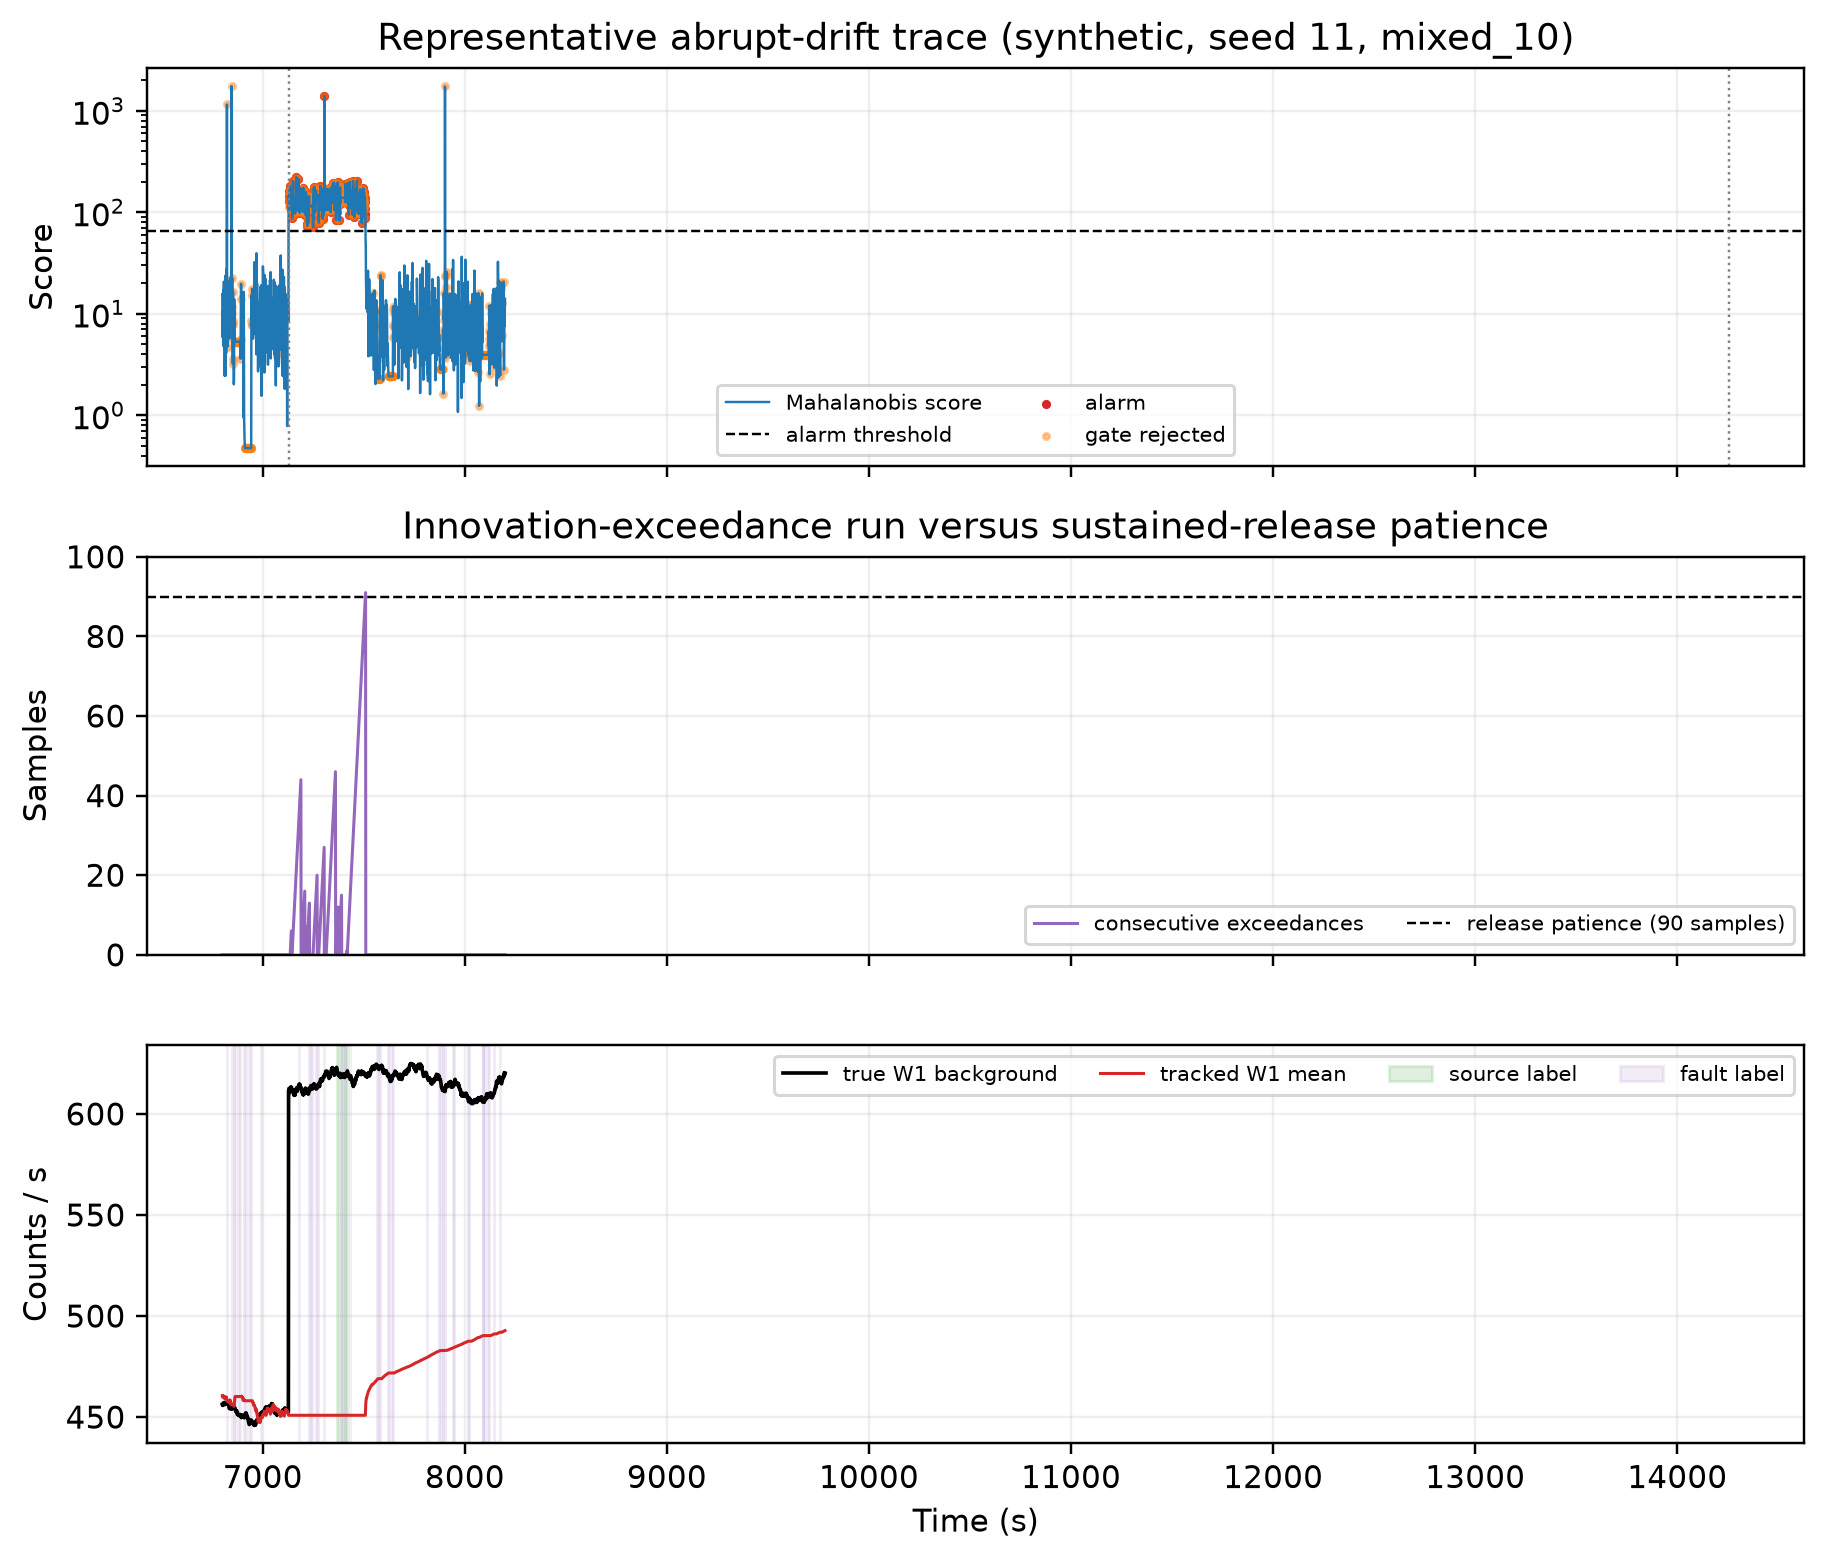
\includegraphics[width=0.95\linewidth]{../results/figures/fig_trace.png}
\caption{Representative abrupt-drift trace for Rad-DAES (synthetic, seed 11, \texttt{mixed\_10}). Top: pre-update score, alarms, and gate rejections. Middle: consecutive innovation exceedances versus the 90-sample release patience; the counter peaks at 89 and resets. Bottom: true and tracked W1 background, with source and fault labels.}
\label{fig:trace}
\end{figure}

\paragraph{Recovery and stability.}
Figure~\ref{fig:recovery} reports recovery time after abrupt steps. Recovery is defined as the first sample at which every window's relative mean error stays below 5\% for 30 consecutive samples; an event that never meets the condition is not silently counted as a success. Rad-DAES recovers 55 of 80 abrupt-step events with a mean recovery time of \RadDAESRecoveryMean{}\,s; gated EWMA recovers all 80 at \GatedEWMARecoveryMean{}\,s but with a much higher false-alarm burden; ungated EWMA and RLS recover all 80 at about 399\,s while remaining nearly blind to sources; \texttt{static} recovers none. Recovery and detection therefore pull in opposite directions in this matrix, and no method achieves both.

\begin{figure}[t]
\centering
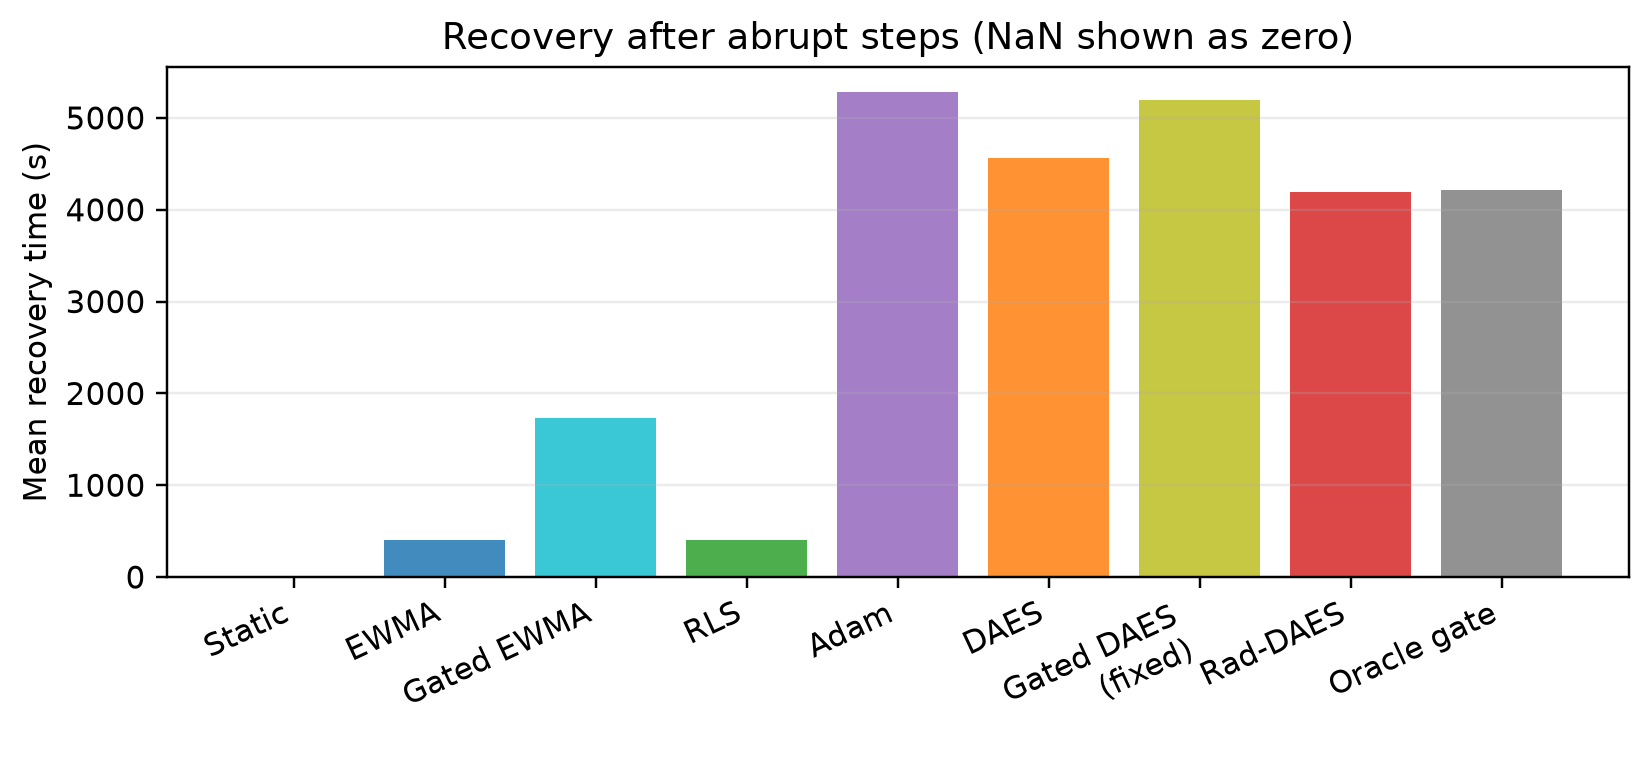
\includegraphics[width=0.78\linewidth]{../results/figures/fig_recovery.png}
\caption{Mean recovery time after abrupt steps. Missing values are shown as zero only for display; they are not treated as recovered in the tables.}
\label{fig:recovery}
\end{figure}

\begin{table}[t]
\centering
\caption{Paired differences (Rad-DAES minus the named method) over matched scenario/seed pairs. Each pair is one held-out run; the 160 pairs are 32 scenarios $\times$ 5 seeds, and the five seeds of a scenario are treated as independent observations, so within-scenario clustering is not modelled. Positive F1 is better; positive FAR and BG are worse. Intervals are descriptive 95\% Student-$t$ intervals and are not multiplicity-corrected.}
\label{tab:paired}
\scriptsize
\input{../results/tables/table_paired.tex}
\end{table}

\paragraph{Tuning and fallbacks.}
Table~\ref{tab:tuning} records the selected development configuration for each method. Four of the nine methods used a fallback, meaning that no candidate met both the background-error and false-alarm constraints on the development scenarios. Rad-DAES selected the largest gain in the grid ($\gamma=0.5$) with a development FAR of 28.6/h, more than fourteen times the constraint; gated EWMA selected the smallest EWMA weight but still had a development FAR of 99.4/h. The oracle gate selected the smallest gain ($\gamma=0.05$) and had a development FAR of 12.5/h. The oracle's advantage is therefore not an isolated gate effect: it combines perfect labelling with a ten-fold gentler step, and the two cannot be separated in this matrix. The selected configurations were frozen before the test matrix.

\begin{table}[t]
\centering
\caption{Selected development configurations and development means. ``Fallback'' means no candidate satisfied both the background-error and false-alarm constraints.}
\label{tab:tuning}
\scriptsize
\input{../results/tables/table_tuning.tex}
\end{table}

\section{Discussion}

The experiment was designed to test a trade-off, not to demonstrate that a new method wins. The answer is negative, and three mechanisms explain most of it.

\emph{First, the innovation guard confuses drift with a source.} A persistent background step produces a sustained score above the gate threshold, so the gate freezes the mean precisely when the mean needs to move. The 90-sample release was intended to break this deadlock, but it requires an uninterrupted run of exceedances; Poisson noise and the oscillating score reset the counter. In the representative trace the counter peaks at 89 and resets. The result is a frozen model, a long alarm burst, and a slow recovery. This is a design failure of the release rule, not a tuning issue: the rule is brittle by construction because it depends on a run length in a noisy sequence.

\emph{Second, the adaptive background appears to absorb source energy.} Both the mean and the covariance update on a 50-sample time constant, comparable to the 20--60\,s source duration. During the ramp of a source event the score is still below the gate threshold, so the gate passes those samples; the mean then moves toward the source and the covariance learns its outer product, and the score for the peak falls. This is consistent with the threshold-free results: \texttt{static}, which updates neither the mean nor the covariance, has ROC AUC 0.728, while the adaptive methods have ROC AUC between 0.558 and 0.691. We did not run a covariance-frozen or mean-frozen ablation, so the two channels are not separated experimentally; the static-versus-adaptive contrast supports the general mechanism, not the share attributable to covariance. It is the most plausible explanation for why the ungated methods detect only about 6\% of events despite a nominal 3--8$\sigma$ source amplitude.

\emph{Third, the selection rule was infeasible.} The development constraint (FAR $\le 2$/h, background error $\le 0.10$) could not be met by any gated configuration under abrupt drift. The fallback rule then chose configurations that violated the FAR constraint by one to two orders of magnitude, and those configurations were frozen for test. The four feasible methods were feasible only because they were nearly blind. The protocol therefore did not compare methods at a common, achievable operating point; it compared blind methods against noisy ones. A matched-FAR evaluation, or a prespecified ROC/PR analysis, would have been more informative. The ROC/PR table is reported here as a secondary analysis, but it was not the basis of the selection rule.

The practical implication is that the three decisions should not share one score. A drift detector, a source detector, and a telemetry-integrity check answer different questions \citep{gama2014survey,isermann2005model}; using the same Mahalanobis score for gating and alarming creates the coupling observed here. A two-timescale covariance (fast for the mean, slow or robust for the detector), or a covariance that is frozen during suspected sources, is a concrete next step. None of these is implemented or validated in this draft.

The draft does not establish that Rad-DAES is novel. The literature review here is structured but not a full systematic review; the closest related work on portal data and concept drift is cited only to frame the problem. A novelty claim would require a protocol-driven review and a direct comparison on public data.

\section{Limitations and threats to validity}

\begin{itemize}
  \item \textbf{No real data.} RADAI requires an account and a large download; PyRIID requires a compatible Python environment and spectra conversion; the JRC reference spectra are not a continuous portal stream. No credentials were used and no real stream was parsed. Gate~1 of the project plan is a partial failure.
  \item \textbf{Synthetic generator.} The regimes, source templates, amplitudes, and fault rates are design choices. They are not fitted to measured background. The Poisson model ignores detector resolution, dead time, and spectrum unfolding \citep{knoll2010radiation}. The $\sin^2$ source profile makes the peak narrow, which penalises sample-level F1; event-level detection is reported to reduce that sensitivity, but it does not eliminate it. The design is reported in the form recommended for simulation studies \citep{morris2019simulation}, but a synthetic study cannot substitute for measured streams.
  \item \textbf{Mechanism inferred, not isolated.} The adaptive-background explanation (mean and covariance) is supported by the static-versus-adaptive contrast and by the saved traces, but no covariance-frozen or mean-frozen ablation was run, so the two channels are not separated. The gate-deadlock explanation is directly visible in one representative trace; the 89-versus-90 near miss is illustrative, not a distributional estimate.
  \item \textbf{Small seed budget.} Five seeds were evaluated per scenario. The primary 95\% confidence intervals are calculated across the 32 scenario means after averaging the five seeds within each scenario. These intervals are descriptive and conditional on the fixed scenario design. They do not quantify uncertainty beyond the selected scenarios or account for model misspecification \citep{greenland2016statistical}.
  \item \textbf{No multiplicity correction.} The scenario-level and paired comparisons are descriptive. A claim of statistical significance is not made, and no false-discovery-rate procedure is applied \citep{benjamini1995controlling}.
  \item \textbf{Design choices.} The 90-sample (90\,s) release, the 0.5--1.5\,s timing bound, the 0.25--3.5 Fano bounds, the 0.25 covariance floor, the 50-sample covariance time constant, and the six windows are choices, not validated constants. Sensitivity analyses are future work.
  \item \textbf{Threshold transfer.} Thresholds calibrated on clean stable streams do not transfer to drift regimes: even the oracle gate has 7.3 false alarms/h on test. The 1/h calibration target is therefore not an operational guarantee, and portal false-alarm testing requires a broader operating-characteristic study than the one reported here \citep{burr2007alarm,leber2020false}.
  \item \textbf{DAES provenance.} The DAES equations follow the supplied scalar reference implementation. The matrix update in some generated planning material is not implemented as DAES. The wrapper's use of a Gaussian quasi-likelihood Hessian is an adaptation, not a theorem.
  \item \textbf{No field readiness.} Runtime is offline Python on synthetic arrays. No hardware latency, network delay, calibration uncertainty, or regulatory requirement is modelled.
\end{itemize}

\section{Reproducibility}

{\sloppy
The repository is self-contained and separate from the unrelated projects that share the workspace. The synthetic generator, gate, DAES controller, background model, detector, runner, tests, scripts, raw CSV files, tables, and figures are included. The packaging follows the reproducibility principle that data, code, and the computational narrative should be inspectable together \citep{peng2011reproducible}. The main commands are:\par}
\begin{verbatim}
python -m pip install -e .
python -m pytest -q
python scripts/run_benchmarks.py --mode full --output results/raw
python scripts/aggregate_results.py
python scripts/make_figures.py
python scripts/audit_results.py
\end{verbatim}
The runner writes a manifest with Python and package versions, configuration hashes, seed lists, and run counts. Every table and figure is generated from saved CSV or trace files; no result is typed into the manuscript by hand. The audit script checks matrix completeness, the frozen selection and thresholds, a determinism spot-check of saved rows, config hashes, and the presence of every table, figure, and macro used here. The original DAES reference file was read from an external snapshot for interface documentation and was not vendored or modified. Its SHA-256 and the archive SHA-256 are recorded in \texttt{docs/daes\_interface.md}.

{\sloppy
The raw run was launched with \texttt{--output results} and then moved into \texttt{results/raw/} to match the layout read by the aggregation and audit scripts; the only edited field was the trace-path column of \texttt{trace\_index.csv}. This is documented in \texttt{results/raw/README.md}.\par}

\section{Conclusion}

This draft delivers a small, complete, reproducible synthetic study of guarded drift-aware background tracking, and its result is negative. Rad-DAES does not improve the detection/false-alarm trade-off on these streams: its F1 is \RadDAESFone{} at \RadDAESFarPerHour{}/h, while the four false-alarm-compliant methods are nearly blind and the non-deployable oracle reaches only \BestValue{}. The traces identify two concrete failure modes, gate-induced freezing under drift and apparent adaptive-background contamination during source ramps, and the development selection rule is shown to be infeasible at the prespecified operating point. The value of the draft is the auditable pipeline and the explicit evidence boundary, not a claim that the candidate method is ready for a portal.

\bibliographystyle{plainnat}
\bibliography{references}

\appendix
\section{Implementation map}

\begin{table}[htbp]
\centering
\caption{Where each component is implemented and tested. Package paths are relative to \texttt{src/rad\_daes/}; script, test, and report paths are relative to the repository root.}
\small
\setlength{\tabcolsep}{4pt}
\begin{tabular}{lll}
\toprule
Component & Source & Test \\
\midrule
Synthetic streams & \texttt{data/synthetic.py} & \texttt{tests/test\_synthetic.py} \\
Window definitions & \texttt{preprocessing/windows.py} & configuration checks \\
Background model & \texttt{background/model.py} & \texttt{tests/test\_background.py} \\
Telemetry gate & \texttt{telemetry/gate.py} & \texttt{tests/test\_gate.py} \\
DAES controller & \texttt{adaptation/daes.py} & \texttt{tests/test\_daes.py} \\
Detector & \texttt{detection/detector.py} & runner integration \\
Metrics & \texttt{evaluation/metrics.py} & \texttt{tests/test\_metrics.py} \\
Runner and calibration & \texttt{evaluation/runner.py} & \texttt{tests/test\_runner.py} \\
Aggregation & \texttt{scripts/aggregate\_results.py} & table checks \\
Audit & \texttt{scripts/audit\_results.py} & \texttt{results/audit\_report.md} \\
\bottomrule
\end{tabular}
\end{table}

\section{Protocol revisions}

The source-placement bug, the sustained-exceedance release, the covariance floor, and the midpoint source profile were fixed on 28 October 2026 before the held-out matrix was run. The revision log is in \texttt{docs/protocol.md}. No held-out result was inspected before these changes. After the frozen test matrix was complete, the threshold-free ROC/PR table and the event-level detection summary were added as secondary analyses; they are computed from columns already saved by the frozen run, and the primary estimand and selection rule were not changed.

\clearpage
\section{Artifact inventory}

Table~\ref{tab:artifacts} lists the paths a reader needs in order to inspect or rerun the study. Counts describe the working repository of 28 October 2026 and exclude Python caches and \LaTeX{} build byproducts; the submission mirror differs only in that the cover-letter DOCX sits at the bundle root, so its \texttt{paper/} directory has six files.

\begin{table}[htbp]
\centering
\caption{Frozen artifact inventory. File counts exclude \texttt{\_\_pycache\_\_} directories.}
\label{tab:artifacts}
\small
\setlength{\tabcolsep}{4pt}
\begin{tabular}{llr}
\toprule
Path & Contents & Files \\
\midrule
\texttt{src/rad\_daes/} & Generator, gate, DAES controller, model, detector, metrics, runner & 16 \\
\texttt{configs/} & Data, model, and experiment configuration & 3 \\
\texttt{tests/} & Unit and integration tests (44 passing) & 7 \\
\texttt{results/raw/} & Calibration, development, and test CSVs; manifest; 4 traces & 13 \\
\texttt{results/tables/} & CSV, \LaTeX{} tables, and generated macros & 16 \\
\texttt{results/figures/} & Seven PNG figures & 7 \\
\texttt{docs/} & Protocol, decisions, DAES interface, results summary, checklist & 8 \\
\texttt{paper/} & Manuscript source, PDF, cover letter, bibliography, supplementary note & 7 \\
\bottomrule
\end{tabular}
\end{table}

The primary test artifact is \texttt{results/raw/test\_runs.csv} (1{,}440 rows). The audit report is regenerated by \texttt{scripts/audit\_results.py} and records 22 checks. No real radiation data are included, because none were obtained (Section~6).

\end{document}
"
\providecommand{\PaperSize}{letterpaper}
\usepackage[\PaperSize,margin=1in]{geometry}
\usepackage{amsmath,amssymb}
\usepackage{booktabs}
\usepackage{graphicx}
\usepackage{siunitx}
\usepackage[hidelinks]{hyperref}
\usepackage[numbers,sort]{natbib}
\usepackage{xcolor}
\usepackage{caption}
\usepackage{subcaption}

\hypersetup{
  pdftitle={Guarded Drift-Aware Background Tracking for Synthetic Radiation-Portal Count Streams: A Reproducible Benchmark and a Negative Result},
  pdfauthor={Tripti Kumari, Chayan Ojha, Mriganko Dey, Ankita Polley},
  pdfsubject={B.Tech group project, Department of Computer Science and Engineering (AI \& ML), Narula Institute of Technology, Agarpara}
}

% Generated by scripts/aggregate_results.py. Do not edit by hand.
\newcommand{\StaticFone}{0.148}
\newcommand{\StaticFarPerHour}{472.4}
\newcommand{\StaticBgRelError}{0.055}
\newcommand{\StaticRecall}{0.370}
\newcommand{\StaticPrecision}{0.249}
\newcommand{\StaticRecoveryMean}{---}
\newcommand{\EWMAFone}{0.003}
\newcommand{\EWMAFarPerHour}{2.476}
\newcommand{\EWMABgRelError}{0.015}
\newcommand{\EWMARecall}{0.002}
\newcommand{\EWMAPrecision}{0.089}
\newcommand{\EWMARecoveryMean}{399.1}
\newcommand{\GatedEWMAFone}{0.095}
\newcommand{\GatedEWMAFarPerHour}{102.7}
\newcommand{\GatedEWMABgRelError}{0.017}
\newcommand{\GatedEWMARecall}{0.121}
\newcommand{\GatedEWMAPrecision}{0.473}
\newcommand{\GatedEWMARecoveryMean}{1734}
\newcommand{\RLSFone}{0.003}
\newcommand{\RLSFarPerHour}{2.476}
\newcommand{\RLSBgRelError}{0.015}
\newcommand{\RLSRecall}{0.002}
\newcommand{\RLSPrecision}{0.089}
\newcommand{\RLSRecoveryMean}{399.1}
\newcommand{\AdamFone}{0.003}
\newcommand{\AdamFarPerHour}{2.500}
\newcommand{\AdamBgRelError}{0.028}
\newcommand{\AdamRecall}{0.002}
\newcommand{\AdamPrecision}{0.078}
\newcommand{\AdamRecoveryMean}{5286}
\newcommand{\DAESFone}{0.002}
\newcommand{\DAESFarPerHour}{2.031}
\newcommand{\DAESBgRelError}{0.038}
\newcommand{\DAESRecall}{0.001}
\newcommand{\DAESPrecision}{0.054}
\newcommand{\DAESRecoveryMean}{4564}
\newcommand{\GatedDAESFixedFone}{0.006}
\newcommand{\GatedDAESFixedFarPerHour}{6.649}
\newcommand{\GatedDAESFixedBgRelError}{0.069}
\newcommand{\GatedDAESFixedRecall}{0.004}
\newcommand{\GatedDAESFixedPrecision}{0.054}
\newcommand{\GatedDAESFixedRecoveryMean}{5196}
\newcommand{\RadDAESFone}{0.023}
\newcommand{\RadDAESFarPerHour}{18.508}
\newcommand{\RadDAESBgRelError}{0.025}
\newcommand{\RadDAESRecall}{0.024}
\newcommand{\RadDAESPrecision}{0.142}
\newcommand{\RadDAESRecoveryMean}{4198}
\newcommand{\OracleGateFone}{0.242}
\newcommand{\OracleGateFarPerHour}{7.292}
\newcommand{\OracleGateBgRelError}{0.014}
\newcommand{\OracleGateRecall}{0.158}
\newcommand{\OracleGatePrecision}{0.721}
\newcommand{\OracleGateRecoveryMean}{4213}
\newcommand{\BestMethod}{Oracle gate}
\newcommand{\BestValue}{0.242}
\newcommand{\NScenarios}{32}
\newcommand{\StaticRocAuc}{0.728}
\newcommand{\StaticPrAuc}{0.128}
\newcommand{\StaticEventDetection}{0.821}
\newcommand{\StaticAlarmFraction}{0.134}
\newcommand{\StaticGateRejectClean}{0.397}
\newcommand{\StaticGateRejectSource}{0.630}
\newcommand{\StaticGateOverrideRate}{0.002}
\newcommand{\EWMARocAuc}{0.622}
\newcommand{\EWMAPrAuc}{0.031}
\newcommand{\EWMAEventDetection}{0.060}
\newcommand{\EWMAAlarmFraction}{0.001}
\newcommand{\EWMAGateRejectClean}{0.260}
\newcommand{\EWMAGateRejectSource}{0.333}
\newcommand{\EWMAGateOverrideRate}{0.000}
\newcommand{\GatedEWMARocAuc}{0.691}
\newcommand{\GatedEWMAPrAuc}{0.089}
\newcommand{\GatedEWMAEventDetection}{0.406}
\newcommand{\GatedEWMAAlarmFraction}{0.030}
\newcommand{\GatedEWMAGateRejectClean}{0.275}
\newcommand{\GatedEWMAGateRejectSource}{0.406}
\newcommand{\GatedEWMAGateOverrideRate}{0.000}
\newcommand{\RLSRocAuc}{0.622}
\newcommand{\RLSPrAuc}{0.031}
\newcommand{\RLSEventDetection}{0.060}
\newcommand{\RLSAlarmFraction}{0.001}
\newcommand{\RLSGateRejectClean}{0.260}
\newcommand{\RLSGateRejectSource}{0.333}
\newcommand{\RLSGateOverrideRate}{0.000}
\newcommand{\AdamRocAuc}{0.637}
\newcommand{\AdamPrAuc}{0.033}
\newcommand{\AdamEventDetection}{0.056}
\newcommand{\AdamAlarmFraction}{0.001}
\newcommand{\AdamGateRejectClean}{0.260}
\newcommand{\AdamGateRejectSource}{0.333}
\newcommand{\AdamGateOverrideRate}{0.000}
\newcommand{\DAESRocAuc}{0.600}
\newcommand{\DAESPrAuc}{0.024}
\newcommand{\DAESEventDetection}{0.054}
\newcommand{\DAESAlarmFraction}{0.001}
\newcommand{\DAESGateRejectClean}{0.260}
\newcommand{\DAESGateRejectSource}{0.330}
\newcommand{\DAESGateOverrideRate}{0.000}
\newcommand{\GatedDAESFixedRocAuc}{0.558}
\newcommand{\GatedDAESFixedPrAuc}{0.019}
\newcommand{\GatedDAESFixedEventDetection}{0.059}
\newcommand{\GatedDAESFixedAlarmFraction}{0.002}
\newcommand{\GatedDAESFixedGateRejectClean}{0.260}
\newcommand{\GatedDAESFixedGateRejectSource}{0.326}
\newcommand{\GatedDAESFixedGateOverrideRate}{0.000}
\newcommand{\RadDAESRocAuc}{0.629}
\newcommand{\RadDAESPrAuc}{0.036}
\newcommand{\RadDAESEventDetection}{0.105}
\newcommand{\RadDAESAlarmFraction}{0.005}
\newcommand{\RadDAESGateRejectClean}{0.261}
\newcommand{\RadDAESGateRejectSource}{0.338}
\newcommand{\RadDAESGateOverrideRate}{0.000}
\newcommand{\OracleGateRocAuc}{0.773}
\newcommand{\OracleGatePrAuc}{0.223}
\newcommand{\OracleGateEventDetection}{0.736}
\newcommand{\OracleGateAlarmFraction}{0.004}
\newcommand{\OracleGateGateRejectClean}{0.260}
\newcommand{\OracleGateGateRejectSource}{0.485}
\newcommand{\OracleGateGateOverrideRate}{0.000}
\newcommand{\PairedStaticFone}{-0.125}
\newcommand{\PairedStaticFarPerHour}{-453.9}
\newcommand{\PairedStaticBgRelError}{-0.029}
\newcommand{\PairedEWMAFone}{0.020}
\newcommand{\PairedEWMAFarPerHour}{16.032}
\newcommand{\PairedEWMABgRelError}{0.010}
\newcommand{\PairedGatedEWMAFone}{-0.072}
\newcommand{\PairedGatedEWMAFarPerHour}{-84.240}
\newcommand{\PairedGatedEWMABgRelError}{0.008}
\newcommand{\PairedRLSFone}{0.020}
\newcommand{\PairedRLSFarPerHour}{16.032}
\newcommand{\PairedRLSBgRelError}{0.010}
\newcommand{\PairedAdamFone}{0.020}
\newcommand{\PairedAdamFarPerHour}{16.008}
\newcommand{\PairedAdamBgRelError}{-0.002}
\newcommand{\PairedDAESFone}{0.020}
\newcommand{\PairedDAESFarPerHour}{16.478}
\newcommand{\PairedDAESBgRelError}{-0.012}
\newcommand{\PairedGatedDAESFixedFone}{0.017}
\newcommand{\PairedGatedDAESFixedFarPerHour}{11.860}
\newcommand{\PairedGatedDAESFixedBgRelError}{-0.043}
\newcommand{\PairedOracleGateFone}{-0.219}
\newcommand{\PairedOracleGateFarPerHour}{11.217}
\newcommand{\PairedOracleGateBgRelError}{0.011}


\title{Guarded Drift-Aware Background Tracking for Synthetic Radiation-Portal Count Streams:\\A Reproducible Benchmark and a Negative Result}
\author{%
  Tripti Kumari\\
  Chayan Ojha\\
  Mriganko Dey\\
  Ankita Polley\\[0.8em]
  \small Department of Computer Science and Engineering (AI \& ML)\\
  \small Narula Institute of Technology, Agarpara, West Bengal\\
  \small B.Tech in Computer Science and Engineering (Artificial Intelligence and Machine Learning)\\
  \small Academic year 2026--2027 (provisional)
}
\date{28 October 2026}

\begin{document}
\maketitle

\begin{abstract}
Radiation-portal monitors must separate source-like count excursions from a drifting background and from telemetry faults. This draft evaluates \emph{Rad-DAES}, a candidate pipeline that combines a four-condition telemetry-integrity gate, a pre-update Mahalanobis detector, and the scalar drift-aware step size of the supplied DAES reference implementation. The study is synthetic-only and deliberately narrow: six-window Poisson streams under four background regimes and eight telemetry-fault conditions, tuned on development seeds only, with the recurring regime held out, and evaluated on \NScenarios{} scenarios with five seeds and nine methods (1{,}440 runs). The result is negative. No deployable method achieved both useful event detection and an acceptable false-alarm rate. The best mean sample-level F1 is \BestValue{} for the non-deployable oracle gate; Rad-DAES obtains \RadDAESFone{} with \RadDAESFarPerHour{} false alarms per hour, and the four methods whose development configurations met the false-alarm constraint obtain F1 at most $0.003$ and detect at most 6\% of source events. The traces show why: after an abrupt background step the innovation guard freezes the model for hundreds of seconds, the 90-sample sustained-release rule almost never fires for Rad-DAES (below 0.01\% of its samples), and the saved traces and static-versus-adaptive comparison are consistent with the adaptive background absorbing source energy during event ramps, although this mechanism was not isolated experimentally. These are simulation results from an unvalidated generator. They do not establish field readiness, operational safety, or novelty, and no statistical-significance claim is made.
\end{abstract}

\section{Introduction}

A radiation portal monitor observes a stream of gamma counts in several energy windows \citep{knoll2010radiation,runkle2009photon}. A source that passes through the portal raises some windows for a short interval; background radon, weather, cargo, and detector drift change the same windows over minutes or hours \citep{sim2021background,sim2024cargo}; and a telemetry fault can make an observation invalid, late, stuck, or implausibly dispersed \citep{isermann2005model,little2019missing}. A background tracker that adapts too eagerly can absorb the source it is meant to detect. A tracker that adapts too slowly leaves a drift-induced residual that looks like a source. The engineering problem is therefore a coupling between detection, adaptation, and data quality, not a standalone optimizer problem.

This draft asks a narrow question: under matched synthetic streams, does a guarded DAES pipeline improve the detection/false-alarm/stability trade-off relative to static, EWMA, gated EWMA, RLS, Adam, ungated DAES, fixed-step gated DAES, and an oracle gate? The answer reported here is no, and the more useful output is a reproducible account of why. The DAES component is the original scalar step-size heuristic supplied with the project brief. The matrix update that appears in some generated planning material is explicitly not implemented as DAES; the discrepancy is documented in the repository.

The paper makes four bounded contributions:
\begin{enumerate}
  \item a reproducible synthetic benchmark with labelled background regimes, source events, and telemetry faults, including a held-out recurring regime;
  \item a documented separation between the original DAES scalar controller, the Gaussian quasi-likelihood curvature used by the wrapper, and the telemetry gate;
  \item a complete negative-and-mixed report: all methods and scenarios are reported, including the cases where the candidate loses;
  \item a mechanistic account, supported by saved per-step traces, of two failure modes: gate-induced freezing under drift and apparent adaptive-background contamination during source ramps.
\end{enumerate}

No real radiation data are used. The data-access blockers are recorded in the repository. The experiments are a first draft, not a field validation.

\section{Related work}

\paragraph{Background estimation and source detection.}
Radiation-portal analysis has moved toward large, realistic datasets and reproducible algorithm development \citep{ghawaly2020data,ghawaly2026radai}. Detection methods range from moving-source algorithms over portal networks \citep{coulon2014moving} to studies of cargo-induced background suppression \citep{sim2024cargo}, standardised portal controls and readouts \citep{tinker2010standardisation}, and standardised data formats \citep{bae2025format}. Reviews of portal detection technology emphasise the low signal-to-background regime and the operational cost of nuisance alarms \citep{runkle2009photon}, while Monte Carlo studies show that background composition and shielding change the observed count distribution \citep{sim2021background}. These works motivate the six-window count representation and the concern with background drift, but they do not provide a local stream on which the present pipeline can be validated. The synthetic generator is therefore an explicit placeholder.

\paragraph{Drift, smoothing, and change detection.}
Concept-drift adaptation distinguishes transient noise, gradual change, abrupt change, and recurring change \citep{gama2014survey}. Non-stationary time-series models make the same point formally: a process whose parameters change over time cannot be summarised by a single stationary model \citep{dahlhaus1997fitting}. The EWMA control chart \citep{roberts1959control}, its broader exponential-smoothing formulation \citep{gardner1985exponential}, and the CUSUM procedure \citep{page1954continuous} are classical tools for the same problem. The gate in this draft uses a sliding-window dispersion check and an innovation threshold rather than a full CUSUM, but the design tension is the same: a persistent shift should eventually be tracked, while a short source-like excursion should not contaminate the background.

\paragraph{Multivariate anomaly detection.}
The Mahalanobis distance provides a scale-free multivariate score that accounts for covariance \citep{mahalanobis1936distance}, and anomaly-detection surveys place covariance-based scoring among the classical statistical approaches \citep{chandola2009anomaly}. The detector in this draft uses that score on a pre-update innovation, so the covariance estimate directly controls both sensitivity and the false-alarm rate. This is a modelling choice, not a claim that the synthetic streams satisfy the Gaussian assumptions under which the score is usually derived.

\paragraph{Detection thresholds and false alarms.}
The Neyman--Pearson criterion formalises the trade-off between detection probability and false-alarm probability \citep{neyman1933problem}. Radiation-portal practice treats alarm criteria and false-alarm testing as first-class design problems rather than afterthoughts \citep{burr2007alarm,leber2020false}, and ROC analysis is the standard way to report threshold-free discrimination \citep{fawcett2006roc}. These sources motivate the two reporting layers used here: a calibrated operating point for the primary comparison, and a threshold-free ROC/PR analysis as a secondary check.

\paragraph{Step sizes and robust estimation.}
Polyak-style gradient methods and two-point step-size rules provide the optimisation background for adaptive step sizes \citep{barzilai1988two,polyak1963gradient}. The supplied DAES implementation is a scalar heuristic in this family: it estimates the largest curvature eigenvalue with power iteration and scales the step by its inverse. Robust location estimation \citep{huber1964robust} and model-based fault diagnosis \citep{isermann2005model} motivate the separation between an outlier-resistant update and a fault detector. Adam \citep{kingma2015adam} and recursive least squares \citep{ljung1999system} are included as optimisation/estimation baselines, not as claims about radiation physics.

\section{Methods}

\subsection{Synthetic streams}

Each stream is a sequence of $D=6$ non-negative count vectors at 1\,Hz. The six energy windows and nominal count rates are design choices taken from the project brief, not calibrated detector properties. Counts are modelled as Poisson variates, the standard first-order description of counting statistics \citep{knoll2010radiation}. For window $j$ and time $t$,
\begin{equation}
  x_{t,j} \sim \mathrm{Poisson}\bigl(\mu^{\mathrm{true}}_{t,j} + s_{t,j}\bigr),
\end{equation}
where $\mu^{\mathrm{true}}_{t}$ is a labelled background mean and $s_{t}$ is a labelled source excess. Poisson draws are made after the background and source terms are combined. Telemetry faults are applied afterwards.

The background regimes are:
\begin{itemize}
  \item \texttt{stable}: a small AR(1) fluctuation around the nominal rate;
  \item \texttt{gradual}: a slow sinusoidal trend plus a linear trend;
  \item \texttt{abrupt}: two multiplicative step changes with different per-window factors;
  \item \texttt{recurring}: three broad bumps, strongest in the low- and high-energy windows.
\end{itemize}
The recurring regime is held out from tuning. Each 6\,h stream attempts six source events of 20--60\,s, with amplitudes 3--8 baseline standard deviations and three templates. The excess follows a $\sin^2$ profile, so a labelled event has low amplitude at both ends and a narrow peak. Fault conditions are \texttt{clean}, \texttt{mixed\_5}, \texttt{mixed\_10}, \texttt{mixed\_15}, and single-mode \texttt{dropout\_10}, \texttt{jitter\_10}, \texttt{stuck\_10}, and \texttt{spike\_10}; the suffix is the approximate fraction of affected samples. The generator, labels, and seeds are deterministic. The design follows the reporting principles for simulation studies: the data-generating mechanism, the tuning rule, and the evaluation estimands are fixed before the held-out matrix is examined \citep{morris2019simulation}.

\subsection{Background model and detector}

The background state is a mean $\mu_t$ and covariance $\Sigma_t$. Detection uses the pre-update innovation
\begin{equation}
  r_t = x_t - \mu_{t-1}, \qquad
  s_t = r_t^\top \bigl(\Sigma_{t-1} + \epsilon I\bigr)^{-1} r_t,
  \label{eq:score}
\end{equation}
with $\epsilon=10^{-6}$. The quadratic form is the Mahalanobis score \citep{mahalanobis1936distance}, used here as a multivariate monitoring statistic. An alarm requires two consecutive scores above a calibrated threshold $\tau_{\mathrm{alarm}}$. The detector never sees the updated background for the current sample: detection precedes adaptation. The detector is evaluated on every sample, including samples that the telemetry gate rejects for updating; a high score can therefore alarm and freeze the model at the same time.

The Gaussian quasi-likelihood
\begin{equation}
  L_t(\theta) = \tfrac12 (x_t-\theta)^\top \Sigma_{t-1}^{-1}(x_t-\theta)
\end{equation}
has gradient $-\Sigma_{t-1}^{-1}r_t$ and Hessian $H_t=\Sigma_{t-1}^{-1}$, the local quadratic model used by Gaussian state estimation \citep{ljung1999system}. The covariance is tracked separately. On an eligible sample, with post-update residual $u_t=x_t-\mu_t$,
\begin{align}
  \tilde\Sigma_t &= (1-\beta)\Sigma_{t-1} + \beta u_t u_t^\top,\\
  \Sigma_t &= (1-\rho)\tilde\Sigma_t + \rho\,\mathrm{diag}(\tilde\Sigma_t),\\
  \mathrm{diag}(\Sigma_t) &\leftarrow \max\!\bigl(\mathrm{diag}(\Sigma_t),\, \max(10^{-6}, 0.25\,\mu_0)\bigr),
\end{align}
with $\beta=0.02$, $\rho=0.10$, and $\mu_0$ the nominal count vector. Both updates are exponentially weighted averages, the recursive form used in exponential smoothing \citep{gardner1985exponential}. The diagonal floor is a regularisation choice; it is not a claim that the true covariance is Poisson. The covariance time constant is 50 samples, comparable to the 20--60\,s source duration, which is relevant to the results below.

\subsection{Telemetry-integrity gate}

The gate is a conjunction of four conditions evaluated on the raw observation and a length-10 sliding buffer. It separates data-quality screening from fault diagnosis: the conditions are domain-specific checks, not a general fault-diagnosis model \citep{isermann2005model}, and the dropout condition is a missing-data rule rather than an imputation method \citep{little2019missing}:
\begin{enumerate}
  \item \textbf{validity}: every channel is finite and strictly positive;
  \item \textbf{timing}: $0.5 \le \Delta t_t \le 1.5$\,s;
  \item \textbf{Poisson dispersion}: $0.25 \le \mathrm{Var}_W(x_j)/\mathrm{Mean}_W(x_j) \le 3.5$ in every window;
  \item \textbf{innovation}: $s_t \le \tau_{\mathrm{gate}}$, or a sustained-exceedance release is active.
\end{enumerate}
The release activates after 90 consecutive samples that pass validity, timing, and dispersion but exceed $\tau_{\mathrm{gate}}$, and resets on any other telemetry failure or on a score at or below threshold. The patience is longer than the longest synthetic source event (60\,s). It is a design choice added to prevent a persistent background step from freezing the mean and producing an unbounded false-alarm burst. The gate is separate from the detector: a sample can alarm and still be rejected for updating, and the evaluation reports both decisions.

\subsection{Original DAES controller}

The supplied DAES implementation is a scalar step-size heuristic for gradient descent on a drifting strongly convex quadratic. It estimates $\lambda_{\max}(H_t)$ by $k$ power iterations, computes the Rayleigh quotient $q_t$, and uses
\begin{align}
  d_t &= \frac{|q_t-q_{t-1}|}{\max(|q_{t-1}|,10^{-12})},\\
  \alpha_t &= \mathrm{clip}(\alpha_0+\kappa d_t,\alpha_0,\alpha_{\max}),\\
  \hat\lambda_t &= (1-\alpha_t)\hat\lambda_{t-1}+\alpha_t q_t,\\
  \eta_t &= \frac{\gamma}{(1+s)\hat\lambda_t},
\end{align}
with an upward correction $\hat\lambda_t\leftarrow\max(\hat\lambda_t,q_t)$ when $q_t>\hat\lambda_{t-1}$. The reference defaults are $\gamma=1.78$, $s=0.10$ (a fixed safety margin, distinct from the score $s_t$ in Eq.~\eqref{eq:score}), $k=7$, $\alpha_0=0.16$, $\alpha_{\max}=0.82$, and $\kappa=7.0$. Rad-DAES tunes $\gamma$ on development data; the equation form is unchanged.

\subsection{Rad-DAES wrapper and baselines}

When the gate passes, Rad-DAES applies
\begin{equation}
  \mu_t = \mu_{t-1} + \eta_t \Sigma_{t-1}^{-1} r_t,
\end{equation}
which is gradient descent on $L_t$ with the scalar DAES step. When the gate rejects, the mean and covariance are frozen. The baselines are:
\begin{itemize}
  \item \texttt{static}: initial mean and covariance frozen;
  \item \texttt{ewma}: fixed-$\alpha$ EWMA mean and the same covariance update;
  \item \texttt{gated\_ewma}: EWMA behind the gate;
  \item \texttt{rls}: recursive least squares with forgetting;
  \item \texttt{adam}: Adam on the Gaussian quasi-likelihood gradient;
  \item \texttt{daes}: ungated DAES;
  \item \texttt{gated\_daes\_fixed}: gate plus a DAES step frozen at initialisation;
  \item \texttt{oracle\_gate}: gate replaced by the true source/fault labels; non-deployable reference.
\end{itemize}
All methods share the detector, windows, covariance rule where applicable, and calibration procedure.

\subsection{Protocol and estimands}

The held-out matrix is $4$ regimes $\times$ $8$ fault conditions $\times$ $5$ seeds $=160$ streams; each stream is processed by nine methods, giving 1{,}440 runs. Development tuning uses five seeds, three regimes (\texttt{stable}, \texttt{gradual}, \texttt{abrupt}), and \texttt{mixed\_10} faults. The tuning grid contains 69 candidate configurations. For each method, the selected configuration maximises mean development F1 subject to mean background relative error $\le 0.10$ and mean false alarms per hour $\le 2.0$; if no candidate is feasible, the least-violating candidate is used and the fallback is reported. Four methods had a feasible candidate, four used the fallback rule, and \texttt{static} has no tunable parameter and is marked fixed.

Alarm thresholds are the empirical $1-1/3600$ quantile of pre-update scores on clean stable development streams, pooled over five seeds; the gate threshold is the 0.999 quantile with a floor of 10. Both are frozen before test. The calibration target follows portal practice for false-alarm testing \citep{burr2007alarm,leber2020false}. The primary estimand is mean sample-level F1 across the 32 test scenarios, each weighted equally. Secondary estimands are false alarms per hour over non-source time, background relative error on non-source/non-fault samples, event-level detection (the fraction of the 960 source events with at least one alarm), threshold-free ROC and PR AUC computed from the pre-update score \citep{fawcett2006roc}, recovery time after abrupt steps, detection latency, update stability, runtime, and gate rejection rates. Intervals are two-sided 95\% Student-$t$ intervals: primary intervals are computed across the 32 scenario means after averaging the five seeds within each scenario, and paired intervals in Table~\ref{tab:paired} are computed across matched scenario/seed runs. The paired calculation treats the five seeds of a scenario as independent, so within-scenario clustering is not modelled \citep{cameron2015cluster}. No multiplicity correction is applied \citep{benjamini1995controlling}, and the intervals are reported descriptively rather than as significance tests \citep{greenland2016statistical}.

\section{Results}

Table~\ref{tab:primary} reports the primary estimand and the main secondary outcomes. Rad-DAES obtains mean F1 \RadDAESFone{} (95\% CI $[0.018,0.028]$), mean false alarms \RadDAESFarPerHour{}/h, and mean background relative error \RadDAESBgRelError{}. The best observed method is \BestMethod{} with mean F1 \BestValue{}, but that method uses the true source and fault labels and is not deployable. Among deployable methods, \texttt{static} has the highest F1 (\StaticFone{}) at \StaticFarPerHour{}/h, which is more than two orders of magnitude above the development target. Figure~\ref{fig:primary} shows the same comparison with scenario-level intervals. The paired differences in Table~\ref{tab:paired} are descriptive; they are not corrected for multiple comparisons.

\begin{table}[t]
\centering
\caption{Held-out results. F1 is the mean of 32 scenario means; the interval is a two-sided 95\% Student-$t$ interval across scenario means. FAR is false alarms per hour over non-source time. BG is mean relative background error. Recovery is the mean recovery time after abrupt steps (--- when no event recovered). Runtime is wall-clock milliseconds per sample, excluding file I/O.}
\label{tab:primary}
\small
\setlength{\tabcolsep}{3pt}
\begin{tabular}{lccccccc}
\toprule
Method & F1 (95\% CI) & FAR/h & BG rel. & Recall & Precision & Recovery (s) & ms/sample \\
\midrule
Static & 0.148 [0.109, 0.188] & 472.4 & 0.0546 & 0.370 & 0.249 & --- & 0.139 \\
EWMA & 0.003 [0.002, 0.004] & 2.48 & 0.0153 & 0.002 & 0.089 & 399.1 & 0.267 \\
Gated EWMA & 0.095 [0.082, 0.108] & 102.7 & 0.0174 & 0.121 & 0.473 & 1734 & 0.247 \\
RLS & 0.003 [0.002, 0.004] & 2.48 & 0.0153 & 0.002 & 0.089 & 399.1 & 0.271 \\
Adam & 0.003 [0.002, 0.004] & 2.50 & 0.0278 & 0.002 & 0.078 & 5286 & 0.298 \\
DAES & 0.002 [0.001, 0.003] & 2.03 & 0.0375 & 0.001 & 0.054 & 4564 & 0.442 \\
Gated DAES (fixed) & 0.006 [0.004, 0.008] & 6.65 & 0.0689 & 0.004 & 0.054 & 5196 & 0.300 \\
Rad-DAES & 0.023 [0.018, 0.028] & 18.51 & 0.0254 & 0.024 & 0.142 & 4198 & 0.359 \\
Oracle gate & 0.242 [0.230, 0.254] & 7.29 & 0.0143 & 0.158 & 0.721 & 4213 & 0.368 \\
\bottomrule
\end{tabular}

\end{table}

\begin{figure}[t]
\centering
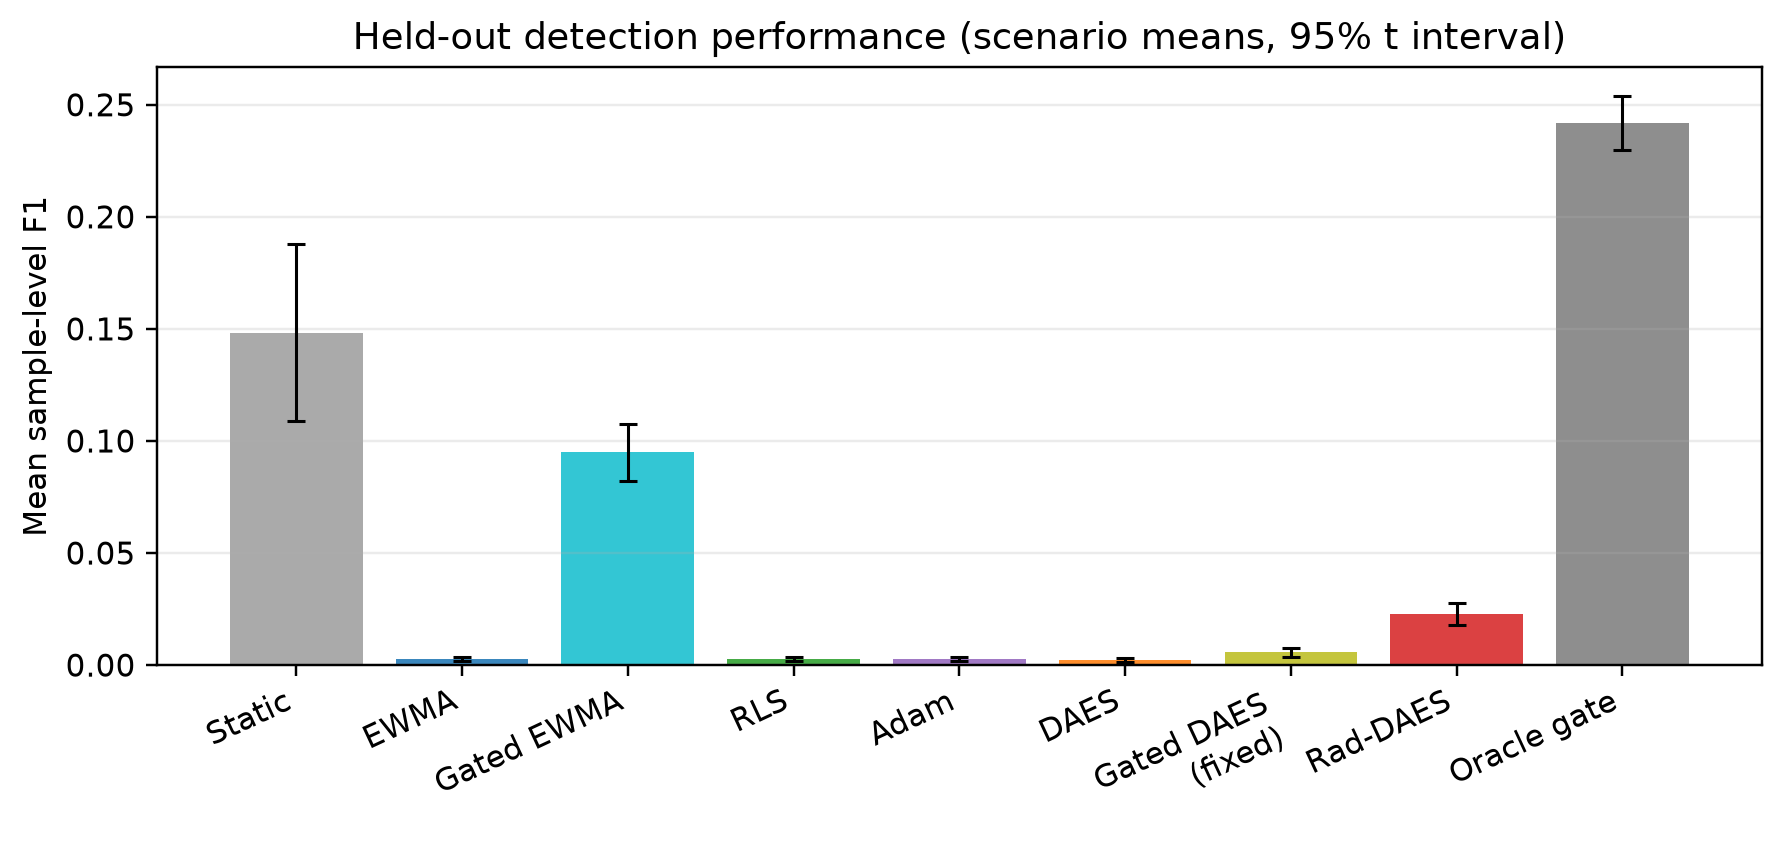
\includegraphics[width=0.92\linewidth]{../results/figures/fig_primary_f1.png}
\caption{Mean sample-level F1 by method. Error bars are 95\% Student-$t$ intervals across the 32 held-out scenario means. The oracle gate is a non-deployable reference.}
\label{fig:primary}
\end{figure}

\paragraph{The operating point dominates the ranking.}
The four methods whose development configurations satisfied the false-alarm constraint (EWMA, RLS, Adam, ungated DAES) have test F1 at most $0.003$ and detect at most 6\% of source events, with test FAR between 2.0 and 2.5/h. They are, in effect, blind at the calibrated operating point. The methods with visible detection either violate the false-alarm constraint or use labels: gated EWMA reaches F1 \GatedEWMAFone{} at \GatedEWMAFarPerHour{}/h, and Rad-DAES reaches \RadDAESFone{} at \RadDAESFarPerHour{}/h. \texttt{static} reaches \StaticFone{} only by alarming on 13.4\% of all samples. There is no deployable method in the matrix that is both sensitive and quiet. Figure~\ref{fig:tradeoff} plots this trade-off directly.

Table~\ref{tab:discrimination} separates threshold choice from separability. The oracle gate has the highest ROC AUC (0.773) and PR AUC (0.223), followed by \texttt{static} (0.728 and 0.128) and gated EWMA (0.691 and 0.089). Rad-DAES obtains ROC AUC \RadDAESRocAuc{} and PR AUC \RadDAESPrAuc{}, below both gated EWMA and \texttt{static}. The ordering is therefore not an artefact of one threshold: the DAES-based methods rank source samples less well than the simpler alternatives on these streams.

\begin{table}[t]
\centering
\caption{Threshold-free discrimination and gate behaviour. ROC/PR AUC use the pre-update score and do not depend on the alarm threshold. Event detection is the fraction of 960 source events with at least one alarm. Alarm fraction is the fraction of all evaluated samples that alarm. Release rate is the fraction of samples in which the sustained-exceedance release is active.}
\label{tab:discrimination}
\scriptsize
\setlength{\tabcolsep}{3pt}
\begin{tabular}{lccccccc}
\toprule
Method & ROC AUC & PR AUC & Event det. & Alarm frac. & Gate rej.\ clean & Gate rej.\ source & Release rate \\
\midrule
Static & 0.728 & 0.128 & 0.821 & 0.1341 & 0.397 & 0.630 & 0.0017 \\
EWMA & 0.622 & 0.031 & 0.060 & 0.0007 & 0.260 & 0.333 & 0.0000 \\
Gated EWMA & 0.691 & 0.089 & 0.406 & 0.0296 & 0.275 & 0.406 & 0.0000 \\
RLS & 0.622 & 0.031 & 0.060 & 0.0007 & 0.260 & 0.333 & 0.0000 \\
Adam & 0.637 & 0.033 & 0.056 & 0.0007 & 0.260 & 0.333 & 0.0000 \\
DAES & 0.600 & 0.024 & 0.054 & 0.0006 & 0.260 & 0.330 & 0.0000 \\
Gated DAES (fixed) & 0.558 & 0.019 & 0.059 & 0.0019 & 0.260 & 0.326 & 0.0000 \\
Rad-DAES & 0.629 & 0.036 & 0.105 & 0.0054 & 0.261 & 0.338 & 0.0000 \\
Oracle gate & 0.773 & 0.223 & 0.736 & 0.0039 & 0.260 & 0.485 & 0.0000 \\
\bottomrule
\end{tabular}

\end{table}

\begin{figure}[t]
\centering
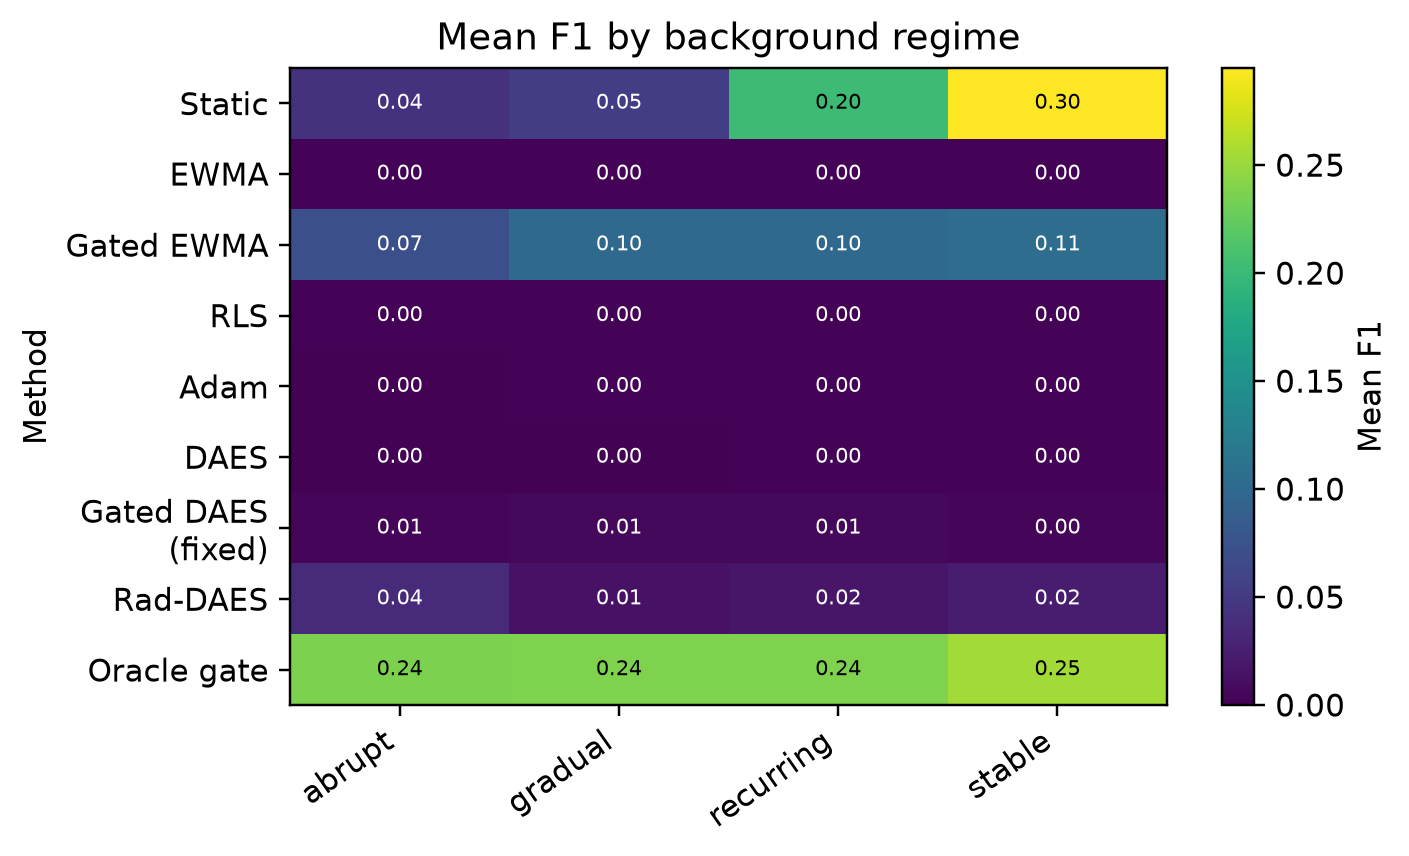
\includegraphics[width=0.92\linewidth]{../results/figures/fig_f1_by_regime.png}
\caption{Mean F1 by background regime. Each cell is the mean over the eight fault conditions and five seeds.}
\label{fig:regime}
\end{figure}

\begin{figure}[t]
\centering
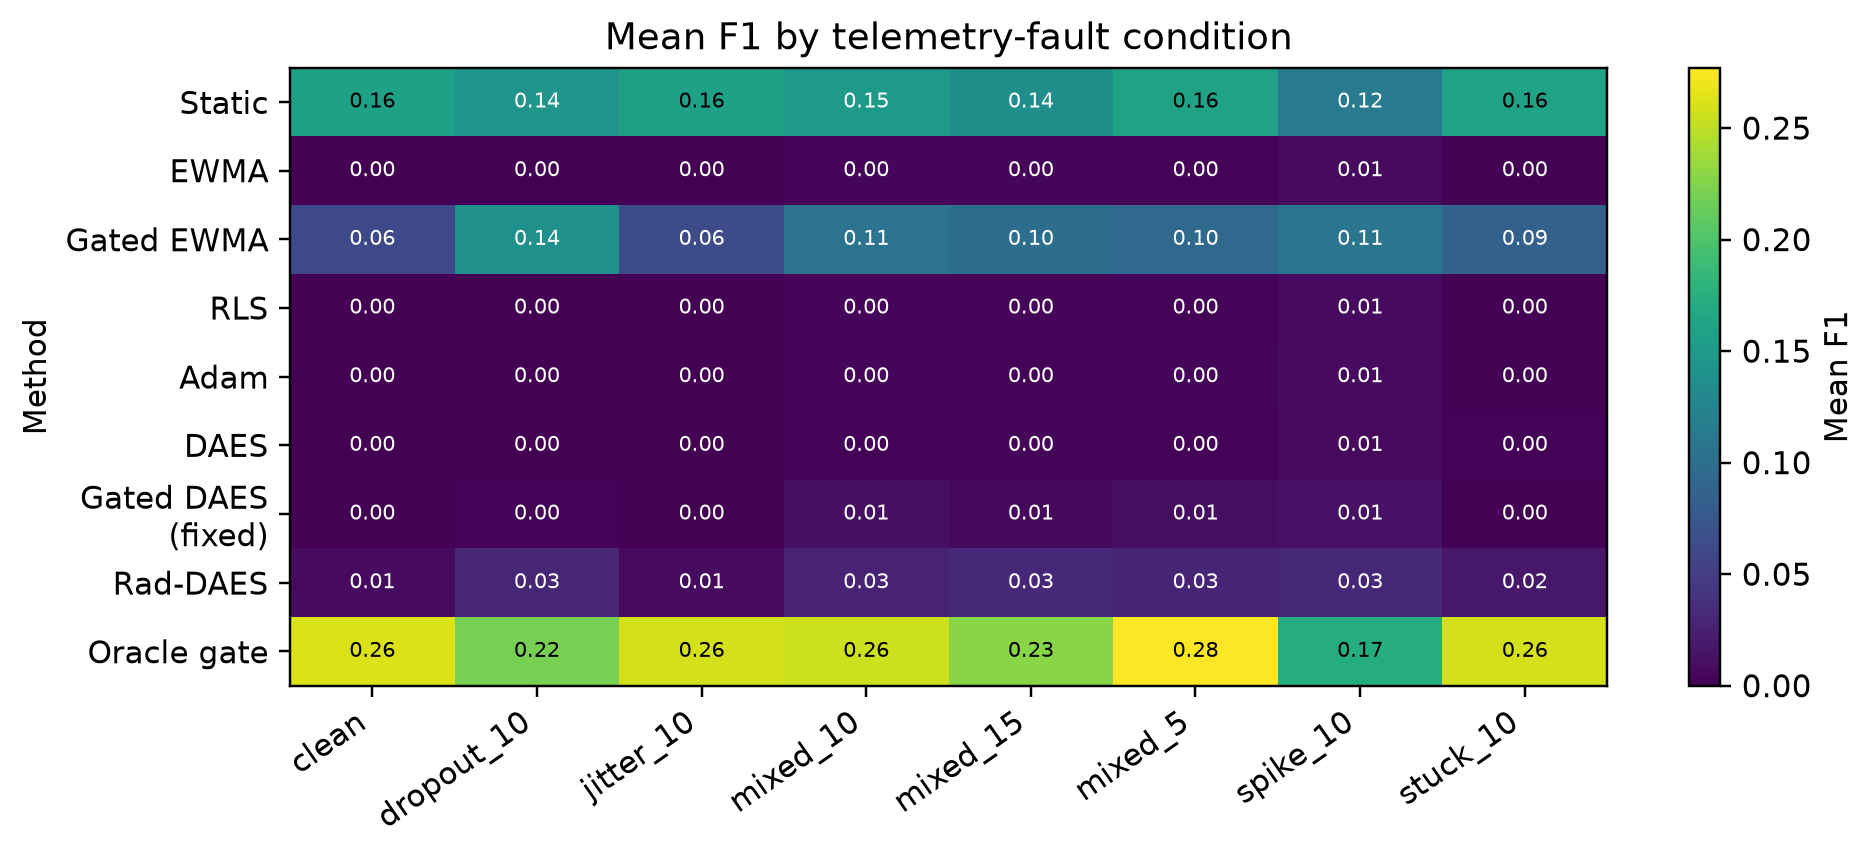
\includegraphics[width=0.98\linewidth]{../results/figures/fig_f1_by_fault.png}
\caption{Mean F1 by telemetry-fault condition. Each cell is the mean over the four regimes and five seeds.}
\label{fig:fault}
\end{figure}

\begin{figure}[t]
\centering
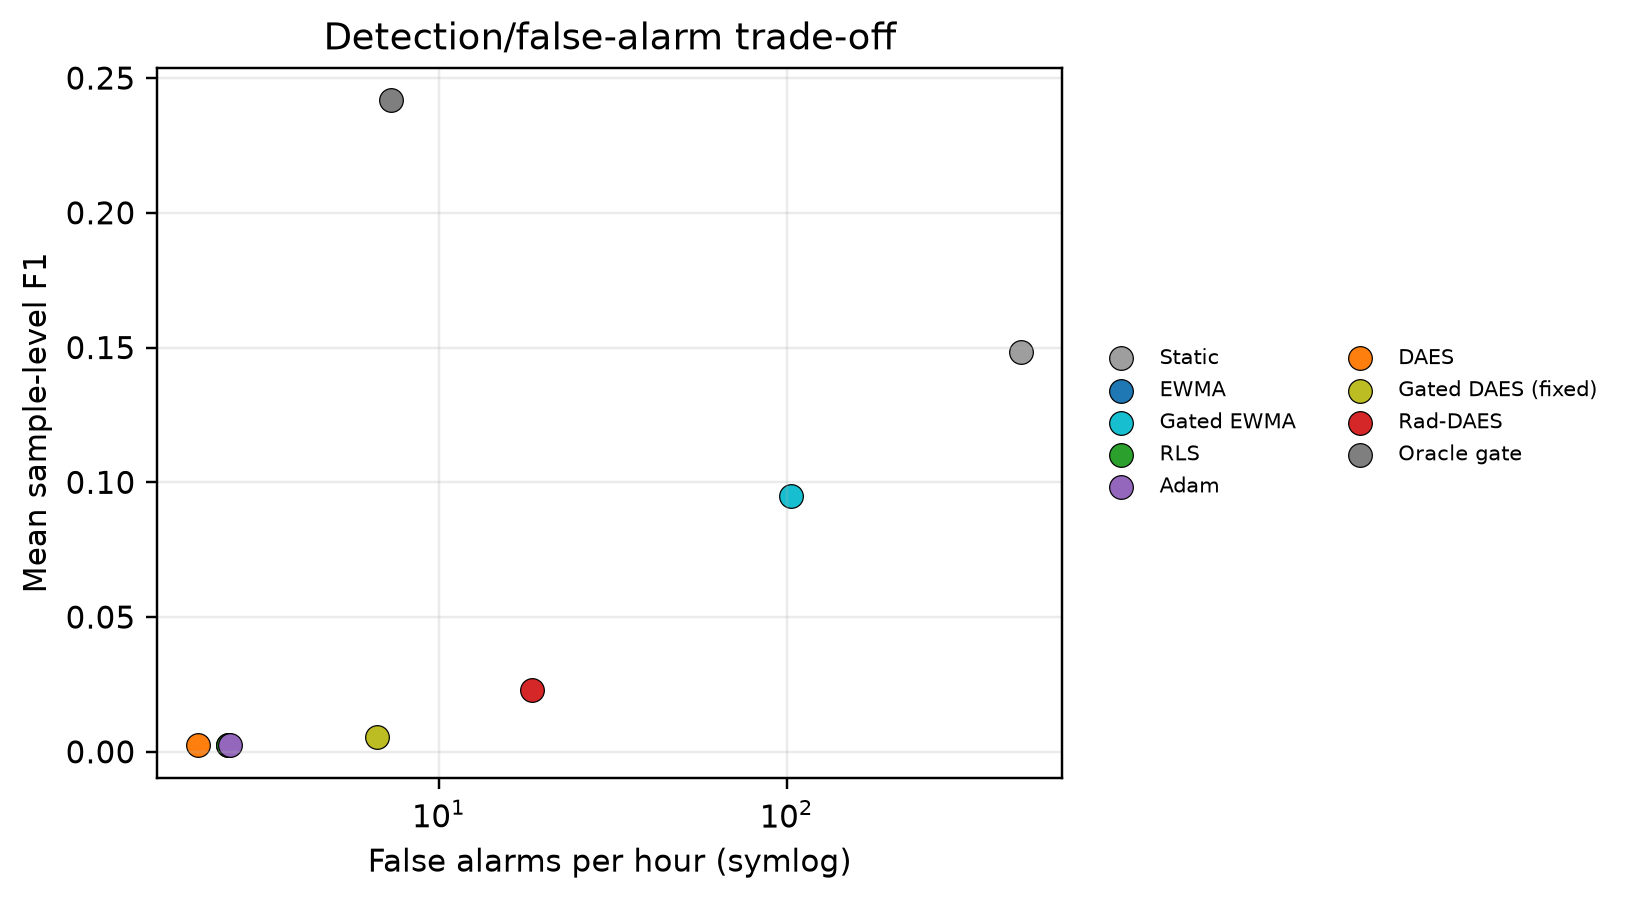
\includegraphics[width=0.78\linewidth]{../results/figures/fig_far_vs_f1.png}
\caption{Detection/false-alarm trade-off. The horizontal axis is symlog because static and some gated configurations produce very large drift-induced false-alarm burdens.}
\label{fig:tradeoff}
\end{figure}

\paragraph{Regime and fault structure.}
Figures~\ref{fig:regime} and~\ref{fig:fault} show that performance is not uniform. The recurring regime is the only regime not used for tuning; it is therefore the clearest check of whether a configuration generalises to a different drift shape. It does not rescue the candidate: Rad-DAES remains below gated EWMA and far below the oracle. Fault conditions change which samples are eligible for updating, so a method that looks adequate on clean streams can lose when dropout, jitter, stuck, or spike faults are present. The spike condition is the worst for false alarms: Rad-DAES reaches \RadDAESFarPerHour{}/h on average but 68.8/h under \texttt{spike\_10}, because a spike both alarms and freezes the update.

\paragraph{Gate behaviour.}
The gate rejects 26.1\% of clean samples and 33.8\% of source samples for Rad-DAES, and the sustained release is active on about $3\times10^{-6}$ of samples. The release is not merely rare: in the representative trace (Figure~\ref{fig:trace}) the consecutive-exceedance counter reaches 89 samples and then resets, one sample short of the 90-sample patience, so the model stays frozen through the step. The tracked mean remains near its pre-step value for roughly 350\,s while the true background has already moved by about 170 counts/s. The gate's source-rejection rate is the expected cost of protecting the background, but here the same mechanism also protects the background from the drift it is supposed to follow. Figure~\ref{fig:gate} summarises the rejection rates by sample type.

\begin{figure}[t]
\centering
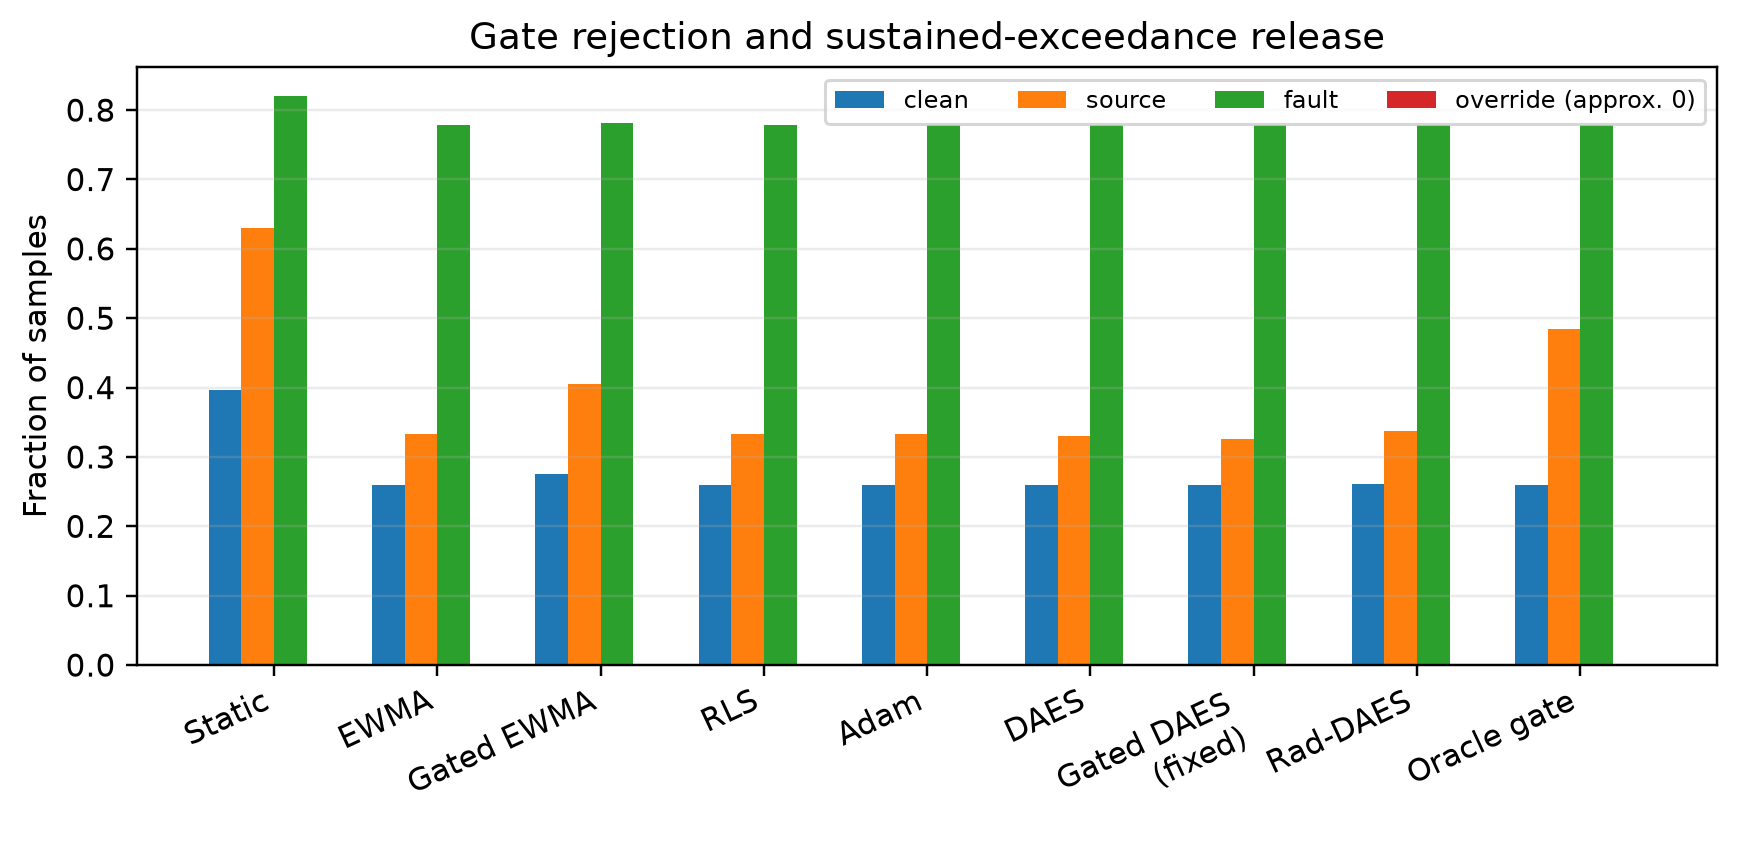
\includegraphics[width=0.92\linewidth]{../results/figures/fig_gate.png}
\caption{Gate rejection rates for clean, source, and fault samples, and the rate of sustained-exceedance release. A high source-rejection rate is the expected cost of protecting the background; it is also a recall risk.}
\label{fig:gate}
\end{figure}

\begin{figure}[t]
\centering
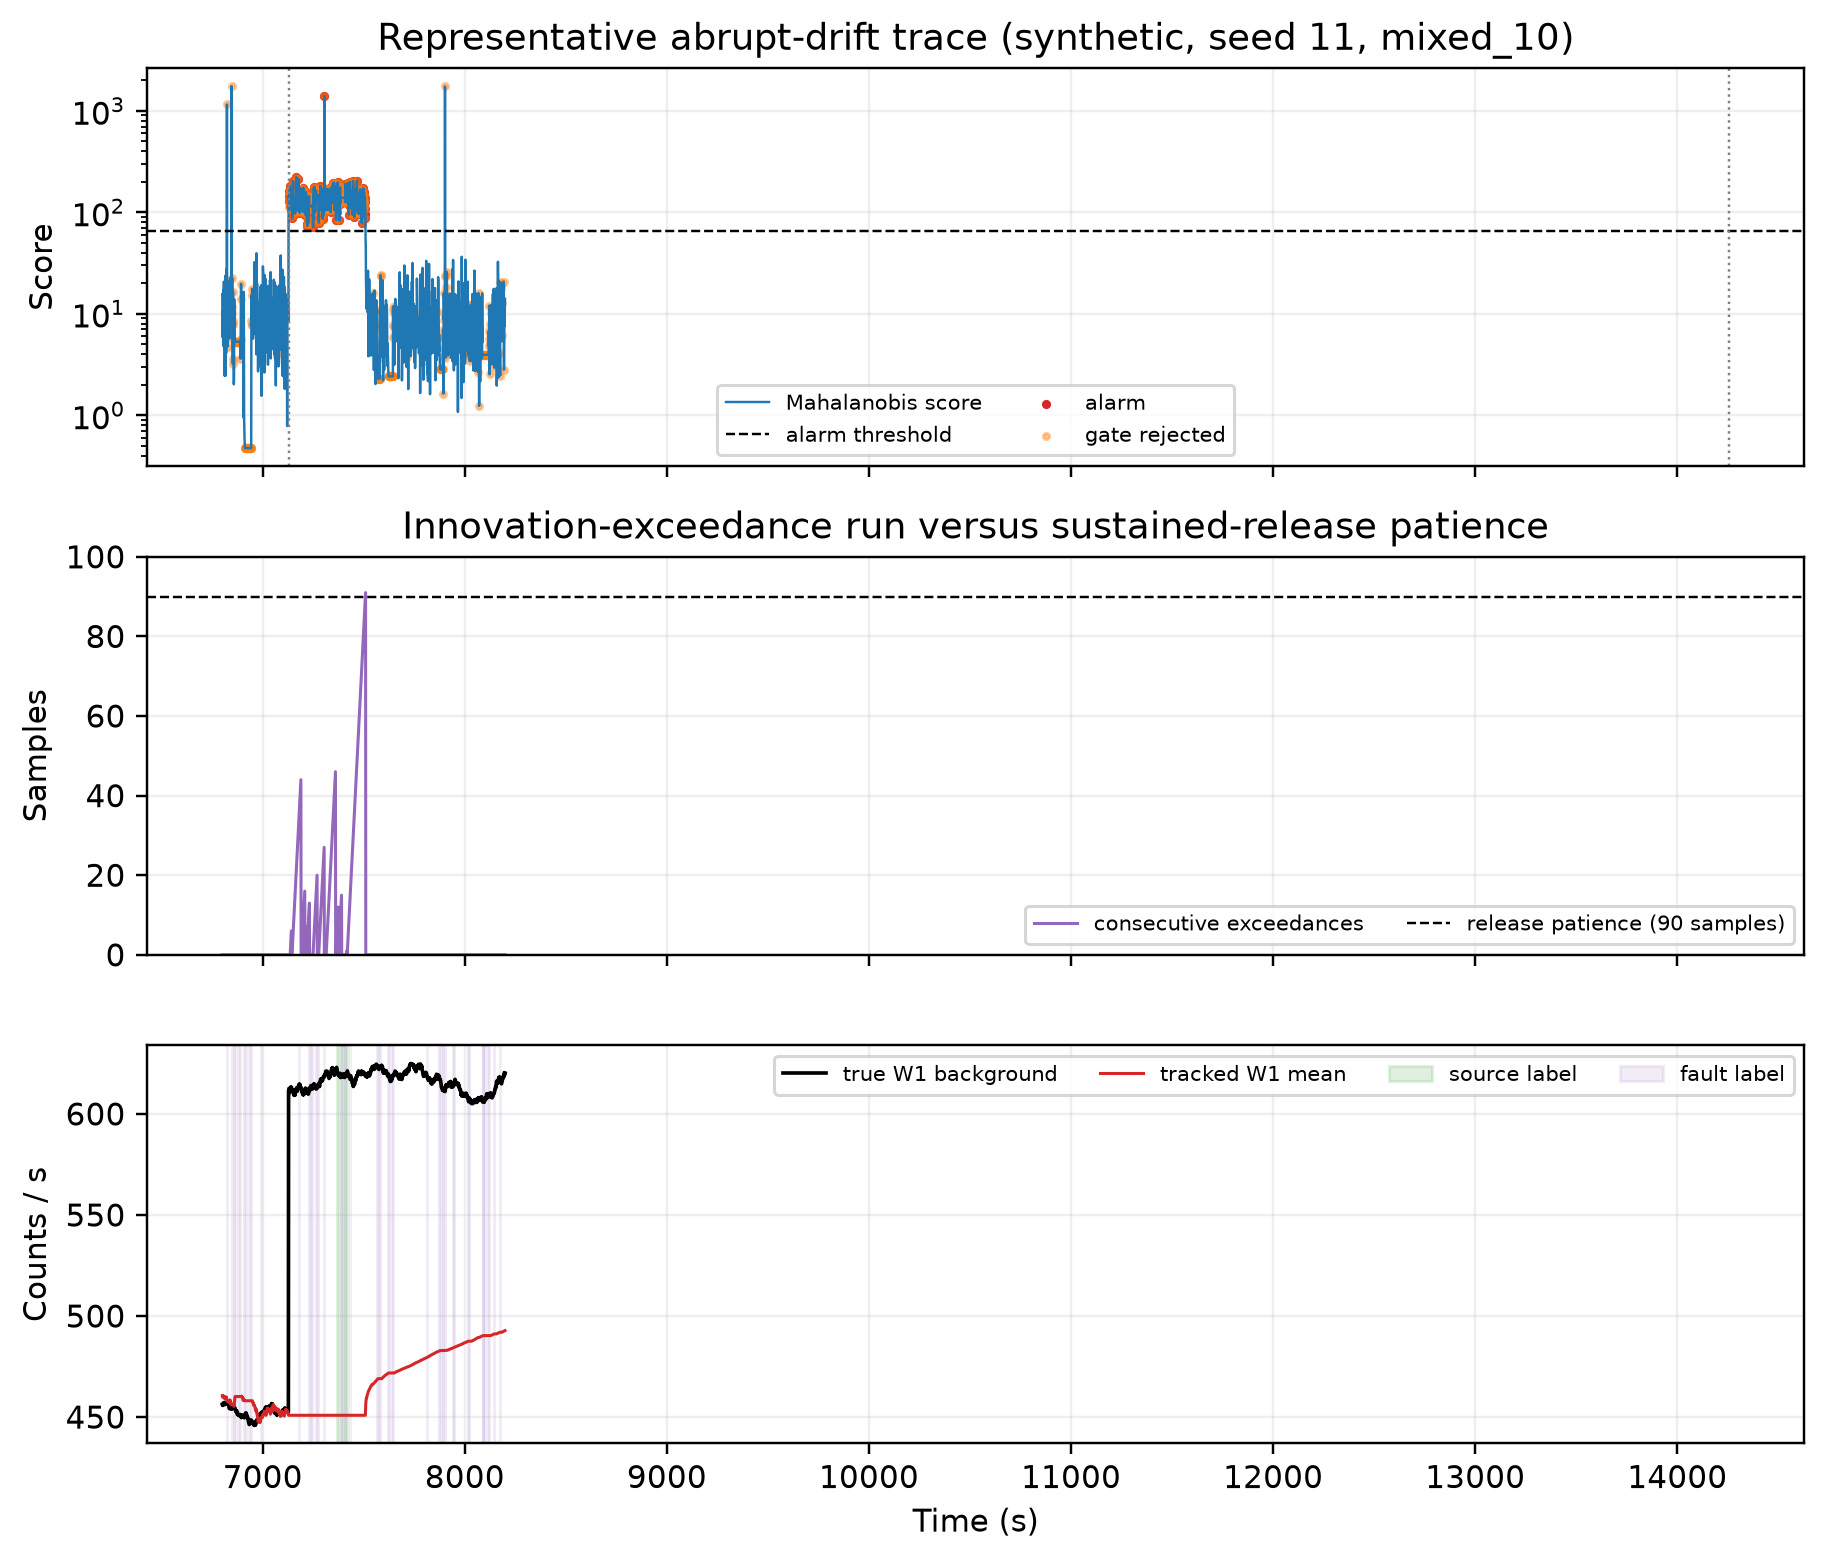
\includegraphics[width=0.95\linewidth]{../results/figures/fig_trace.png}
\caption{Representative abrupt-drift trace for Rad-DAES (synthetic, seed 11, \texttt{mixed\_10}). Top: pre-update score, alarms, and gate rejections. Middle: consecutive innovation exceedances versus the 90-sample release patience; the counter peaks at 89 and resets. Bottom: true and tracked W1 background, with source and fault labels.}
\label{fig:trace}
\end{figure}

\paragraph{Recovery and stability.}
Figure~\ref{fig:recovery} reports recovery time after abrupt steps. Recovery is defined as the first sample at which every window's relative mean error stays below 5\% for 30 consecutive samples; an event that never meets the condition is not silently counted as a success. Rad-DAES recovers 55 of 80 abrupt-step events with a mean recovery time of \RadDAESRecoveryMean{}\,s; gated EWMA recovers all 80 at \GatedEWMARecoveryMean{}\,s but with a much higher false-alarm burden; ungated EWMA and RLS recover all 80 at about 399\,s while remaining nearly blind to sources; \texttt{static} recovers none. Recovery and detection therefore pull in opposite directions in this matrix, and no method achieves both.

\begin{figure}[t]
\centering
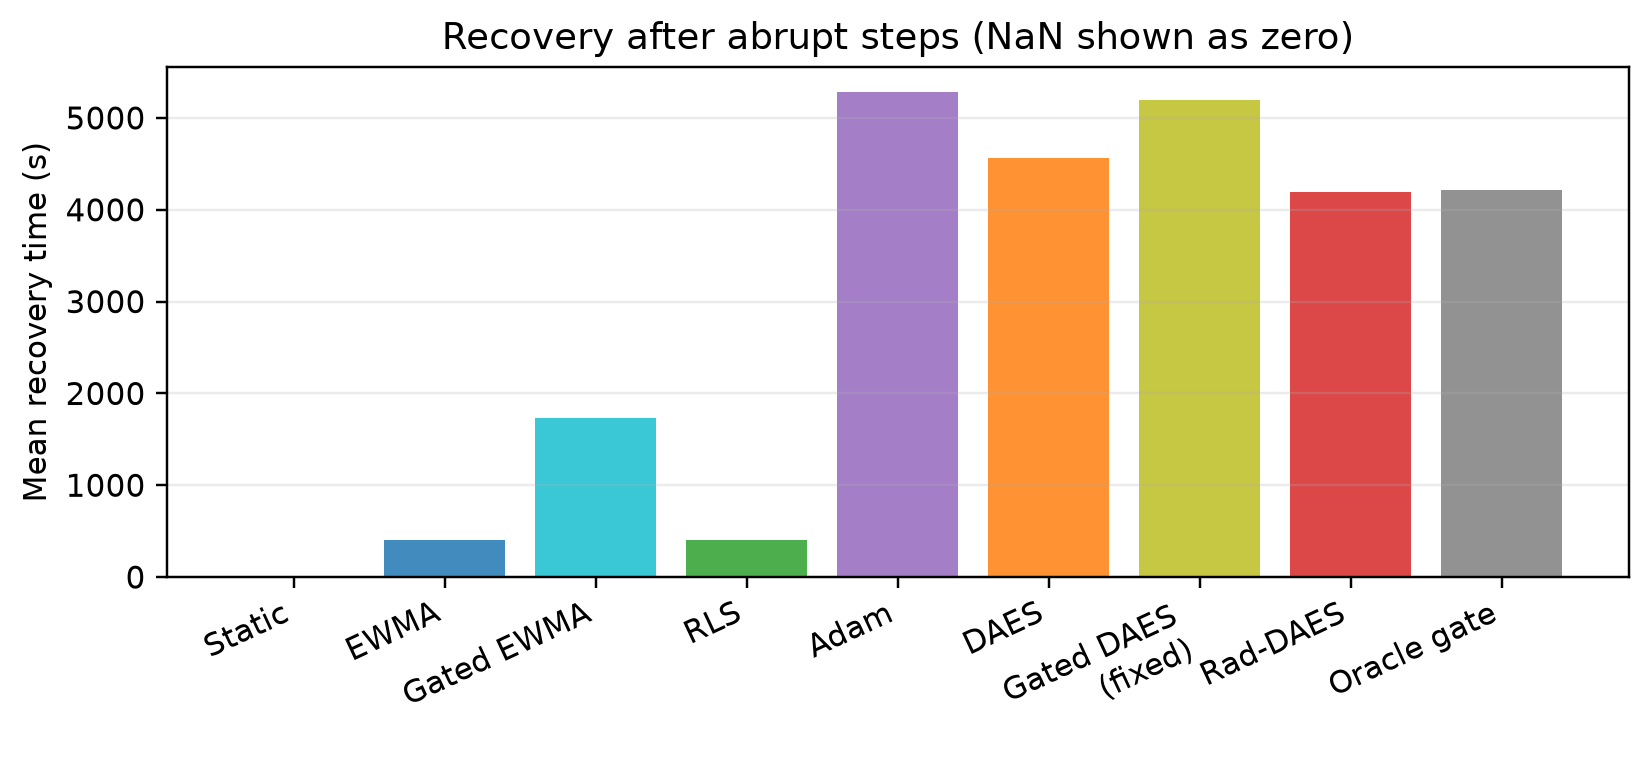
\includegraphics[width=0.78\linewidth]{../results/figures/fig_recovery.png}
\caption{Mean recovery time after abrupt steps. Missing values are shown as zero only for display; they are not treated as recovered in the tables.}
\label{fig:recovery}
\end{figure}

\begin{table}[t]
\centering
\caption{Paired differences (Rad-DAES minus the named method) over matched scenario/seed pairs. Each pair is one held-out run; the 160 pairs are 32 scenarios $\times$ 5 seeds, and the five seeds of a scenario are treated as independent observations, so within-scenario clustering is not modelled. Positive F1 is better; positive FAR and BG are worse. Intervals are descriptive 95\% Student-$t$ intervals and are not multiplicity-corrected.}
\label{tab:paired}
\scriptsize
\begin{tabular}{llccc}
\toprule
Comparison & Metric & Mean difference & 95\% CI & Pairs \\
\midrule
Rad-DAES minus Static & f1 & -0.125 & [-0.146, -0.105] & 160 \\
Rad-DAES minus Static & far\_per\_hour & -453.9 & [-534.8, -372.9] & 160 \\
Rad-DAES minus Static & bg\_rel\_error & -0.029 & [-0.034, -0.024] & 160 \\
Rad-DAES minus EWMA & f1 & 0.020 & [0.013, 0.027] & 160 \\
Rad-DAES minus EWMA & far\_per\_hour & 16.032 & [6.324, 25.741] & 160 \\
Rad-DAES minus EWMA & bg\_rel\_error & 0.010 & [0.008, 0.012] & 160 \\
Rad-DAES minus Gated EWMA & f1 & -0.072 & [-0.081, -0.063] & 160 \\
Rad-DAES minus Gated EWMA & far\_per\_hour & -84.240 & [-122.8, -45.653] & 160 \\
Rad-DAES minus Gated EWMA & bg\_rel\_error & 0.008 & [0.006, 0.010] & 160 \\
Rad-DAES minus RLS & f1 & 0.020 & [0.013, 0.027] & 160 \\
Rad-DAES minus RLS & far\_per\_hour & 16.032 & [6.324, 25.741] & 160 \\
Rad-DAES minus RLS & bg\_rel\_error & 0.010 & [0.008, 0.012] & 160 \\
Rad-DAES minus Adam & f1 & 0.020 & [0.014, 0.027] & 160 \\
Rad-DAES minus Adam & far\_per\_hour & 16.008 & [6.291, 25.726] & 160 \\
Rad-DAES minus Adam & bg\_rel\_error & -0.002 & [-0.004, -0.000] & 160 \\
Rad-DAES minus DAES & f1 & 0.020 & [0.014, 0.027] & 160 \\
Rad-DAES minus DAES & far\_per\_hour & 16.478 & [6.720, 26.236] & 160 \\
Rad-DAES minus DAES & bg\_rel\_error & -0.012 & [-0.017, -0.007] & 160 \\
Rad-DAES minus Gated DAES (fixed) & f1 & 0.017 & [0.011, 0.023] & 160 \\
Rad-DAES minus Gated DAES (fixed) & far\_per\_hour & 11.860 & [2.278, 21.441] & 160 \\
Rad-DAES minus Gated DAES (fixed) & bg\_rel\_error & -0.043 & [-0.044, -0.043] & 160 \\
Rad-DAES minus Oracle gate & f1 & -0.219 & [-0.231, -0.207] & 160 \\
Rad-DAES minus Oracle gate & far\_per\_hour & 11.217 & [1.634, 20.799] & 160 \\
Rad-DAES minus Oracle gate & bg\_rel\_error & 0.011 & [0.010, 0.012] & 160 \\
\bottomrule
\end{tabular}

\end{table}

\paragraph{Tuning and fallbacks.}
Table~\ref{tab:tuning} records the selected development configuration for each method. Four of the nine methods used a fallback, meaning that no candidate met both the background-error and false-alarm constraints on the development scenarios. Rad-DAES selected the largest gain in the grid ($\gamma=0.5$) with a development FAR of 28.6/h, more than fourteen times the constraint; gated EWMA selected the smallest EWMA weight but still had a development FAR of 99.4/h. The oracle gate selected the smallest gain ($\gamma=0.05$) and had a development FAR of 12.5/h. The oracle's advantage is therefore not an isolated gate effect: it combines perfect labelling with a ten-fold gentler step, and the two cannot be separated in this matrix. The selected configurations were frozen before the test matrix.

\begin{table}[t]
\centering
\caption{Selected development configurations and development means. ``Fallback'' means no candidate satisfied both the background-error and false-alarm constraints.}
\label{tab:tuning}
\scriptsize
\begin{tabular}{llcccc}
\toprule
Method & Selected configuration & Status & Dev F1 & Dev BG & Dev FAR/h \\
\midrule
Static & \texttt{default} & fixed & 0.137 & 0.0644 & 647.7 \\
EWMA & \texttt{ewma\_alpha=0.02} & feasible & 0.004 & 0.0136 & 1.11 \\
Gated EWMA & \texttt{ewma\_alpha=0.005;gate\_quantile=0.999} & fallback & 0.078 & 0.0148 & 99.36 \\
RLS & \texttt{rls\_forgetting=0.98} & feasible & 0.004 & 0.0136 & 1.11 \\
Adam & \texttt{adam\_learning\_rate=0.02} & feasible & 0.005 & 0.0261 & 1.09 \\
DAES & \texttt{daes\_gain=0.2} & feasible & 0.004 & 0.0417 & 1.05 \\
Gated DAES (fixed) & \texttt{daes\_gain=0.5;gate\_quantile=0.995} & fallback & 0.011 & 0.0692 & 12.42 \\
Rad-DAES & \texttt{daes\_gain=0.5;gate\_quantile=0.999} & fallback & 0.036 & 0.0257 & 28.64 \\
Oracle gate & \texttt{daes\_gain=0.05} & fallback & 0.228 & 0.0147 & 12.48 \\
\bottomrule
\end{tabular}

\end{table}

\section{Discussion}

The experiment was designed to test a trade-off, not to demonstrate that a new method wins. The answer is negative, and three mechanisms explain most of it.

\emph{First, the innovation guard confuses drift with a source.} A persistent background step produces a sustained score above the gate threshold, so the gate freezes the mean precisely when the mean needs to move. The 90-sample release was intended to break this deadlock, but it requires an uninterrupted run of exceedances; Poisson noise and the oscillating score reset the counter. In the representative trace the counter peaks at 89 and resets. The result is a frozen model, a long alarm burst, and a slow recovery. This is a design failure of the release rule, not a tuning issue: the rule is brittle by construction because it depends on a run length in a noisy sequence.

\emph{Second, the adaptive background appears to absorb source energy.} Both the mean and the covariance update on a 50-sample time constant, comparable to the 20--60\,s source duration. During the ramp of a source event the score is still below the gate threshold, so the gate passes those samples; the mean then moves toward the source and the covariance learns its outer product, and the score for the peak falls. This is consistent with the threshold-free results: \texttt{static}, which updates neither the mean nor the covariance, has ROC AUC 0.728, while the adaptive methods have ROC AUC between 0.558 and 0.691. We did not run a covariance-frozen or mean-frozen ablation, so the two channels are not separated experimentally; the static-versus-adaptive contrast supports the general mechanism, not the share attributable to covariance. It is the most plausible explanation for why the ungated methods detect only about 6\% of events despite a nominal 3--8$\sigma$ source amplitude.

\emph{Third, the selection rule was infeasible.} The development constraint (FAR $\le 2$/h, background error $\le 0.10$) could not be met by any gated configuration under abrupt drift. The fallback rule then chose configurations that violated the FAR constraint by one to two orders of magnitude, and those configurations were frozen for test. The four feasible methods were feasible only because they were nearly blind. The protocol therefore did not compare methods at a common, achievable operating point; it compared blind methods against noisy ones. A matched-FAR evaluation, or a prespecified ROC/PR analysis, would have been more informative. The ROC/PR table is reported here as a secondary analysis, but it was not the basis of the selection rule.

The practical implication is that the three decisions should not share one score. A drift detector, a source detector, and a telemetry-integrity check answer different questions \citep{gama2014survey,isermann2005model}; using the same Mahalanobis score for gating and alarming creates the coupling observed here. A two-timescale covariance (fast for the mean, slow or robust for the detector), or a covariance that is frozen during suspected sources, is a concrete next step. None of these is implemented or validated in this draft.

The draft does not establish that Rad-DAES is novel. The literature review here is structured but not a full systematic review; the closest related work on portal data and concept drift is cited only to frame the problem. A novelty claim would require a protocol-driven review and a direct comparison on public data.

\section{Limitations and threats to validity}

\begin{itemize}
  \item \textbf{No real data.} RADAI requires an account and a large download; PyRIID requires a compatible Python environment and spectra conversion; the JRC reference spectra are not a continuous portal stream. No credentials were used and no real stream was parsed. Gate~1 of the project plan is a partial failure.
  \item \textbf{Synthetic generator.} The regimes, source templates, amplitudes, and fault rates are design choices. They are not fitted to measured background. The Poisson model ignores detector resolution, dead time, and spectrum unfolding \citep{knoll2010radiation}. The $\sin^2$ source profile makes the peak narrow, which penalises sample-level F1; event-level detection is reported to reduce that sensitivity, but it does not eliminate it. The design is reported in the form recommended for simulation studies \citep{morris2019simulation}, but a synthetic study cannot substitute for measured streams.
  \item \textbf{Mechanism inferred, not isolated.} The adaptive-background explanation (mean and covariance) is supported by the static-versus-adaptive contrast and by the saved traces, but no covariance-frozen or mean-frozen ablation was run, so the two channels are not separated. The gate-deadlock explanation is directly visible in one representative trace; the 89-versus-90 near miss is illustrative, not a distributional estimate.
  \item \textbf{Small seed budget.} Five seeds were evaluated per scenario. The primary 95\% confidence intervals are calculated across the 32 scenario means after averaging the five seeds within each scenario. These intervals are descriptive and conditional on the fixed scenario design. They do not quantify uncertainty beyond the selected scenarios or account for model misspecification \citep{greenland2016statistical}.
  \item \textbf{No multiplicity correction.} The scenario-level and paired comparisons are descriptive. A claim of statistical significance is not made, and no false-discovery-rate procedure is applied \citep{benjamini1995controlling}.
  \item \textbf{Design choices.} The 90-sample (90\,s) release, the 0.5--1.5\,s timing bound, the 0.25--3.5 Fano bounds, the 0.25 covariance floor, the 50-sample covariance time constant, and the six windows are choices, not validated constants. Sensitivity analyses are future work.
  \item \textbf{Threshold transfer.} Thresholds calibrated on clean stable streams do not transfer to drift regimes: even the oracle gate has 7.3 false alarms/h on test. The 1/h calibration target is therefore not an operational guarantee, and portal false-alarm testing requires a broader operating-characteristic study than the one reported here \citep{burr2007alarm,leber2020false}.
  \item \textbf{DAES provenance.} The DAES equations follow the supplied scalar reference implementation. The matrix update in some generated planning material is not implemented as DAES. The wrapper's use of a Gaussian quasi-likelihood Hessian is an adaptation, not a theorem.
  \item \textbf{No field readiness.} Runtime is offline Python on synthetic arrays. No hardware latency, network delay, calibration uncertainty, or regulatory requirement is modelled.
\end{itemize}

\section{Reproducibility}

{\sloppy
The repository is self-contained and separate from the unrelated projects that share the workspace. The synthetic generator, gate, DAES controller, background model, detector, runner, tests, scripts, raw CSV files, tables, and figures are included. The packaging follows the reproducibility principle that data, code, and the computational narrative should be inspectable together \citep{peng2011reproducible}. The main commands are:\par}
\begin{verbatim}
python -m pip install -e .
python -m pytest -q
python scripts/run_benchmarks.py --mode full --output results/raw
python scripts/aggregate_results.py
python scripts/make_figures.py
python scripts/audit_results.py
\end{verbatim}
The runner writes a manifest with Python and package versions, configuration hashes, seed lists, and run counts. Every table and figure is generated from saved CSV or trace files; no result is typed into the manuscript by hand. The audit script checks matrix completeness, the frozen selection and thresholds, a determinism spot-check of saved rows, config hashes, and the presence of every table, figure, and macro used here. The original DAES reference file was read from an external snapshot for interface documentation and was not vendored or modified. Its SHA-256 and the archive SHA-256 are recorded in \texttt{docs/daes\_interface.md}.

{\sloppy
The raw run was launched with \texttt{--output results} and then moved into \texttt{results/raw/} to match the layout read by the aggregation and audit scripts; the only edited field was the trace-path column of \texttt{trace\_index.csv}. This is documented in \texttt{results/raw/README.md}.\par}

\section{Conclusion}

This draft delivers a small, complete, reproducible synthetic study of guarded drift-aware background tracking, and its result is negative. Rad-DAES does not improve the detection/false-alarm trade-off on these streams: its F1 is \RadDAESFone{} at \RadDAESFarPerHour{}/h, while the four false-alarm-compliant methods are nearly blind and the non-deployable oracle reaches only \BestValue{}. The traces identify two concrete failure modes, gate-induced freezing under drift and apparent adaptive-background contamination during source ramps, and the development selection rule is shown to be infeasible at the prespecified operating point. The value of the draft is the auditable pipeline and the explicit evidence boundary, not a claim that the candidate method is ready for a portal.

\bibliographystyle{plainnat}
\bibliography{references}

\appendix
\section{Implementation map}

\begin{table}[htbp]
\centering
\caption{Where each component is implemented and tested. Package paths are relative to \texttt{src/rad\_daes/}; script, test, and report paths are relative to the repository root.}
\small
\setlength{\tabcolsep}{4pt}
\begin{tabular}{lll}
\toprule
Component & Source & Test \\
\midrule
Synthetic streams & \texttt{data/synthetic.py} & \texttt{tests/test\_synthetic.py} \\
Window definitions & \texttt{preprocessing/windows.py} & configuration checks \\
Background model & \texttt{background/model.py} & \texttt{tests/test\_background.py} \\
Telemetry gate & \texttt{telemetry/gate.py} & \texttt{tests/test\_gate.py} \\
DAES controller & \texttt{adaptation/daes.py} & \texttt{tests/test\_daes.py} \\
Detector & \texttt{detection/detector.py} & runner integration \\
Metrics & \texttt{evaluation/metrics.py} & \texttt{tests/test\_metrics.py} \\
Runner and calibration & \texttt{evaluation/runner.py} & \texttt{tests/test\_runner.py} \\
Aggregation & \texttt{scripts/aggregate\_results.py} & table checks \\
Audit & \texttt{scripts/audit\_results.py} & \texttt{results/audit\_report.md} \\
\bottomrule
\end{tabular}
\end{table}

\section{Protocol revisions}

The source-placement bug, the sustained-exceedance release, the covariance floor, and the midpoint source profile were fixed on 28 October 2026 before the held-out matrix was run. The revision log is in \texttt{docs/protocol.md}. No held-out result was inspected before these changes. After the frozen test matrix was complete, the threshold-free ROC/PR table and the event-level detection summary were added as secondary analyses; they are computed from columns already saved by the frozen run, and the primary estimand and selection rule were not changed.

\clearpage
\section{Artifact inventory}

Table~\ref{tab:artifacts} lists the paths a reader needs in order to inspect or rerun the study. Counts describe the working repository of 28 October 2026 and exclude Python caches and \LaTeX{} build byproducts; the submission mirror differs only in that the cover-letter DOCX sits at the bundle root, so its \texttt{paper/} directory has six files.

\begin{table}[htbp]
\centering
\caption{Frozen artifact inventory. File counts exclude \texttt{\_\_pycache\_\_} directories.}
\label{tab:artifacts}
\small
\setlength{\tabcolsep}{4pt}
\begin{tabular}{llr}
\toprule
Path & Contents & Files \\
\midrule
\texttt{src/rad\_daes/} & Generator, gate, DAES controller, model, detector, metrics, runner & 16 \\
\texttt{configs/} & Data, model, and experiment configuration & 3 \\
\texttt{tests/} & Unit and integration tests (44 passing) & 7 \\
\texttt{results/raw/} & Calibration, development, and test CSVs; manifest; 4 traces & 13 \\
\texttt{results/tables/} & CSV, \LaTeX{} tables, and generated macros & 16 \\
\texttt{results/figures/} & Seven PNG figures & 7 \\
\texttt{docs/} & Protocol, decisions, DAES interface, results summary, checklist & 8 \\
\texttt{paper/} & Manuscript source, PDF, cover letter, bibliography, supplementary note & 7 \\
\bottomrule
\end{tabular}
\end{table}

The primary test artifact is \texttt{results/raw/test\_runs.csv} (1{,}440 rows). The audit report is regenerated by \texttt{scripts/audit\_results.py} and records 22 checks. No real radiation data are included, because none were obtained (Section~6).

\end{document}
"
\providecommand{\PaperSize}{letterpaper}
\usepackage[\PaperSize,margin=1in]{geometry}
\usepackage{amsmath,amssymb}
\usepackage{booktabs}
\usepackage{graphicx}
\usepackage{siunitx}
\usepackage[hidelinks]{hyperref}
\usepackage[numbers,sort]{natbib}
\usepackage{xcolor}
\usepackage{caption}
\usepackage{subcaption}

\hypersetup{
  pdftitle={Guarded Drift-Aware Background Tracking for Synthetic Radiation-Portal Count Streams: A Reproducible Benchmark and a Negative Result},
  pdfauthor={Tripti Kumari, Chayan Ojha, Mriganko Dey, Ankita Polley},
  pdfsubject={B.Tech group project, Department of Computer Science and Engineering (AI \& ML), Narula Institute of Technology, Agarpara}
}

% Generated by scripts/aggregate_results.py. Do not edit by hand.
\newcommand{\StaticFone}{0.148}
\newcommand{\StaticFarPerHour}{472.4}
\newcommand{\StaticBgRelError}{0.055}
\newcommand{\StaticRecall}{0.370}
\newcommand{\StaticPrecision}{0.249}
\newcommand{\StaticRecoveryMean}{---}
\newcommand{\EWMAFone}{0.003}
\newcommand{\EWMAFarPerHour}{2.476}
\newcommand{\EWMABgRelError}{0.015}
\newcommand{\EWMARecall}{0.002}
\newcommand{\EWMAPrecision}{0.089}
\newcommand{\EWMARecoveryMean}{399.1}
\newcommand{\GatedEWMAFone}{0.095}
\newcommand{\GatedEWMAFarPerHour}{102.7}
\newcommand{\GatedEWMABgRelError}{0.017}
\newcommand{\GatedEWMARecall}{0.121}
\newcommand{\GatedEWMAPrecision}{0.473}
\newcommand{\GatedEWMARecoveryMean}{1734}
\newcommand{\RLSFone}{0.003}
\newcommand{\RLSFarPerHour}{2.476}
\newcommand{\RLSBgRelError}{0.015}
\newcommand{\RLSRecall}{0.002}
\newcommand{\RLSPrecision}{0.089}
\newcommand{\RLSRecoveryMean}{399.1}
\newcommand{\AdamFone}{0.003}
\newcommand{\AdamFarPerHour}{2.500}
\newcommand{\AdamBgRelError}{0.028}
\newcommand{\AdamRecall}{0.002}
\newcommand{\AdamPrecision}{0.078}
\newcommand{\AdamRecoveryMean}{5286}
\newcommand{\DAESFone}{0.002}
\newcommand{\DAESFarPerHour}{2.031}
\newcommand{\DAESBgRelError}{0.038}
\newcommand{\DAESRecall}{0.001}
\newcommand{\DAESPrecision}{0.054}
\newcommand{\DAESRecoveryMean}{4564}
\newcommand{\GatedDAESFixedFone}{0.006}
\newcommand{\GatedDAESFixedFarPerHour}{6.649}
\newcommand{\GatedDAESFixedBgRelError}{0.069}
\newcommand{\GatedDAESFixedRecall}{0.004}
\newcommand{\GatedDAESFixedPrecision}{0.054}
\newcommand{\GatedDAESFixedRecoveryMean}{5196}
\newcommand{\RadDAESFone}{0.023}
\newcommand{\RadDAESFarPerHour}{18.508}
\newcommand{\RadDAESBgRelError}{0.025}
\newcommand{\RadDAESRecall}{0.024}
\newcommand{\RadDAESPrecision}{0.142}
\newcommand{\RadDAESRecoveryMean}{4198}
\newcommand{\OracleGateFone}{0.242}
\newcommand{\OracleGateFarPerHour}{7.292}
\newcommand{\OracleGateBgRelError}{0.014}
\newcommand{\OracleGateRecall}{0.158}
\newcommand{\OracleGatePrecision}{0.721}
\newcommand{\OracleGateRecoveryMean}{4213}
\newcommand{\BestMethod}{Oracle gate}
\newcommand{\BestValue}{0.242}
\newcommand{\NScenarios}{32}
\newcommand{\StaticRocAuc}{0.728}
\newcommand{\StaticPrAuc}{0.128}
\newcommand{\StaticEventDetection}{0.821}
\newcommand{\StaticAlarmFraction}{0.134}
\newcommand{\StaticGateRejectClean}{0.397}
\newcommand{\StaticGateRejectSource}{0.630}
\newcommand{\StaticGateOverrideRate}{0.002}
\newcommand{\EWMARocAuc}{0.622}
\newcommand{\EWMAPrAuc}{0.031}
\newcommand{\EWMAEventDetection}{0.060}
\newcommand{\EWMAAlarmFraction}{0.001}
\newcommand{\EWMAGateRejectClean}{0.260}
\newcommand{\EWMAGateRejectSource}{0.333}
\newcommand{\EWMAGateOverrideRate}{0.000}
\newcommand{\GatedEWMARocAuc}{0.691}
\newcommand{\GatedEWMAPrAuc}{0.089}
\newcommand{\GatedEWMAEventDetection}{0.406}
\newcommand{\GatedEWMAAlarmFraction}{0.030}
\newcommand{\GatedEWMAGateRejectClean}{0.275}
\newcommand{\GatedEWMAGateRejectSource}{0.406}
\newcommand{\GatedEWMAGateOverrideRate}{0.000}
\newcommand{\RLSRocAuc}{0.622}
\newcommand{\RLSPrAuc}{0.031}
\newcommand{\RLSEventDetection}{0.060}
\newcommand{\RLSAlarmFraction}{0.001}
\newcommand{\RLSGateRejectClean}{0.260}
\newcommand{\RLSGateRejectSource}{0.333}
\newcommand{\RLSGateOverrideRate}{0.000}
\newcommand{\AdamRocAuc}{0.637}
\newcommand{\AdamPrAuc}{0.033}
\newcommand{\AdamEventDetection}{0.056}
\newcommand{\AdamAlarmFraction}{0.001}
\newcommand{\AdamGateRejectClean}{0.260}
\newcommand{\AdamGateRejectSource}{0.333}
\newcommand{\AdamGateOverrideRate}{0.000}
\newcommand{\DAESRocAuc}{0.600}
\newcommand{\DAESPrAuc}{0.024}
\newcommand{\DAESEventDetection}{0.054}
\newcommand{\DAESAlarmFraction}{0.001}
\newcommand{\DAESGateRejectClean}{0.260}
\newcommand{\DAESGateRejectSource}{0.330}
\newcommand{\DAESGateOverrideRate}{0.000}
\newcommand{\GatedDAESFixedRocAuc}{0.558}
\newcommand{\GatedDAESFixedPrAuc}{0.019}
\newcommand{\GatedDAESFixedEventDetection}{0.059}
\newcommand{\GatedDAESFixedAlarmFraction}{0.002}
\newcommand{\GatedDAESFixedGateRejectClean}{0.260}
\newcommand{\GatedDAESFixedGateRejectSource}{0.326}
\newcommand{\GatedDAESFixedGateOverrideRate}{0.000}
\newcommand{\RadDAESRocAuc}{0.629}
\newcommand{\RadDAESPrAuc}{0.036}
\newcommand{\RadDAESEventDetection}{0.105}
\newcommand{\RadDAESAlarmFraction}{0.005}
\newcommand{\RadDAESGateRejectClean}{0.261}
\newcommand{\RadDAESGateRejectSource}{0.338}
\newcommand{\RadDAESGateOverrideRate}{0.000}
\newcommand{\OracleGateRocAuc}{0.773}
\newcommand{\OracleGatePrAuc}{0.223}
\newcommand{\OracleGateEventDetection}{0.736}
\newcommand{\OracleGateAlarmFraction}{0.004}
\newcommand{\OracleGateGateRejectClean}{0.260}
\newcommand{\OracleGateGateRejectSource}{0.485}
\newcommand{\OracleGateGateOverrideRate}{0.000}
\newcommand{\PairedStaticFone}{-0.125}
\newcommand{\PairedStaticFarPerHour}{-453.9}
\newcommand{\PairedStaticBgRelError}{-0.029}
\newcommand{\PairedEWMAFone}{0.020}
\newcommand{\PairedEWMAFarPerHour}{16.032}
\newcommand{\PairedEWMABgRelError}{0.010}
\newcommand{\PairedGatedEWMAFone}{-0.072}
\newcommand{\PairedGatedEWMAFarPerHour}{-84.240}
\newcommand{\PairedGatedEWMABgRelError}{0.008}
\newcommand{\PairedRLSFone}{0.020}
\newcommand{\PairedRLSFarPerHour}{16.032}
\newcommand{\PairedRLSBgRelError}{0.010}
\newcommand{\PairedAdamFone}{0.020}
\newcommand{\PairedAdamFarPerHour}{16.008}
\newcommand{\PairedAdamBgRelError}{-0.002}
\newcommand{\PairedDAESFone}{0.020}
\newcommand{\PairedDAESFarPerHour}{16.478}
\newcommand{\PairedDAESBgRelError}{-0.012}
\newcommand{\PairedGatedDAESFixedFone}{0.017}
\newcommand{\PairedGatedDAESFixedFarPerHour}{11.860}
\newcommand{\PairedGatedDAESFixedBgRelError}{-0.043}
\newcommand{\PairedOracleGateFone}{-0.219}
\newcommand{\PairedOracleGateFarPerHour}{11.217}
\newcommand{\PairedOracleGateBgRelError}{0.011}


\title{Guarded Drift-Aware Background Tracking for Synthetic Radiation-Portal Count Streams:\\A Reproducible Benchmark and a Negative Result}
\author{%
  Tripti Kumari\\
  Chayan Ojha\\
  Mriganko Dey\\
  Ankita Polley\\[0.8em]
  \small Department of Computer Science and Engineering (AI \& ML)\\
  \small Narula Institute of Technology, Agarpara, West Bengal\\
  \small B.Tech in Computer Science and Engineering (Artificial Intelligence and Machine Learning)\\
  \small Academic year 2026--2027 (provisional)
}
\date{28 October 2026}

\begin{document}
\maketitle

\begin{abstract}
Radiation-portal monitors must separate source-like count excursions from a drifting background and from telemetry faults. This draft evaluates \emph{Rad-DAES}, a candidate pipeline that combines a four-condition telemetry-integrity gate, a pre-update Mahalanobis detector, and the scalar drift-aware step size of the supplied DAES reference implementation. The study is synthetic-only and deliberately narrow: six-window Poisson streams under four background regimes and eight telemetry-fault conditions, tuned on development seeds only, with the recurring regime held out, and evaluated on \NScenarios{} scenarios with five seeds and nine methods (1{,}440 runs). The result is negative. No deployable method achieved both useful event detection and an acceptable false-alarm rate. The best mean sample-level F1 is \BestValue{} for the non-deployable oracle gate; Rad-DAES obtains \RadDAESFone{} with \RadDAESFarPerHour{} false alarms per hour, and the four methods whose development configurations met the false-alarm constraint obtain F1 at most $0.003$ and detect at most 6\% of source events. The traces show why: after an abrupt background step the innovation guard freezes the model for hundreds of seconds, the 90-sample sustained-release rule almost never fires for Rad-DAES (below 0.01\% of its samples), and the saved traces and static-versus-adaptive comparison are consistent with the adaptive background absorbing source energy during event ramps, although this mechanism was not isolated experimentally. These are simulation results from an unvalidated generator. They do not establish field readiness, operational safety, or novelty, and no statistical-significance claim is made.
\end{abstract}

\section{Introduction}

A radiation portal monitor observes a stream of gamma counts in several energy windows \citep{knoll2010radiation,runkle2009photon}. A source that passes through the portal raises some windows for a short interval; background radon, weather, cargo, and detector drift change the same windows over minutes or hours \citep{sim2021background,sim2024cargo}; and a telemetry fault can make an observation invalid, late, stuck, or implausibly dispersed \citep{isermann2005model,little2019missing}. A background tracker that adapts too eagerly can absorb the source it is meant to detect. A tracker that adapts too slowly leaves a drift-induced residual that looks like a source. The engineering problem is therefore a coupling between detection, adaptation, and data quality, not a standalone optimizer problem.

This draft asks a narrow question: under matched synthetic streams, does a guarded DAES pipeline improve the detection/false-alarm/stability trade-off relative to static, EWMA, gated EWMA, RLS, Adam, ungated DAES, fixed-step gated DAES, and an oracle gate? The answer reported here is no, and the more useful output is a reproducible account of why. The DAES component is the original scalar step-size heuristic supplied with the project brief. The matrix update that appears in some generated planning material is explicitly not implemented as DAES; the discrepancy is documented in the repository.

The paper makes four bounded contributions:
\begin{enumerate}
  \item a reproducible synthetic benchmark with labelled background regimes, source events, and telemetry faults, including a held-out recurring regime;
  \item a documented separation between the original DAES scalar controller, the Gaussian quasi-likelihood curvature used by the wrapper, and the telemetry gate;
  \item a complete negative-and-mixed report: all methods and scenarios are reported, including the cases where the candidate loses;
  \item a mechanistic account, supported by saved per-step traces, of two failure modes: gate-induced freezing under drift and apparent adaptive-background contamination during source ramps.
\end{enumerate}

No real radiation data are used. The data-access blockers are recorded in the repository. The experiments are a first draft, not a field validation.

\section{Related work}

\paragraph{Background estimation and source detection.}
Radiation-portal analysis has moved toward large, realistic datasets and reproducible algorithm development \citep{ghawaly2020data,ghawaly2026radai}. Detection methods range from moving-source algorithms over portal networks \citep{coulon2014moving} to studies of cargo-induced background suppression \citep{sim2024cargo}, standardised portal controls and readouts \citep{tinker2010standardisation}, and standardised data formats \citep{bae2025format}. Reviews of portal detection technology emphasise the low signal-to-background regime and the operational cost of nuisance alarms \citep{runkle2009photon}, while Monte Carlo studies show that background composition and shielding change the observed count distribution \citep{sim2021background}. These works motivate the six-window count representation and the concern with background drift, but they do not provide a local stream on which the present pipeline can be validated. The synthetic generator is therefore an explicit placeholder.

\paragraph{Drift, smoothing, and change detection.}
Concept-drift adaptation distinguishes transient noise, gradual change, abrupt change, and recurring change \citep{gama2014survey}. Non-stationary time-series models make the same point formally: a process whose parameters change over time cannot be summarised by a single stationary model \citep{dahlhaus1997fitting}. The EWMA control chart \citep{roberts1959control}, its broader exponential-smoothing formulation \citep{gardner1985exponential}, and the CUSUM procedure \citep{page1954continuous} are classical tools for the same problem. The gate in this draft uses a sliding-window dispersion check and an innovation threshold rather than a full CUSUM, but the design tension is the same: a persistent shift should eventually be tracked, while a short source-like excursion should not contaminate the background.

\paragraph{Multivariate anomaly detection.}
The Mahalanobis distance provides a scale-free multivariate score that accounts for covariance \citep{mahalanobis1936distance}, and anomaly-detection surveys place covariance-based scoring among the classical statistical approaches \citep{chandola2009anomaly}. The detector in this draft uses that score on a pre-update innovation, so the covariance estimate directly controls both sensitivity and the false-alarm rate. This is a modelling choice, not a claim that the synthetic streams satisfy the Gaussian assumptions under which the score is usually derived.

\paragraph{Detection thresholds and false alarms.}
The Neyman--Pearson criterion formalises the trade-off between detection probability and false-alarm probability \citep{neyman1933problem}. Radiation-portal practice treats alarm criteria and false-alarm testing as first-class design problems rather than afterthoughts \citep{burr2007alarm,leber2020false}, and ROC analysis is the standard way to report threshold-free discrimination \citep{fawcett2006roc}. These sources motivate the two reporting layers used here: a calibrated operating point for the primary comparison, and a threshold-free ROC/PR analysis as a secondary check.

\paragraph{Step sizes and robust estimation.}
Polyak-style gradient methods and two-point step-size rules provide the optimisation background for adaptive step sizes \citep{barzilai1988two,polyak1963gradient}. The supplied DAES implementation is a scalar heuristic in this family: it estimates the largest curvature eigenvalue with power iteration and scales the step by its inverse. Robust location estimation \citep{huber1964robust} and model-based fault diagnosis \citep{isermann2005model} motivate the separation between an outlier-resistant update and a fault detector. Adam \citep{kingma2015adam} and recursive least squares \citep{ljung1999system} are included as optimisation/estimation baselines, not as claims about radiation physics.

\section{Methods}

\subsection{Synthetic streams}

Each stream is a sequence of $D=6$ non-negative count vectors at 1\,Hz. The six energy windows and nominal count rates are design choices taken from the project brief, not calibrated detector properties. Counts are modelled as Poisson variates, the standard first-order description of counting statistics \citep{knoll2010radiation}. For window $j$ and time $t$,
\begin{equation}
  x_{t,j} \sim \mathrm{Poisson}\bigl(\mu^{\mathrm{true}}_{t,j} + s_{t,j}\bigr),
\end{equation}
where $\mu^{\mathrm{true}}_{t}$ is a labelled background mean and $s_{t}$ is a labelled source excess. Poisson draws are made after the background and source terms are combined. Telemetry faults are applied afterwards.

The background regimes are:
\begin{itemize}
  \item \texttt{stable}: a small AR(1) fluctuation around the nominal rate;
  \item \texttt{gradual}: a slow sinusoidal trend plus a linear trend;
  \item \texttt{abrupt}: two multiplicative step changes with different per-window factors;
  \item \texttt{recurring}: three broad bumps, strongest in the low- and high-energy windows.
\end{itemize}
The recurring regime is held out from tuning. Each 6\,h stream attempts six source events of 20--60\,s, with amplitudes 3--8 baseline standard deviations and three templates. The excess follows a $\sin^2$ profile, so a labelled event has low amplitude at both ends and a narrow peak. Fault conditions are \texttt{clean}, \texttt{mixed\_5}, \texttt{mixed\_10}, \texttt{mixed\_15}, and single-mode \texttt{dropout\_10}, \texttt{jitter\_10}, \texttt{stuck\_10}, and \texttt{spike\_10}; the suffix is the approximate fraction of affected samples. The generator, labels, and seeds are deterministic. The design follows the reporting principles for simulation studies: the data-generating mechanism, the tuning rule, and the evaluation estimands are fixed before the held-out matrix is examined \citep{morris2019simulation}.

\subsection{Background model and detector}

The background state is a mean $\mu_t$ and covariance $\Sigma_t$. Detection uses the pre-update innovation
\begin{equation}
  r_t = x_t - \mu_{t-1}, \qquad
  s_t = r_t^\top \bigl(\Sigma_{t-1} + \epsilon I\bigr)^{-1} r_t,
  \label{eq:score}
\end{equation}
with $\epsilon=10^{-6}$. The quadratic form is the Mahalanobis score \citep{mahalanobis1936distance}, used here as a multivariate monitoring statistic. An alarm requires two consecutive scores above a calibrated threshold $\tau_{\mathrm{alarm}}$. The detector never sees the updated background for the current sample: detection precedes adaptation. The detector is evaluated on every sample, including samples that the telemetry gate rejects for updating; a high score can therefore alarm and freeze the model at the same time.

The Gaussian quasi-likelihood
\begin{equation}
  L_t(\theta) = \tfrac12 (x_t-\theta)^\top \Sigma_{t-1}^{-1}(x_t-\theta)
\end{equation}
has gradient $-\Sigma_{t-1}^{-1}r_t$ and Hessian $H_t=\Sigma_{t-1}^{-1}$, the local quadratic model used by Gaussian state estimation \citep{ljung1999system}. The covariance is tracked separately. On an eligible sample, with post-update residual $u_t=x_t-\mu_t$,
\begin{align}
  \tilde\Sigma_t &= (1-\beta)\Sigma_{t-1} + \beta u_t u_t^\top,\\
  \Sigma_t &= (1-\rho)\tilde\Sigma_t + \rho\,\mathrm{diag}(\tilde\Sigma_t),\\
  \mathrm{diag}(\Sigma_t) &\leftarrow \max\!\bigl(\mathrm{diag}(\Sigma_t),\, \max(10^{-6}, 0.25\,\mu_0)\bigr),
\end{align}
with $\beta=0.02$, $\rho=0.10$, and $\mu_0$ the nominal count vector. Both updates are exponentially weighted averages, the recursive form used in exponential smoothing \citep{gardner1985exponential}. The diagonal floor is a regularisation choice; it is not a claim that the true covariance is Poisson. The covariance time constant is 50 samples, comparable to the 20--60\,s source duration, which is relevant to the results below.

\subsection{Telemetry-integrity gate}

The gate is a conjunction of four conditions evaluated on the raw observation and a length-10 sliding buffer. It separates data-quality screening from fault diagnosis: the conditions are domain-specific checks, not a general fault-diagnosis model \citep{isermann2005model}, and the dropout condition is a missing-data rule rather than an imputation method \citep{little2019missing}:
\begin{enumerate}
  \item \textbf{validity}: every channel is finite and strictly positive;
  \item \textbf{timing}: $0.5 \le \Delta t_t \le 1.5$\,s;
  \item \textbf{Poisson dispersion}: $0.25 \le \mathrm{Var}_W(x_j)/\mathrm{Mean}_W(x_j) \le 3.5$ in every window;
  \item \textbf{innovation}: $s_t \le \tau_{\mathrm{gate}}$, or a sustained-exceedance release is active.
\end{enumerate}
The release activates after 90 consecutive samples that pass validity, timing, and dispersion but exceed $\tau_{\mathrm{gate}}$, and resets on any other telemetry failure or on a score at or below threshold. The patience is longer than the longest synthetic source event (60\,s). It is a design choice added to prevent a persistent background step from freezing the mean and producing an unbounded false-alarm burst. The gate is separate from the detector: a sample can alarm and still be rejected for updating, and the evaluation reports both decisions.

\subsection{Original DAES controller}

The supplied DAES implementation is a scalar step-size heuristic for gradient descent on a drifting strongly convex quadratic. It estimates $\lambda_{\max}(H_t)$ by $k$ power iterations, computes the Rayleigh quotient $q_t$, and uses
\begin{align}
  d_t &= \frac{|q_t-q_{t-1}|}{\max(|q_{t-1}|,10^{-12})},\\
  \alpha_t &= \mathrm{clip}(\alpha_0+\kappa d_t,\alpha_0,\alpha_{\max}),\\
  \hat\lambda_t &= (1-\alpha_t)\hat\lambda_{t-1}+\alpha_t q_t,\\
  \eta_t &= \frac{\gamma}{(1+s)\hat\lambda_t},
\end{align}
with an upward correction $\hat\lambda_t\leftarrow\max(\hat\lambda_t,q_t)$ when $q_t>\hat\lambda_{t-1}$. The reference defaults are $\gamma=1.78$, $s=0.10$ (a fixed safety margin, distinct from the score $s_t$ in Eq.~\eqref{eq:score}), $k=7$, $\alpha_0=0.16$, $\alpha_{\max}=0.82$, and $\kappa=7.0$. Rad-DAES tunes $\gamma$ on development data; the equation form is unchanged.

\subsection{Rad-DAES wrapper and baselines}

When the gate passes, Rad-DAES applies
\begin{equation}
  \mu_t = \mu_{t-1} + \eta_t \Sigma_{t-1}^{-1} r_t,
\end{equation}
which is gradient descent on $L_t$ with the scalar DAES step. When the gate rejects, the mean and covariance are frozen. The baselines are:
\begin{itemize}
  \item \texttt{static}: initial mean and covariance frozen;
  \item \texttt{ewma}: fixed-$\alpha$ EWMA mean and the same covariance update;
  \item \texttt{gated\_ewma}: EWMA behind the gate;
  \item \texttt{rls}: recursive least squares with forgetting;
  \item \texttt{adam}: Adam on the Gaussian quasi-likelihood gradient;
  \item \texttt{daes}: ungated DAES;
  \item \texttt{gated\_daes\_fixed}: gate plus a DAES step frozen at initialisation;
  \item \texttt{oracle\_gate}: gate replaced by the true source/fault labels; non-deployable reference.
\end{itemize}
All methods share the detector, windows, covariance rule where applicable, and calibration procedure.

\subsection{Protocol and estimands}

The held-out matrix is $4$ regimes $\times$ $8$ fault conditions $\times$ $5$ seeds $=160$ streams; each stream is processed by nine methods, giving 1{,}440 runs. Development tuning uses five seeds, three regimes (\texttt{stable}, \texttt{gradual}, \texttt{abrupt}), and \texttt{mixed\_10} faults. The tuning grid contains 69 candidate configurations. For each method, the selected configuration maximises mean development F1 subject to mean background relative error $\le 0.10$ and mean false alarms per hour $\le 2.0$; if no candidate is feasible, the least-violating candidate is used and the fallback is reported. Four methods had a feasible candidate, four used the fallback rule, and \texttt{static} has no tunable parameter and is marked fixed.

Alarm thresholds are the empirical $1-1/3600$ quantile of pre-update scores on clean stable development streams, pooled over five seeds; the gate threshold is the 0.999 quantile with a floor of 10. Both are frozen before test. The calibration target follows portal practice for false-alarm testing \citep{burr2007alarm,leber2020false}. The primary estimand is mean sample-level F1 across the 32 test scenarios, each weighted equally. Secondary estimands are false alarms per hour over non-source time, background relative error on non-source/non-fault samples, event-level detection (the fraction of the 960 source events with at least one alarm), threshold-free ROC and PR AUC computed from the pre-update score \citep{fawcett2006roc}, recovery time after abrupt steps, detection latency, update stability, runtime, and gate rejection rates. Intervals are two-sided 95\% Student-$t$ intervals: primary intervals are computed across the 32 scenario means after averaging the five seeds within each scenario, and paired intervals in Table~\ref{tab:paired} are computed across matched scenario/seed runs. The paired calculation treats the five seeds of a scenario as independent, so within-scenario clustering is not modelled \citep{cameron2015cluster}. No multiplicity correction is applied \citep{benjamini1995controlling}, and the intervals are reported descriptively rather than as significance tests \citep{greenland2016statistical}.

\section{Results}

Table~\ref{tab:primary} reports the primary estimand and the main secondary outcomes. Rad-DAES obtains mean F1 \RadDAESFone{} (95\% CI $[0.018,0.028]$), mean false alarms \RadDAESFarPerHour{}/h, and mean background relative error \RadDAESBgRelError{}. The best observed method is \BestMethod{} with mean F1 \BestValue{}, but that method uses the true source and fault labels and is not deployable. Among deployable methods, \texttt{static} has the highest F1 (\StaticFone{}) at \StaticFarPerHour{}/h, which is more than two orders of magnitude above the development target. Figure~\ref{fig:primary} shows the same comparison with scenario-level intervals. The paired differences in Table~\ref{tab:paired} are descriptive; they are not corrected for multiple comparisons.

\begin{table}[t]
\centering
\caption{Held-out results. F1 is the mean of 32 scenario means; the interval is a two-sided 95\% Student-$t$ interval across scenario means. FAR is false alarms per hour over non-source time. BG is mean relative background error. Recovery is the mean recovery time after abrupt steps (--- when no event recovered). Runtime is wall-clock milliseconds per sample, excluding file I/O.}
\label{tab:primary}
\small
\setlength{\tabcolsep}{3pt}
\begin{tabular}{lccccccc}
\toprule
Method & F1 (95\% CI) & FAR/h & BG rel. & Recall & Precision & Recovery (s) & ms/sample \\
\midrule
Static & 0.148 [0.109, 0.188] & 472.4 & 0.0546 & 0.370 & 0.249 & --- & 0.139 \\
EWMA & 0.003 [0.002, 0.004] & 2.48 & 0.0153 & 0.002 & 0.089 & 399.1 & 0.267 \\
Gated EWMA & 0.095 [0.082, 0.108] & 102.7 & 0.0174 & 0.121 & 0.473 & 1734 & 0.247 \\
RLS & 0.003 [0.002, 0.004] & 2.48 & 0.0153 & 0.002 & 0.089 & 399.1 & 0.271 \\
Adam & 0.003 [0.002, 0.004] & 2.50 & 0.0278 & 0.002 & 0.078 & 5286 & 0.298 \\
DAES & 0.002 [0.001, 0.003] & 2.03 & 0.0375 & 0.001 & 0.054 & 4564 & 0.442 \\
Gated DAES (fixed) & 0.006 [0.004, 0.008] & 6.65 & 0.0689 & 0.004 & 0.054 & 5196 & 0.300 \\
Rad-DAES & 0.023 [0.018, 0.028] & 18.51 & 0.0254 & 0.024 & 0.142 & 4198 & 0.359 \\
Oracle gate & 0.242 [0.230, 0.254] & 7.29 & 0.0143 & 0.158 & 0.721 & 4213 & 0.368 \\
\bottomrule
\end{tabular}

\end{table}

\begin{figure}[t]
\centering
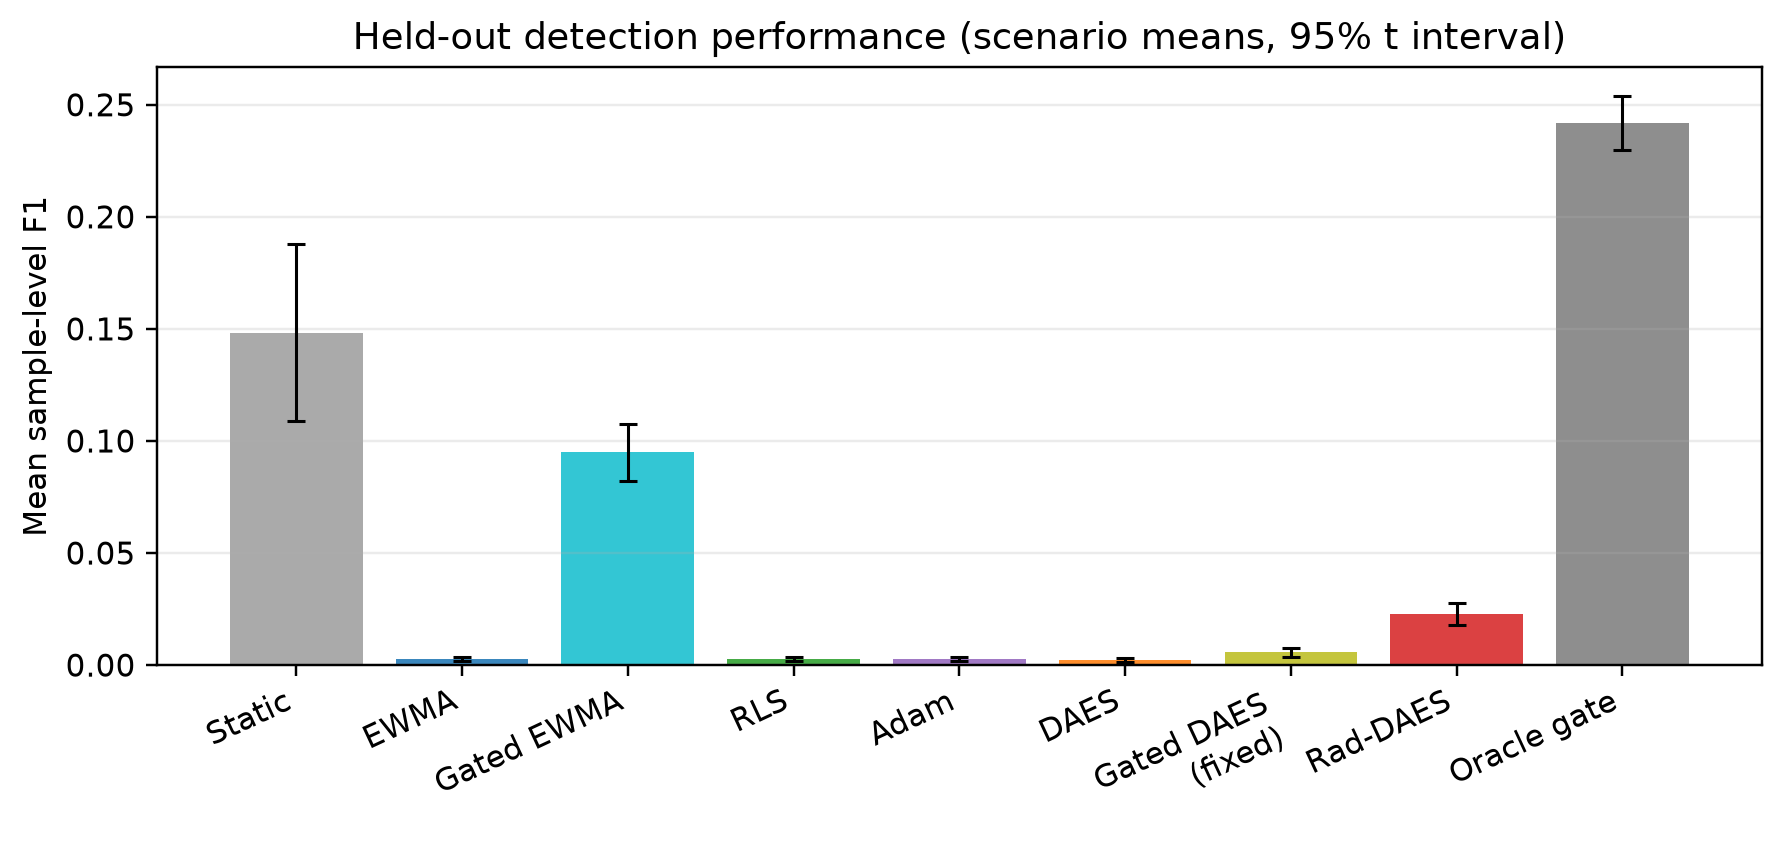
\includegraphics[width=0.92\linewidth]{../results/figures/fig_primary_f1.png}
\caption{Mean sample-level F1 by method. Error bars are 95\% Student-$t$ intervals across the 32 held-out scenario means. The oracle gate is a non-deployable reference.}
\label{fig:primary}
\end{figure}

\paragraph{The operating point dominates the ranking.}
The four methods whose development configurations satisfied the false-alarm constraint (EWMA, RLS, Adam, ungated DAES) have test F1 at most $0.003$ and detect at most 6\% of source events, with test FAR between 2.0 and 2.5/h. They are, in effect, blind at the calibrated operating point. The methods with visible detection either violate the false-alarm constraint or use labels: gated EWMA reaches F1 \GatedEWMAFone{} at \GatedEWMAFarPerHour{}/h, and Rad-DAES reaches \RadDAESFone{} at \RadDAESFarPerHour{}/h. \texttt{static} reaches \StaticFone{} only by alarming on 13.4\% of all samples. There is no deployable method in the matrix that is both sensitive and quiet. Figure~\ref{fig:tradeoff} plots this trade-off directly.

Table~\ref{tab:discrimination} separates threshold choice from separability. The oracle gate has the highest ROC AUC (0.773) and PR AUC (0.223), followed by \texttt{static} (0.728 and 0.128) and gated EWMA (0.691 and 0.089). Rad-DAES obtains ROC AUC \RadDAESRocAuc{} and PR AUC \RadDAESPrAuc{}, below both gated EWMA and \texttt{static}. The ordering is therefore not an artefact of one threshold: the DAES-based methods rank source samples less well than the simpler alternatives on these streams.

\begin{table}[t]
\centering
\caption{Threshold-free discrimination and gate behaviour. ROC/PR AUC use the pre-update score and do not depend on the alarm threshold. Event detection is the fraction of 960 source events with at least one alarm. Alarm fraction is the fraction of all evaluated samples that alarm. Release rate is the fraction of samples in which the sustained-exceedance release is active.}
\label{tab:discrimination}
\scriptsize
\setlength{\tabcolsep}{3pt}
\begin{tabular}{lccccccc}
\toprule
Method & ROC AUC & PR AUC & Event det. & Alarm frac. & Gate rej.\ clean & Gate rej.\ source & Release rate \\
\midrule
Static & 0.728 & 0.128 & 0.821 & 0.1341 & 0.397 & 0.630 & 0.0017 \\
EWMA & 0.622 & 0.031 & 0.060 & 0.0007 & 0.260 & 0.333 & 0.0000 \\
Gated EWMA & 0.691 & 0.089 & 0.406 & 0.0296 & 0.275 & 0.406 & 0.0000 \\
RLS & 0.622 & 0.031 & 0.060 & 0.0007 & 0.260 & 0.333 & 0.0000 \\
Adam & 0.637 & 0.033 & 0.056 & 0.0007 & 0.260 & 0.333 & 0.0000 \\
DAES & 0.600 & 0.024 & 0.054 & 0.0006 & 0.260 & 0.330 & 0.0000 \\
Gated DAES (fixed) & 0.558 & 0.019 & 0.059 & 0.0019 & 0.260 & 0.326 & 0.0000 \\
Rad-DAES & 0.629 & 0.036 & 0.105 & 0.0054 & 0.261 & 0.338 & 0.0000 \\
Oracle gate & 0.773 & 0.223 & 0.736 & 0.0039 & 0.260 & 0.485 & 0.0000 \\
\bottomrule
\end{tabular}

\end{table}

\begin{figure}[t]
\centering
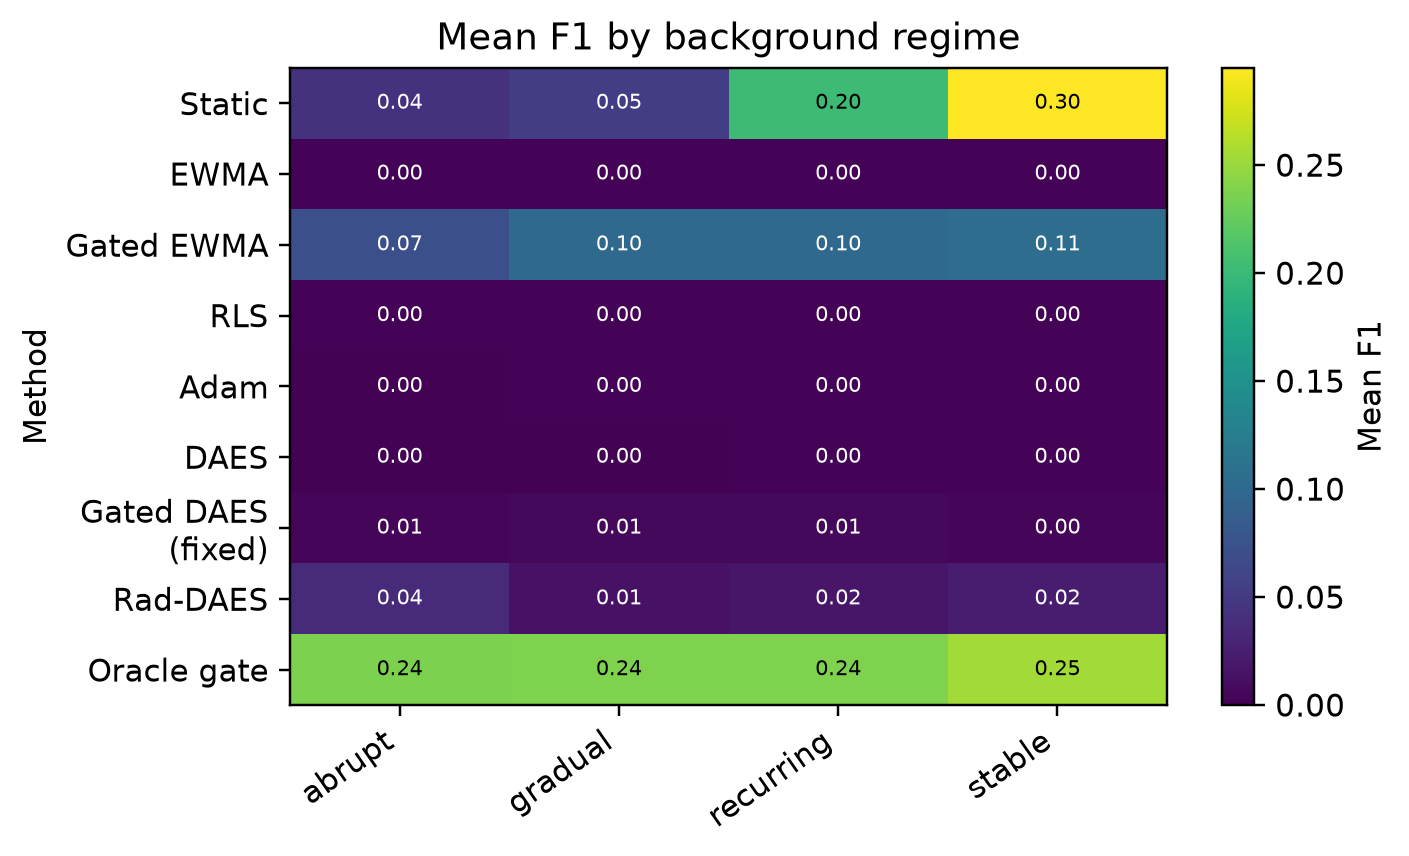
\includegraphics[width=0.92\linewidth]{../results/figures/fig_f1_by_regime.png}
\caption{Mean F1 by background regime. Each cell is the mean over the eight fault conditions and five seeds.}
\label{fig:regime}
\end{figure}

\begin{figure}[t]
\centering
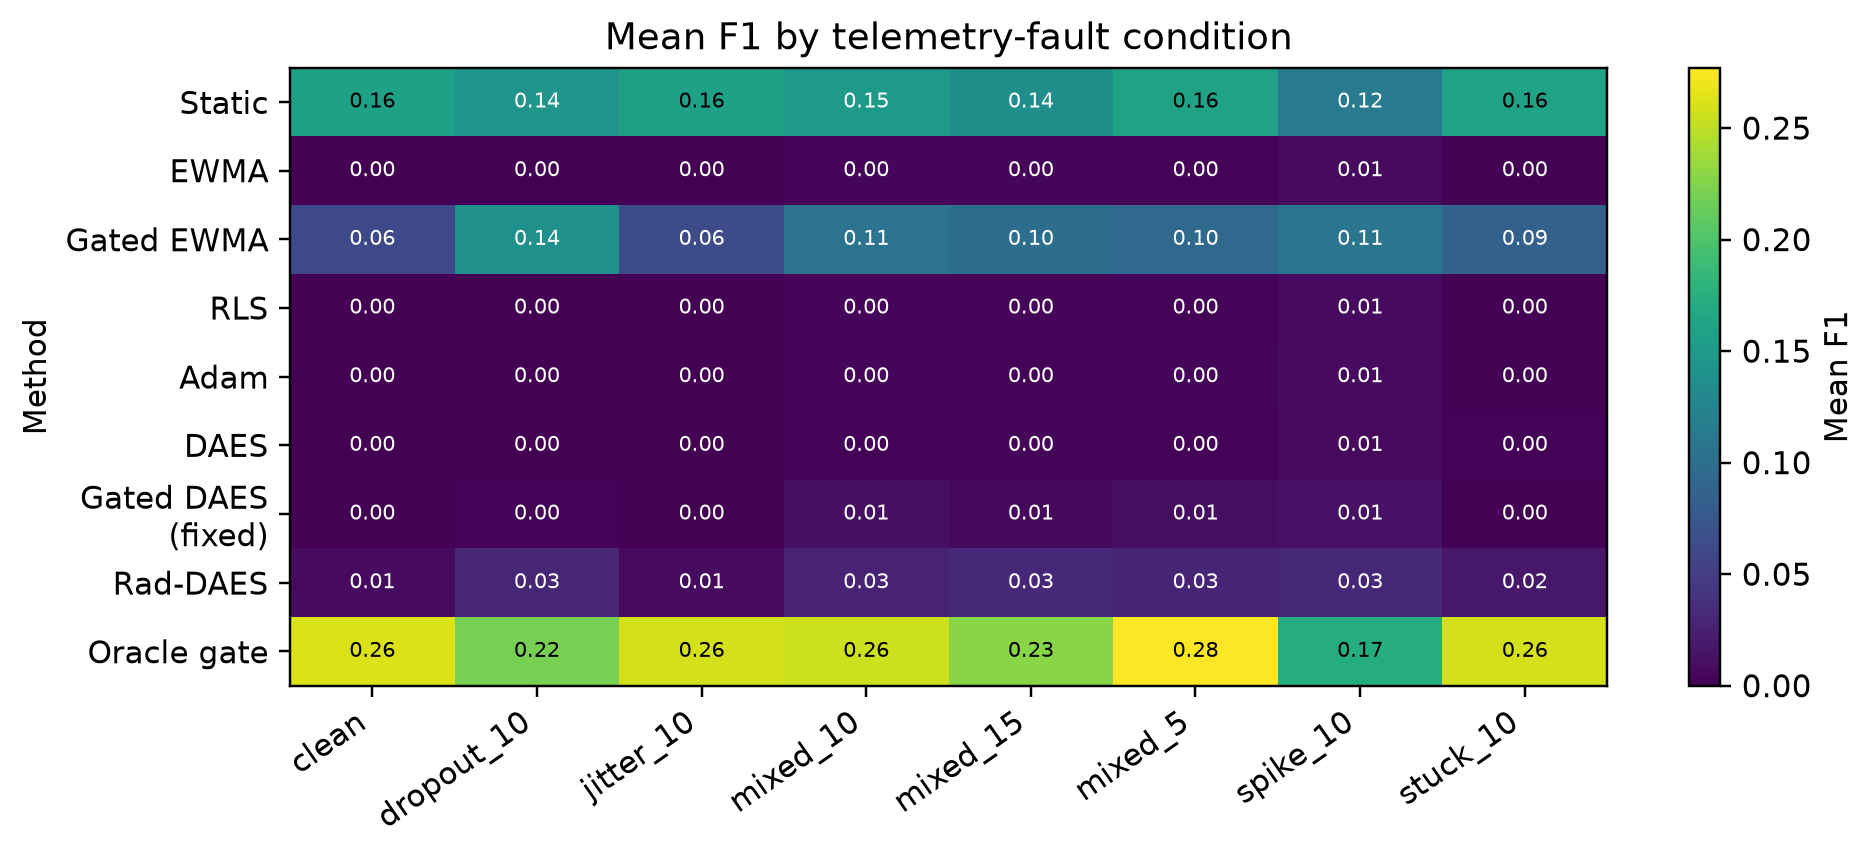
\includegraphics[width=0.98\linewidth]{../results/figures/fig_f1_by_fault.png}
\caption{Mean F1 by telemetry-fault condition. Each cell is the mean over the four regimes and five seeds.}
\label{fig:fault}
\end{figure}

\begin{figure}[t]
\centering
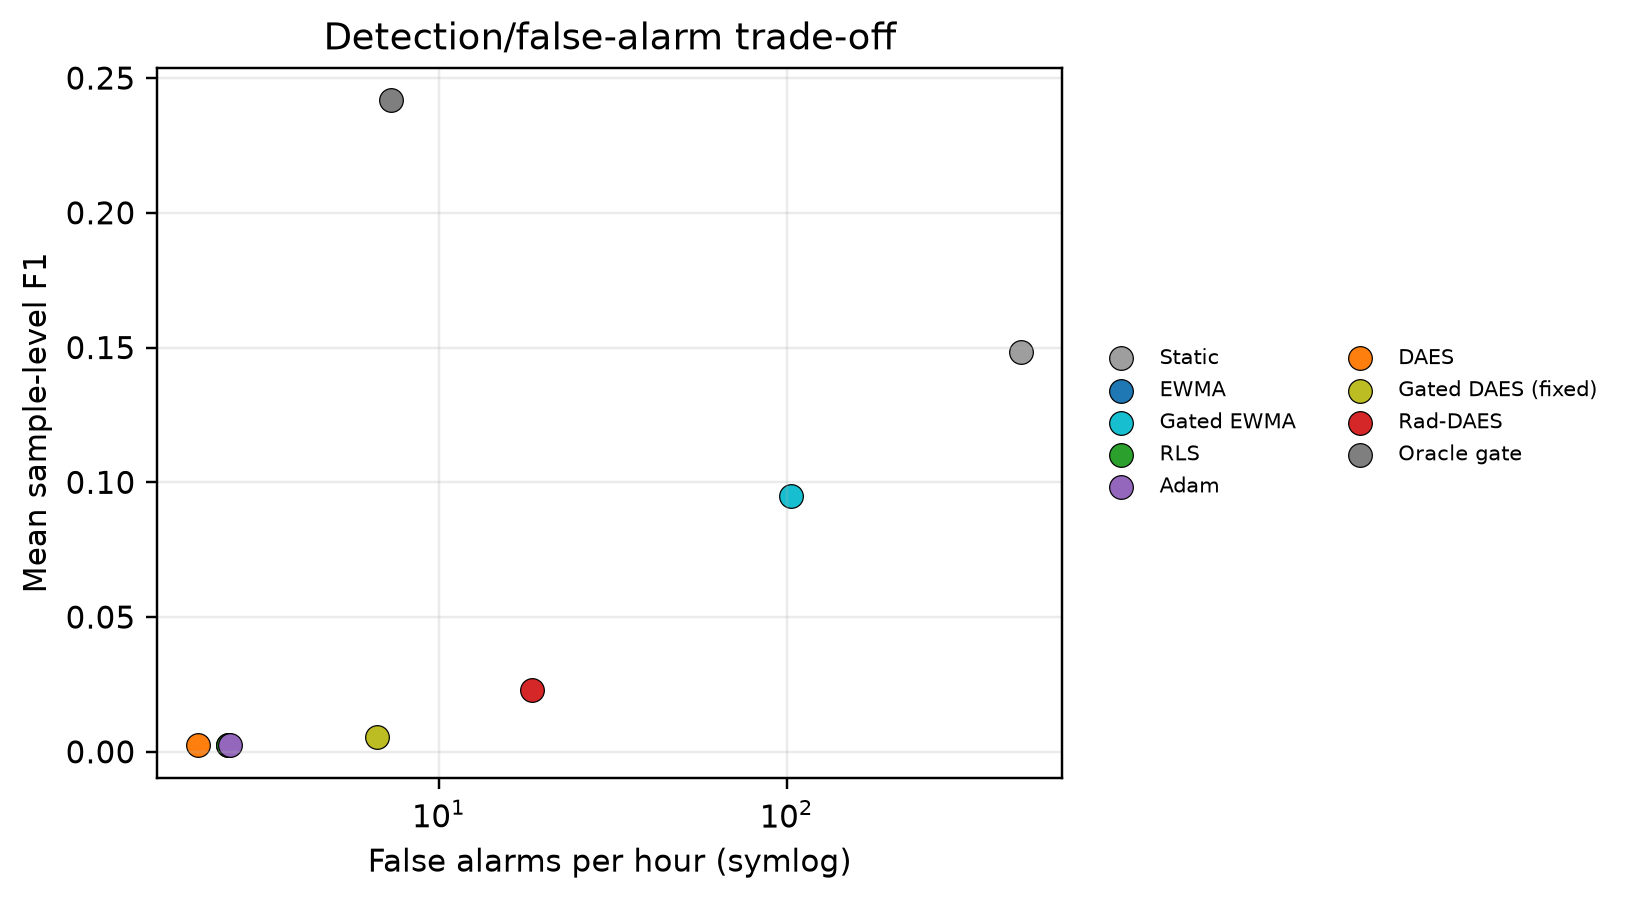
\includegraphics[width=0.78\linewidth]{../results/figures/fig_far_vs_f1.png}
\caption{Detection/false-alarm trade-off. The horizontal axis is symlog because static and some gated configurations produce very large drift-induced false-alarm burdens.}
\label{fig:tradeoff}
\end{figure}

\paragraph{Regime and fault structure.}
Figures~\ref{fig:regime} and~\ref{fig:fault} show that performance is not uniform. The recurring regime is the only regime not used for tuning; it is therefore the clearest check of whether a configuration generalises to a different drift shape. It does not rescue the candidate: Rad-DAES remains below gated EWMA and far below the oracle. Fault conditions change which samples are eligible for updating, so a method that looks adequate on clean streams can lose when dropout, jitter, stuck, or spike faults are present. The spike condition is the worst for false alarms: Rad-DAES reaches \RadDAESFarPerHour{}/h on average but 68.8/h under \texttt{spike\_10}, because a spike both alarms and freezes the update.

\paragraph{Gate behaviour.}
The gate rejects 26.1\% of clean samples and 33.8\% of source samples for Rad-DAES, and the sustained release is active on about $3\times10^{-6}$ of samples. The release is not merely rare: in the representative trace (Figure~\ref{fig:trace}) the consecutive-exceedance counter reaches 89 samples and then resets, one sample short of the 90-sample patience, so the model stays frozen through the step. The tracked mean remains near its pre-step value for roughly 350\,s while the true background has already moved by about 170 counts/s. The gate's source-rejection rate is the expected cost of protecting the background, but here the same mechanism also protects the background from the drift it is supposed to follow. Figure~\ref{fig:gate} summarises the rejection rates by sample type.

\begin{figure}[t]
\centering
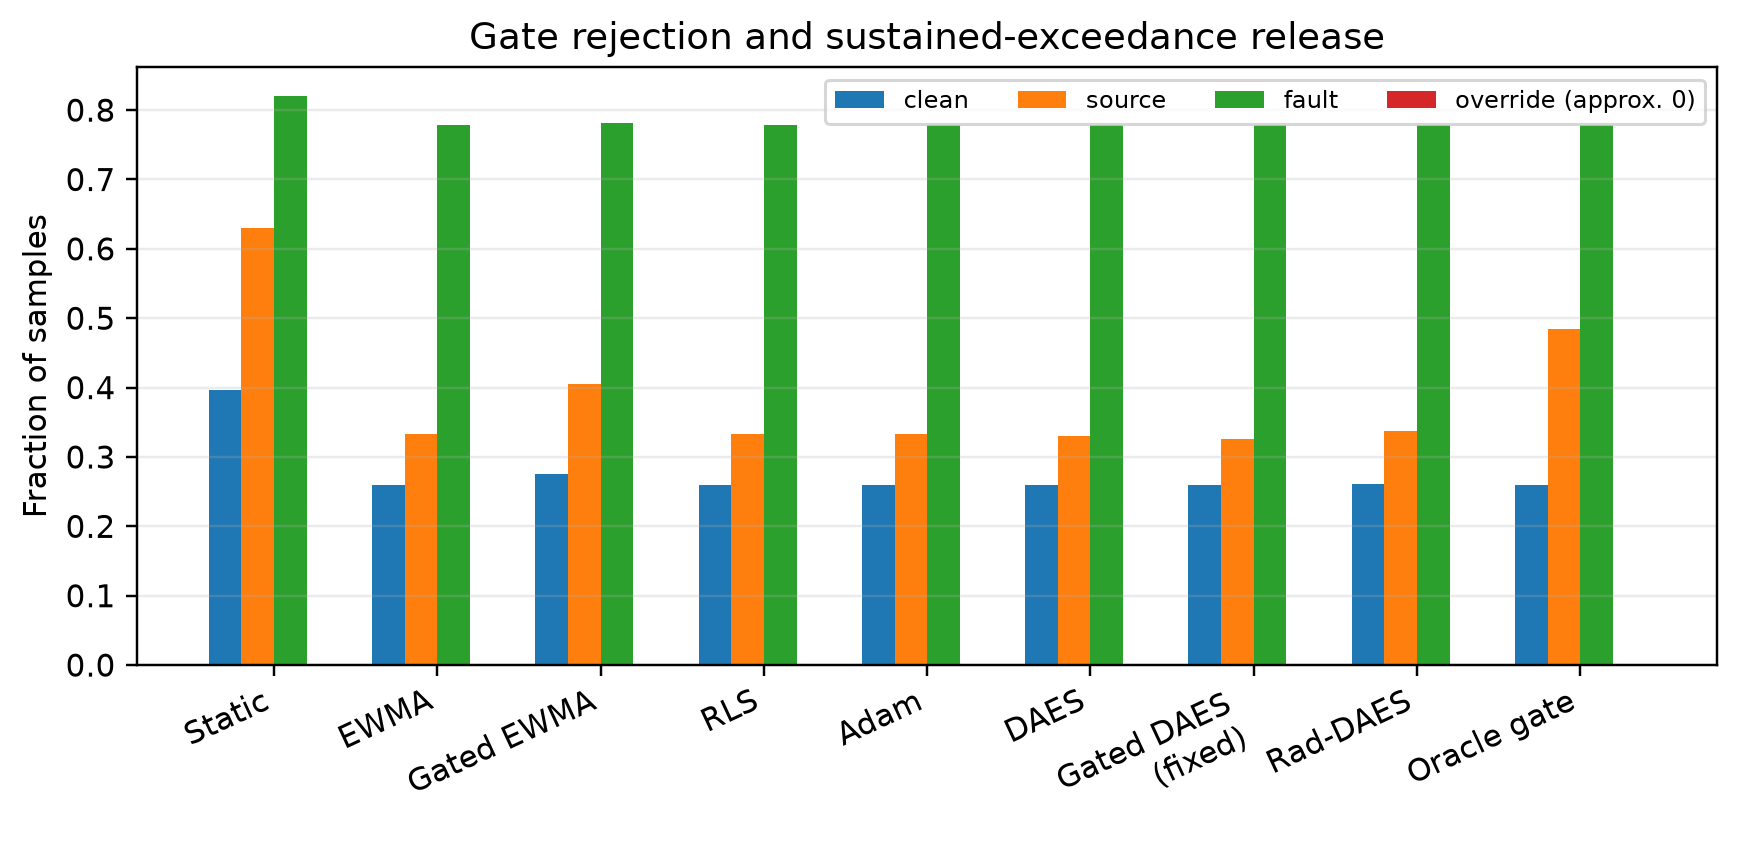
\includegraphics[width=0.92\linewidth]{../results/figures/fig_gate.png}
\caption{Gate rejection rates for clean, source, and fault samples, and the rate of sustained-exceedance release. A high source-rejection rate is the expected cost of protecting the background; it is also a recall risk.}
\label{fig:gate}
\end{figure}

\begin{figure}[t]
\centering
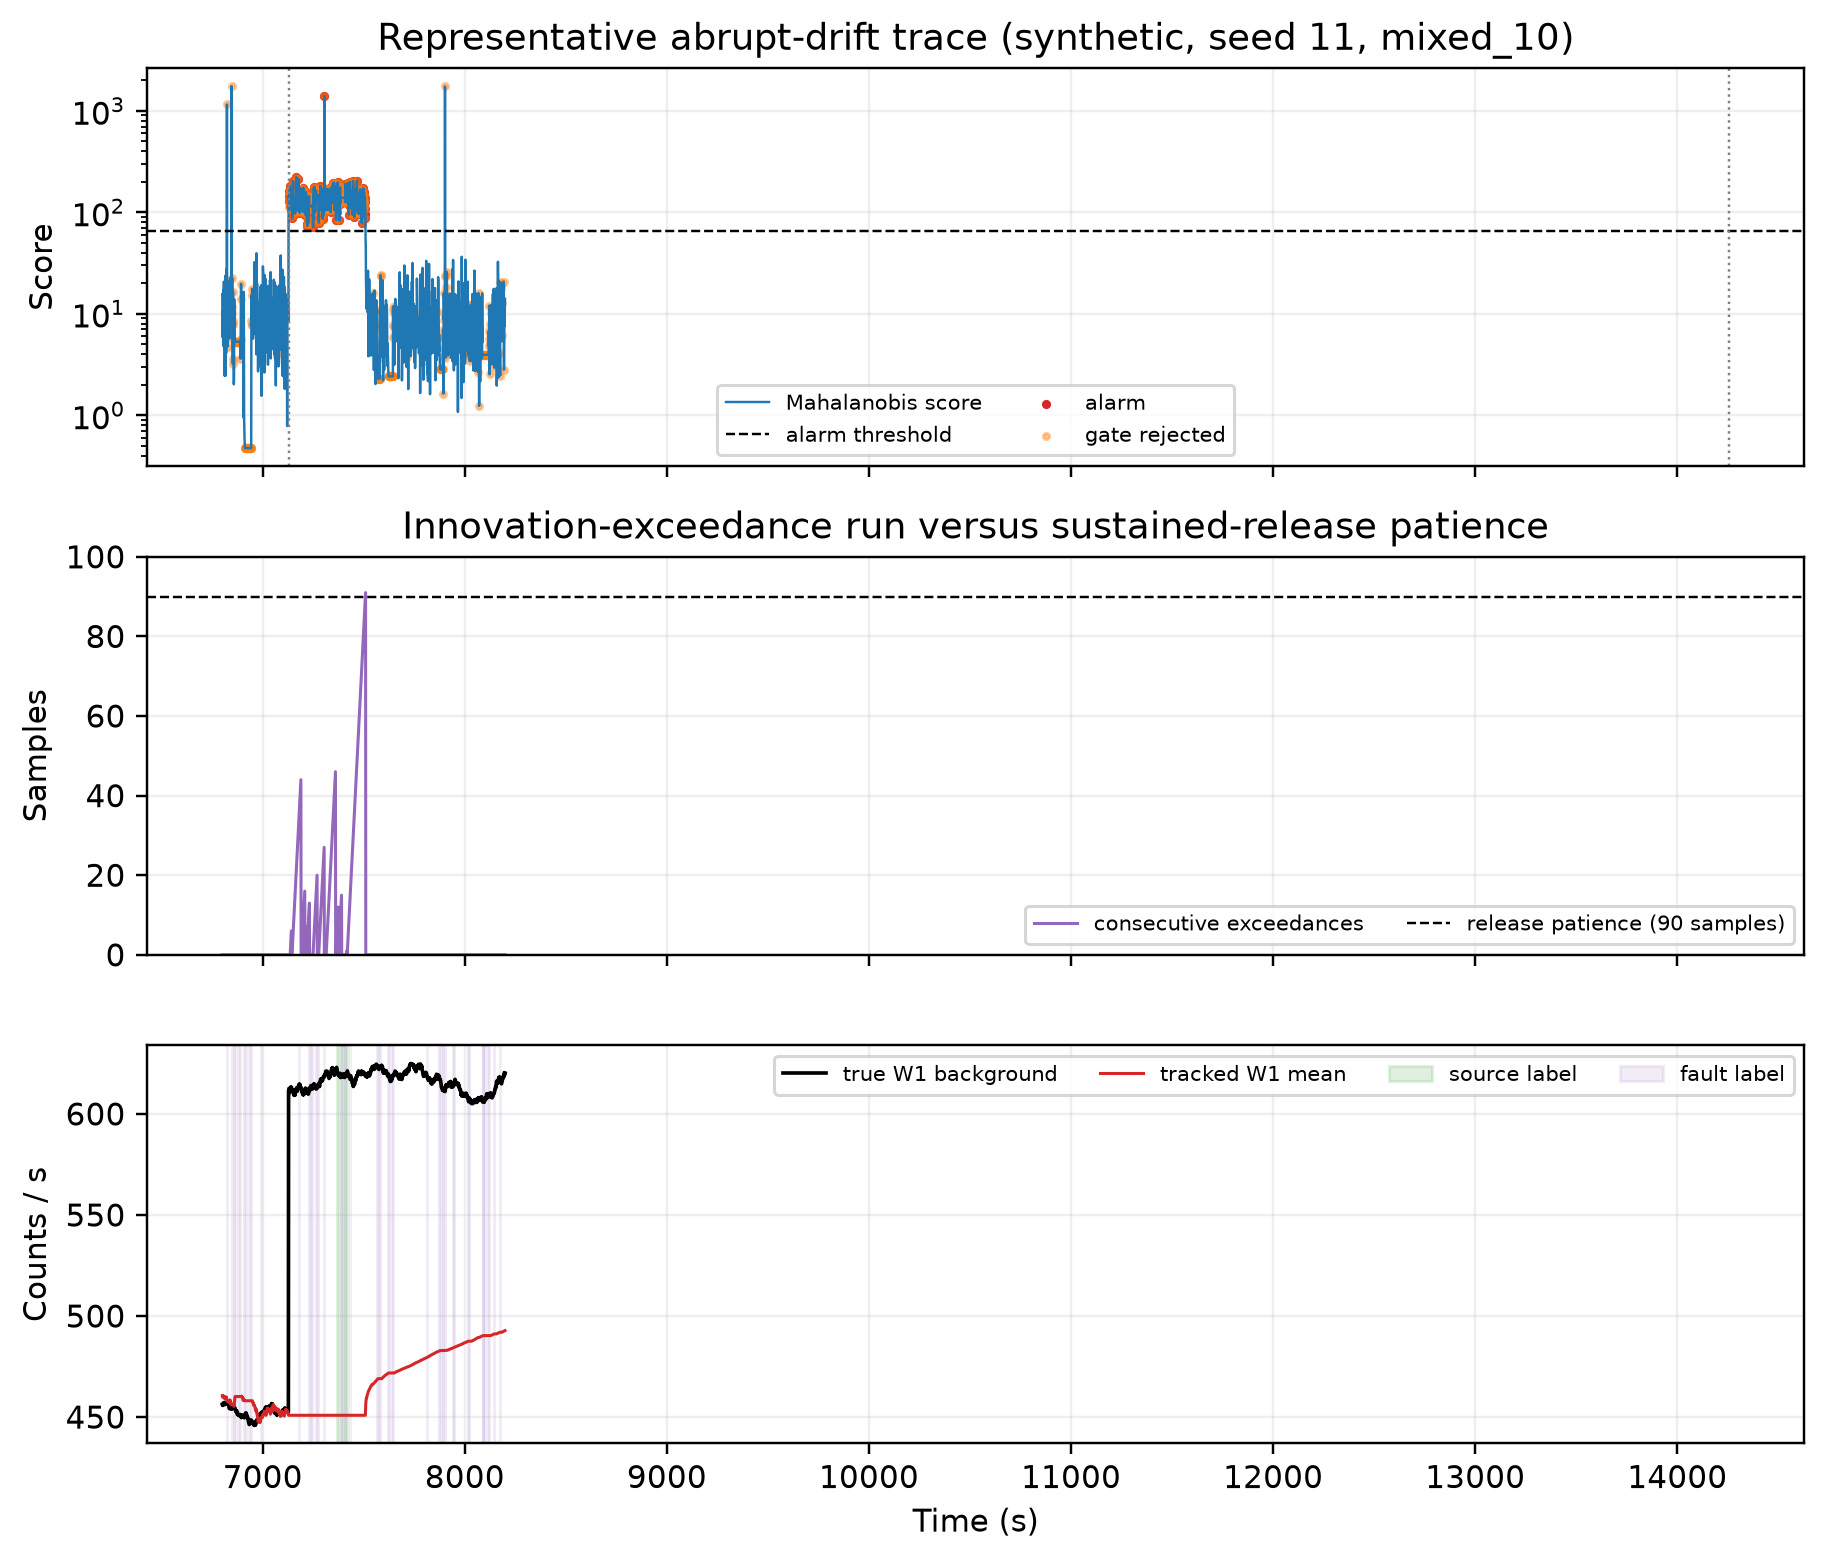
\includegraphics[width=0.95\linewidth]{../results/figures/fig_trace.png}
\caption{Representative abrupt-drift trace for Rad-DAES (synthetic, seed 11, \texttt{mixed\_10}). Top: pre-update score, alarms, and gate rejections. Middle: consecutive innovation exceedances versus the 90-sample release patience; the counter peaks at 89 and resets. Bottom: true and tracked W1 background, with source and fault labels.}
\label{fig:trace}
\end{figure}

\paragraph{Recovery and stability.}
Figure~\ref{fig:recovery} reports recovery time after abrupt steps. Recovery is defined as the first sample at which every window's relative mean error stays below 5\% for 30 consecutive samples; an event that never meets the condition is not silently counted as a success. Rad-DAES recovers 55 of 80 abrupt-step events with a mean recovery time of \RadDAESRecoveryMean{}\,s; gated EWMA recovers all 80 at \GatedEWMARecoveryMean{}\,s but with a much higher false-alarm burden; ungated EWMA and RLS recover all 80 at about 399\,s while remaining nearly blind to sources; \texttt{static} recovers none. Recovery and detection therefore pull in opposite directions in this matrix, and no method achieves both.

\begin{figure}[t]
\centering
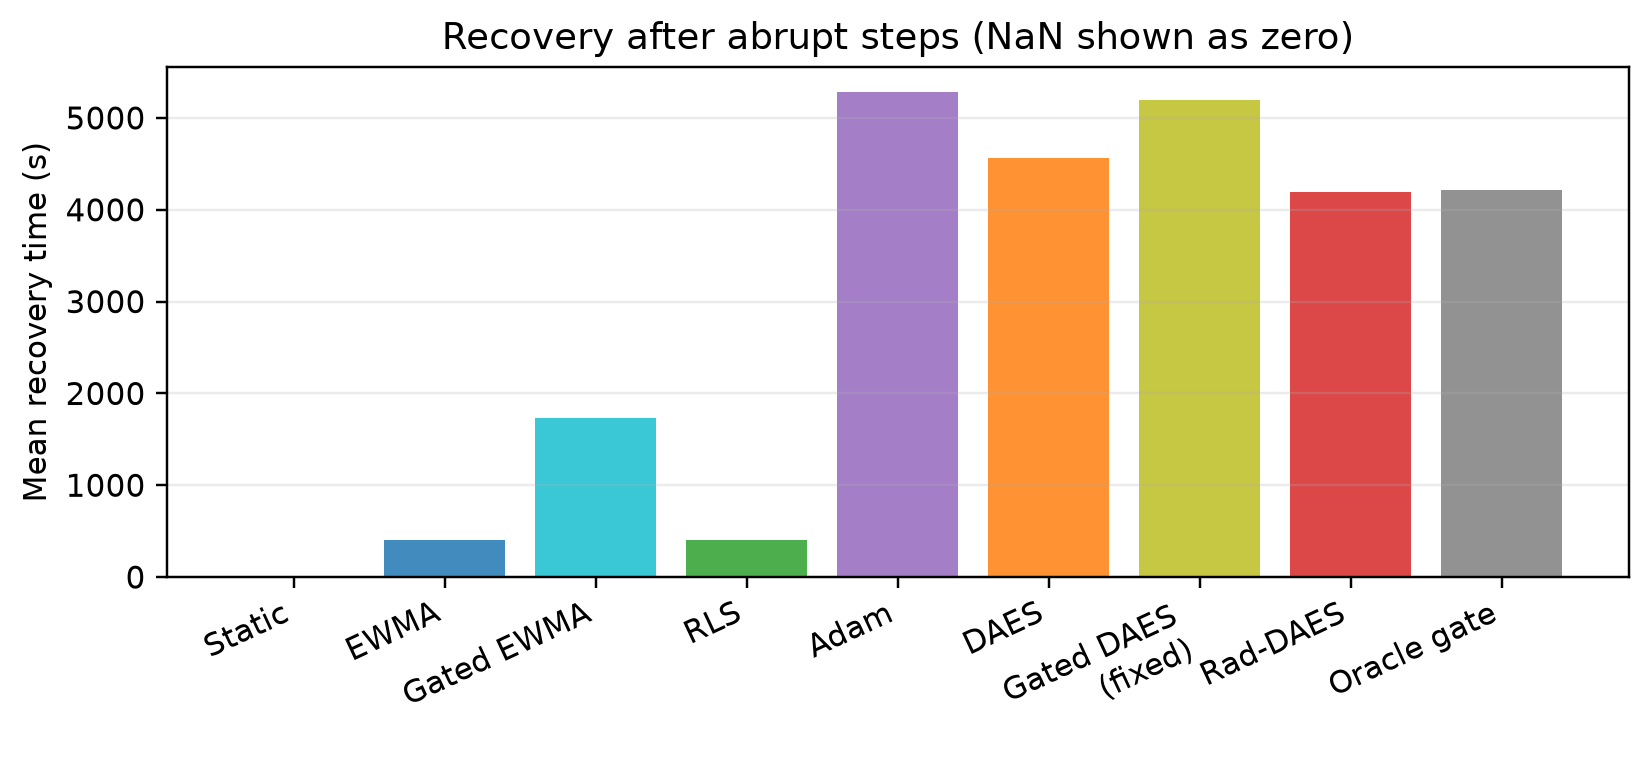
\includegraphics[width=0.78\linewidth]{../results/figures/fig_recovery.png}
\caption{Mean recovery time after abrupt steps. Missing values are shown as zero only for display; they are not treated as recovered in the tables.}
\label{fig:recovery}
\end{figure}

\begin{table}[t]
\centering
\caption{Paired differences (Rad-DAES minus the named method) over matched scenario/seed pairs. Each pair is one held-out run; the 160 pairs are 32 scenarios $\times$ 5 seeds, and the five seeds of a scenario are treated as independent observations, so within-scenario clustering is not modelled. Positive F1 is better; positive FAR and BG are worse. Intervals are descriptive 95\% Student-$t$ intervals and are not multiplicity-corrected.}
\label{tab:paired}
\scriptsize
\begin{tabular}{llccc}
\toprule
Comparison & Metric & Mean difference & 95\% CI & Pairs \\
\midrule
Rad-DAES minus Static & f1 & -0.125 & [-0.146, -0.105] & 160 \\
Rad-DAES minus Static & far\_per\_hour & -453.9 & [-534.8, -372.9] & 160 \\
Rad-DAES minus Static & bg\_rel\_error & -0.029 & [-0.034, -0.024] & 160 \\
Rad-DAES minus EWMA & f1 & 0.020 & [0.013, 0.027] & 160 \\
Rad-DAES minus EWMA & far\_per\_hour & 16.032 & [6.324, 25.741] & 160 \\
Rad-DAES minus EWMA & bg\_rel\_error & 0.010 & [0.008, 0.012] & 160 \\
Rad-DAES minus Gated EWMA & f1 & -0.072 & [-0.081, -0.063] & 160 \\
Rad-DAES minus Gated EWMA & far\_per\_hour & -84.240 & [-122.8, -45.653] & 160 \\
Rad-DAES minus Gated EWMA & bg\_rel\_error & 0.008 & [0.006, 0.010] & 160 \\
Rad-DAES minus RLS & f1 & 0.020 & [0.013, 0.027] & 160 \\
Rad-DAES minus RLS & far\_per\_hour & 16.032 & [6.324, 25.741] & 160 \\
Rad-DAES minus RLS & bg\_rel\_error & 0.010 & [0.008, 0.012] & 160 \\
Rad-DAES minus Adam & f1 & 0.020 & [0.014, 0.027] & 160 \\
Rad-DAES minus Adam & far\_per\_hour & 16.008 & [6.291, 25.726] & 160 \\
Rad-DAES minus Adam & bg\_rel\_error & -0.002 & [-0.004, -0.000] & 160 \\
Rad-DAES minus DAES & f1 & 0.020 & [0.014, 0.027] & 160 \\
Rad-DAES minus DAES & far\_per\_hour & 16.478 & [6.720, 26.236] & 160 \\
Rad-DAES minus DAES & bg\_rel\_error & -0.012 & [-0.017, -0.007] & 160 \\
Rad-DAES minus Gated DAES (fixed) & f1 & 0.017 & [0.011, 0.023] & 160 \\
Rad-DAES minus Gated DAES (fixed) & far\_per\_hour & 11.860 & [2.278, 21.441] & 160 \\
Rad-DAES minus Gated DAES (fixed) & bg\_rel\_error & -0.043 & [-0.044, -0.043] & 160 \\
Rad-DAES minus Oracle gate & f1 & -0.219 & [-0.231, -0.207] & 160 \\
Rad-DAES minus Oracle gate & far\_per\_hour & 11.217 & [1.634, 20.799] & 160 \\
Rad-DAES minus Oracle gate & bg\_rel\_error & 0.011 & [0.010, 0.012] & 160 \\
\bottomrule
\end{tabular}

\end{table}

\paragraph{Tuning and fallbacks.}
Table~\ref{tab:tuning} records the selected development configuration for each method. Four of the nine methods used a fallback, meaning that no candidate met both the background-error and false-alarm constraints on the development scenarios. Rad-DAES selected the largest gain in the grid ($\gamma=0.5$) with a development FAR of 28.6/h, more than fourteen times the constraint; gated EWMA selected the smallest EWMA weight but still had a development FAR of 99.4/h. The oracle gate selected the smallest gain ($\gamma=0.05$) and had a development FAR of 12.5/h. The oracle's advantage is therefore not an isolated gate effect: it combines perfect labelling with a ten-fold gentler step, and the two cannot be separated in this matrix. The selected configurations were frozen before the test matrix.

\begin{table}[t]
\centering
\caption{Selected development configurations and development means. ``Fallback'' means no candidate satisfied both the background-error and false-alarm constraints.}
\label{tab:tuning}
\scriptsize
\begin{tabular}{llcccc}
\toprule
Method & Selected configuration & Status & Dev F1 & Dev BG & Dev FAR/h \\
\midrule
Static & \texttt{default} & fixed & 0.137 & 0.0644 & 647.7 \\
EWMA & \texttt{ewma\_alpha=0.02} & feasible & 0.004 & 0.0136 & 1.11 \\
Gated EWMA & \texttt{ewma\_alpha=0.005;gate\_quantile=0.999} & fallback & 0.078 & 0.0148 & 99.36 \\
RLS & \texttt{rls\_forgetting=0.98} & feasible & 0.004 & 0.0136 & 1.11 \\
Adam & \texttt{adam\_learning\_rate=0.02} & feasible & 0.005 & 0.0261 & 1.09 \\
DAES & \texttt{daes\_gain=0.2} & feasible & 0.004 & 0.0417 & 1.05 \\
Gated DAES (fixed) & \texttt{daes\_gain=0.5;gate\_quantile=0.995} & fallback & 0.011 & 0.0692 & 12.42 \\
Rad-DAES & \texttt{daes\_gain=0.5;gate\_quantile=0.999} & fallback & 0.036 & 0.0257 & 28.64 \\
Oracle gate & \texttt{daes\_gain=0.05} & fallback & 0.228 & 0.0147 & 12.48 \\
\bottomrule
\end{tabular}

\end{table}

\section{Discussion}

The experiment was designed to test a trade-off, not to demonstrate that a new method wins. The answer is negative, and three mechanisms explain most of it.

\emph{First, the innovation guard confuses drift with a source.} A persistent background step produces a sustained score above the gate threshold, so the gate freezes the mean precisely when the mean needs to move. The 90-sample release was intended to break this deadlock, but it requires an uninterrupted run of exceedances; Poisson noise and the oscillating score reset the counter. In the representative trace the counter peaks at 89 and resets. The result is a frozen model, a long alarm burst, and a slow recovery. This is a design failure of the release rule, not a tuning issue: the rule is brittle by construction because it depends on a run length in a noisy sequence.

\emph{Second, the adaptive background appears to absorb source energy.} Both the mean and the covariance update on a 50-sample time constant, comparable to the 20--60\,s source duration. During the ramp of a source event the score is still below the gate threshold, so the gate passes those samples; the mean then moves toward the source and the covariance learns its outer product, and the score for the peak falls. This is consistent with the threshold-free results: \texttt{static}, which updates neither the mean nor the covariance, has ROC AUC 0.728, while the adaptive methods have ROC AUC between 0.558 and 0.691. We did not run a covariance-frozen or mean-frozen ablation, so the two channels are not separated experimentally; the static-versus-adaptive contrast supports the general mechanism, not the share attributable to covariance. It is the most plausible explanation for why the ungated methods detect only about 6\% of events despite a nominal 3--8$\sigma$ source amplitude.

\emph{Third, the selection rule was infeasible.} The development constraint (FAR $\le 2$/h, background error $\le 0.10$) could not be met by any gated configuration under abrupt drift. The fallback rule then chose configurations that violated the FAR constraint by one to two orders of magnitude, and those configurations were frozen for test. The four feasible methods were feasible only because they were nearly blind. The protocol therefore did not compare methods at a common, achievable operating point; it compared blind methods against noisy ones. A matched-FAR evaluation, or a prespecified ROC/PR analysis, would have been more informative. The ROC/PR table is reported here as a secondary analysis, but it was not the basis of the selection rule.

The practical implication is that the three decisions should not share one score. A drift detector, a source detector, and a telemetry-integrity check answer different questions \citep{gama2014survey,isermann2005model}; using the same Mahalanobis score for gating and alarming creates the coupling observed here. A two-timescale covariance (fast for the mean, slow or robust for the detector), or a covariance that is frozen during suspected sources, is a concrete next step. None of these is implemented or validated in this draft.

The draft does not establish that Rad-DAES is novel. The literature review here is structured but not a full systematic review; the closest related work on portal data and concept drift is cited only to frame the problem. A novelty claim would require a protocol-driven review and a direct comparison on public data.

\section{Limitations and threats to validity}

\begin{itemize}
  \item \textbf{No real data.} RADAI requires an account and a large download; PyRIID requires a compatible Python environment and spectra conversion; the JRC reference spectra are not a continuous portal stream. No credentials were used and no real stream was parsed. Gate~1 of the project plan is a partial failure.
  \item \textbf{Synthetic generator.} The regimes, source templates, amplitudes, and fault rates are design choices. They are not fitted to measured background. The Poisson model ignores detector resolution, dead time, and spectrum unfolding \citep{knoll2010radiation}. The $\sin^2$ source profile makes the peak narrow, which penalises sample-level F1; event-level detection is reported to reduce that sensitivity, but it does not eliminate it. The design is reported in the form recommended for simulation studies \citep{morris2019simulation}, but a synthetic study cannot substitute for measured streams.
  \item \textbf{Mechanism inferred, not isolated.} The adaptive-background explanation (mean and covariance) is supported by the static-versus-adaptive contrast and by the saved traces, but no covariance-frozen or mean-frozen ablation was run, so the two channels are not separated. The gate-deadlock explanation is directly visible in one representative trace; the 89-versus-90 near miss is illustrative, not a distributional estimate.
  \item \textbf{Small seed budget.} Five seeds were evaluated per scenario. The primary 95\% confidence intervals are calculated across the 32 scenario means after averaging the five seeds within each scenario. These intervals are descriptive and conditional on the fixed scenario design. They do not quantify uncertainty beyond the selected scenarios or account for model misspecification \citep{greenland2016statistical}.
  \item \textbf{No multiplicity correction.} The scenario-level and paired comparisons are descriptive. A claim of statistical significance is not made, and no false-discovery-rate procedure is applied \citep{benjamini1995controlling}.
  \item \textbf{Design choices.} The 90-sample (90\,s) release, the 0.5--1.5\,s timing bound, the 0.25--3.5 Fano bounds, the 0.25 covariance floor, the 50-sample covariance time constant, and the six windows are choices, not validated constants. Sensitivity analyses are future work.
  \item \textbf{Threshold transfer.} Thresholds calibrated on clean stable streams do not transfer to drift regimes: even the oracle gate has 7.3 false alarms/h on test. The 1/h calibration target is therefore not an operational guarantee, and portal false-alarm testing requires a broader operating-characteristic study than the one reported here \citep{burr2007alarm,leber2020false}.
  \item \textbf{DAES provenance.} The DAES equations follow the supplied scalar reference implementation. The matrix update in some generated planning material is not implemented as DAES. The wrapper's use of a Gaussian quasi-likelihood Hessian is an adaptation, not a theorem.
  \item \textbf{No field readiness.} Runtime is offline Python on synthetic arrays. No hardware latency, network delay, calibration uncertainty, or regulatory requirement is modelled.
\end{itemize}

\section{Reproducibility}

{\sloppy
The repository is self-contained and separate from the unrelated projects that share the workspace. The synthetic generator, gate, DAES controller, background model, detector, runner, tests, scripts, raw CSV files, tables, and figures are included. The packaging follows the reproducibility principle that data, code, and the computational narrative should be inspectable together \citep{peng2011reproducible}. The main commands are:\par}
\begin{verbatim}
python -m pip install -e .
python -m pytest -q
python scripts/run_benchmarks.py --mode full --output results/raw
python scripts/aggregate_results.py
python scripts/make_figures.py
python scripts/audit_results.py
\end{verbatim}
The runner writes a manifest with Python and package versions, configuration hashes, seed lists, and run counts. Every table and figure is generated from saved CSV or trace files; no result is typed into the manuscript by hand. The audit script checks matrix completeness, the frozen selection and thresholds, a determinism spot-check of saved rows, config hashes, and the presence of every table, figure, and macro used here. The original DAES reference file was read from an external snapshot for interface documentation and was not vendored or modified. Its SHA-256 and the archive SHA-256 are recorded in \texttt{docs/daes\_interface.md}.

{\sloppy
The raw run was launched with \texttt{--output results} and then moved into \texttt{results/raw/} to match the layout read by the aggregation and audit scripts; the only edited field was the trace-path column of \texttt{trace\_index.csv}. This is documented in \texttt{results/raw/README.md}.\par}

\section{Conclusion}

This draft delivers a small, complete, reproducible synthetic study of guarded drift-aware background tracking, and its result is negative. Rad-DAES does not improve the detection/false-alarm trade-off on these streams: its F1 is \RadDAESFone{} at \RadDAESFarPerHour{}/h, while the four false-alarm-compliant methods are nearly blind and the non-deployable oracle reaches only \BestValue{}. The traces identify two concrete failure modes, gate-induced freezing under drift and apparent adaptive-background contamination during source ramps, and the development selection rule is shown to be infeasible at the prespecified operating point. The value of the draft is the auditable pipeline and the explicit evidence boundary, not a claim that the candidate method is ready for a portal.

\bibliographystyle{plainnat}
\bibliography{references}

\appendix
\section{Implementation map}

\begin{table}[htbp]
\centering
\caption{Where each component is implemented and tested. Package paths are relative to \texttt{src/rad\_daes/}; script, test, and report paths are relative to the repository root.}
\small
\setlength{\tabcolsep}{4pt}
\begin{tabular}{lll}
\toprule
Component & Source & Test \\
\midrule
Synthetic streams & \texttt{data/synthetic.py} & \texttt{tests/test\_synthetic.py} \\
Window definitions & \texttt{preprocessing/windows.py} & configuration checks \\
Background model & \texttt{background/model.py} & \texttt{tests/test\_background.py} \\
Telemetry gate & \texttt{telemetry/gate.py} & \texttt{tests/test\_gate.py} \\
DAES controller & \texttt{adaptation/daes.py} & \texttt{tests/test\_daes.py} \\
Detector & \texttt{detection/detector.py} & runner integration \\
Metrics & \texttt{evaluation/metrics.py} & \texttt{tests/test\_metrics.py} \\
Runner and calibration & \texttt{evaluation/runner.py} & \texttt{tests/test\_runner.py} \\
Aggregation & \texttt{scripts/aggregate\_results.py} & table checks \\
Audit & \texttt{scripts/audit\_results.py} & \texttt{results/audit\_report.md} \\
\bottomrule
\end{tabular}
\end{table}

\section{Protocol revisions}

The source-placement bug, the sustained-exceedance release, the covariance floor, and the midpoint source profile were fixed on 28 October 2026 before the held-out matrix was run. The revision log is in \texttt{docs/protocol.md}. No held-out result was inspected before these changes. After the frozen test matrix was complete, the threshold-free ROC/PR table and the event-level detection summary were added as secondary analyses; they are computed from columns already saved by the frozen run, and the primary estimand and selection rule were not changed.

\clearpage
\section{Artifact inventory}

Table~\ref{tab:artifacts} lists the paths a reader needs in order to inspect or rerun the study. Counts describe the working repository of 28 October 2026 and exclude Python caches and \LaTeX{} build byproducts; the submission mirror differs only in that the cover-letter DOCX sits at the bundle root, so its \texttt{paper/} directory has six files.

\begin{table}[htbp]
\centering
\caption{Frozen artifact inventory. File counts exclude \texttt{\_\_pycache\_\_} directories.}
\label{tab:artifacts}
\small
\setlength{\tabcolsep}{4pt}
\begin{tabular}{llr}
\toprule
Path & Contents & Files \\
\midrule
\texttt{src/rad\_daes/} & Generator, gate, DAES controller, model, detector, metrics, runner & 16 \\
\texttt{configs/} & Data, model, and experiment configuration & 3 \\
\texttt{tests/} & Unit and integration tests (44 passing) & 7 \\
\texttt{results/raw/} & Calibration, development, and test CSVs; manifest; 4 traces & 13 \\
\texttt{results/tables/} & CSV, \LaTeX{} tables, and generated macros & 16 \\
\texttt{results/figures/} & Seven PNG figures & 7 \\
\texttt{docs/} & Protocol, decisions, DAES interface, results summary, checklist & 8 \\
\texttt{paper/} & Manuscript source, PDF, cover letter, bibliography, supplementary note & 7 \\
\bottomrule
\end{tabular}
\end{table}

The primary test artifact is \texttt{results/raw/test\_runs.csv} (1{,}440 rows). The audit report is regenerated by \texttt{scripts/audit\_results.py} and records 22 checks. No real radiation data are included, because none were obtained (Section~6).

\end{document}
"
\providecommand{\PaperSize}{letterpaper}
\usepackage[\PaperSize,margin=1in]{geometry}
\usepackage{amsmath,amssymb}
\usepackage{booktabs}
\usepackage{graphicx}
\usepackage{siunitx}
\usepackage[hidelinks]{hyperref}
\usepackage[numbers,sort]{natbib}
\usepackage{xcolor}
\usepackage{caption}
\usepackage{subcaption}

\hypersetup{
  pdftitle={Guarded Drift-Aware Background Tracking for Synthetic Radiation-Portal Count Streams: A Reproducible Benchmark and a Negative Result},
  pdfauthor={Tripti Kumari, Chayan Ojha, Mriganko Dey, Ankita Polley},
  pdfsubject={B.Tech group project, Department of Computer Science and Engineering (AI \& ML), Narula Institute of Technology, Agarpara}
}

% Generated by scripts/aggregate_results.py. Do not edit by hand.
\newcommand{\StaticFone}{0.148}
\newcommand{\StaticFarPerHour}{472.4}
\newcommand{\StaticBgRelError}{0.055}
\newcommand{\StaticRecall}{0.370}
\newcommand{\StaticPrecision}{0.249}
\newcommand{\StaticRecoveryMean}{---}
\newcommand{\EWMAFone}{0.003}
\newcommand{\EWMAFarPerHour}{2.476}
\newcommand{\EWMABgRelError}{0.015}
\newcommand{\EWMARecall}{0.002}
\newcommand{\EWMAPrecision}{0.089}
\newcommand{\EWMARecoveryMean}{399.1}
\newcommand{\GatedEWMAFone}{0.095}
\newcommand{\GatedEWMAFarPerHour}{102.7}
\newcommand{\GatedEWMABgRelError}{0.017}
\newcommand{\GatedEWMARecall}{0.121}
\newcommand{\GatedEWMAPrecision}{0.473}
\newcommand{\GatedEWMARecoveryMean}{1734}
\newcommand{\RLSFone}{0.003}
\newcommand{\RLSFarPerHour}{2.476}
\newcommand{\RLSBgRelError}{0.015}
\newcommand{\RLSRecall}{0.002}
\newcommand{\RLSPrecision}{0.089}
\newcommand{\RLSRecoveryMean}{399.1}
\newcommand{\AdamFone}{0.003}
\newcommand{\AdamFarPerHour}{2.500}
\newcommand{\AdamBgRelError}{0.028}
\newcommand{\AdamRecall}{0.002}
\newcommand{\AdamPrecision}{0.078}
\newcommand{\AdamRecoveryMean}{5286}
\newcommand{\DAESFone}{0.002}
\newcommand{\DAESFarPerHour}{2.031}
\newcommand{\DAESBgRelError}{0.038}
\newcommand{\DAESRecall}{0.001}
\newcommand{\DAESPrecision}{0.054}
\newcommand{\DAESRecoveryMean}{4564}
\newcommand{\GatedDAESFixedFone}{0.006}
\newcommand{\GatedDAESFixedFarPerHour}{6.649}
\newcommand{\GatedDAESFixedBgRelError}{0.069}
\newcommand{\GatedDAESFixedRecall}{0.004}
\newcommand{\GatedDAESFixedPrecision}{0.054}
\newcommand{\GatedDAESFixedRecoveryMean}{5196}
\newcommand{\RadDAESFone}{0.023}
\newcommand{\RadDAESFarPerHour}{18.508}
\newcommand{\RadDAESBgRelError}{0.025}
\newcommand{\RadDAESRecall}{0.024}
\newcommand{\RadDAESPrecision}{0.142}
\newcommand{\RadDAESRecoveryMean}{4198}
\newcommand{\OracleGateFone}{0.242}
\newcommand{\OracleGateFarPerHour}{7.292}
\newcommand{\OracleGateBgRelError}{0.014}
\newcommand{\OracleGateRecall}{0.158}
\newcommand{\OracleGatePrecision}{0.721}
\newcommand{\OracleGateRecoveryMean}{4213}
\newcommand{\BestMethod}{Oracle gate}
\newcommand{\BestValue}{0.242}
\newcommand{\NScenarios}{32}
\newcommand{\StaticRocAuc}{0.728}
\newcommand{\StaticPrAuc}{0.128}
\newcommand{\StaticEventDetection}{0.821}
\newcommand{\StaticAlarmFraction}{0.134}
\newcommand{\StaticGateRejectClean}{0.397}
\newcommand{\StaticGateRejectSource}{0.630}
\newcommand{\StaticGateOverrideRate}{0.002}
\newcommand{\EWMARocAuc}{0.622}
\newcommand{\EWMAPrAuc}{0.031}
\newcommand{\EWMAEventDetection}{0.060}
\newcommand{\EWMAAlarmFraction}{0.001}
\newcommand{\EWMAGateRejectClean}{0.260}
\newcommand{\EWMAGateRejectSource}{0.333}
\newcommand{\EWMAGateOverrideRate}{0.000}
\newcommand{\GatedEWMARocAuc}{0.691}
\newcommand{\GatedEWMAPrAuc}{0.089}
\newcommand{\GatedEWMAEventDetection}{0.406}
\newcommand{\GatedEWMAAlarmFraction}{0.030}
\newcommand{\GatedEWMAGateRejectClean}{0.275}
\newcommand{\GatedEWMAGateRejectSource}{0.406}
\newcommand{\GatedEWMAGateOverrideRate}{0.000}
\newcommand{\RLSRocAuc}{0.622}
\newcommand{\RLSPrAuc}{0.031}
\newcommand{\RLSEventDetection}{0.060}
\newcommand{\RLSAlarmFraction}{0.001}
\newcommand{\RLSGateRejectClean}{0.260}
\newcommand{\RLSGateRejectSource}{0.333}
\newcommand{\RLSGateOverrideRate}{0.000}
\newcommand{\AdamRocAuc}{0.637}
\newcommand{\AdamPrAuc}{0.033}
\newcommand{\AdamEventDetection}{0.056}
\newcommand{\AdamAlarmFraction}{0.001}
\newcommand{\AdamGateRejectClean}{0.260}
\newcommand{\AdamGateRejectSource}{0.333}
\newcommand{\AdamGateOverrideRate}{0.000}
\newcommand{\DAESRocAuc}{0.600}
\newcommand{\DAESPrAuc}{0.024}
\newcommand{\DAESEventDetection}{0.054}
\newcommand{\DAESAlarmFraction}{0.001}
\newcommand{\DAESGateRejectClean}{0.260}
\newcommand{\DAESGateRejectSource}{0.330}
\newcommand{\DAESGateOverrideRate}{0.000}
\newcommand{\GatedDAESFixedRocAuc}{0.558}
\newcommand{\GatedDAESFixedPrAuc}{0.019}
\newcommand{\GatedDAESFixedEventDetection}{0.059}
\newcommand{\GatedDAESFixedAlarmFraction}{0.002}
\newcommand{\GatedDAESFixedGateRejectClean}{0.260}
\newcommand{\GatedDAESFixedGateRejectSource}{0.326}
\newcommand{\GatedDAESFixedGateOverrideRate}{0.000}
\newcommand{\RadDAESRocAuc}{0.629}
\newcommand{\RadDAESPrAuc}{0.036}
\newcommand{\RadDAESEventDetection}{0.105}
\newcommand{\RadDAESAlarmFraction}{0.005}
\newcommand{\RadDAESGateRejectClean}{0.261}
\newcommand{\RadDAESGateRejectSource}{0.338}
\newcommand{\RadDAESGateOverrideRate}{0.000}
\newcommand{\OracleGateRocAuc}{0.773}
\newcommand{\OracleGatePrAuc}{0.223}
\newcommand{\OracleGateEventDetection}{0.736}
\newcommand{\OracleGateAlarmFraction}{0.004}
\newcommand{\OracleGateGateRejectClean}{0.260}
\newcommand{\OracleGateGateRejectSource}{0.485}
\newcommand{\OracleGateGateOverrideRate}{0.000}
\newcommand{\PairedStaticFone}{-0.125}
\newcommand{\PairedStaticFarPerHour}{-453.9}
\newcommand{\PairedStaticBgRelError}{-0.029}
\newcommand{\PairedEWMAFone}{0.020}
\newcommand{\PairedEWMAFarPerHour}{16.032}
\newcommand{\PairedEWMABgRelError}{0.010}
\newcommand{\PairedGatedEWMAFone}{-0.072}
\newcommand{\PairedGatedEWMAFarPerHour}{-84.240}
\newcommand{\PairedGatedEWMABgRelError}{0.008}
\newcommand{\PairedRLSFone}{0.020}
\newcommand{\PairedRLSFarPerHour}{16.032}
\newcommand{\PairedRLSBgRelError}{0.010}
\newcommand{\PairedAdamFone}{0.020}
\newcommand{\PairedAdamFarPerHour}{16.008}
\newcommand{\PairedAdamBgRelError}{-0.002}
\newcommand{\PairedDAESFone}{0.020}
\newcommand{\PairedDAESFarPerHour}{16.478}
\newcommand{\PairedDAESBgRelError}{-0.012}
\newcommand{\PairedGatedDAESFixedFone}{0.017}
\newcommand{\PairedGatedDAESFixedFarPerHour}{11.860}
\newcommand{\PairedGatedDAESFixedBgRelError}{-0.043}
\newcommand{\PairedOracleGateFone}{-0.219}
\newcommand{\PairedOracleGateFarPerHour}{11.217}
\newcommand{\PairedOracleGateBgRelError}{0.011}


\title{Guarded Drift-Aware Background Tracking for Synthetic Radiation-Portal Count Streams:\\A Reproducible Benchmark and a Negative Result}
\author{%
  Tripti Kumari\\
  Chayan Ojha\\
  Mriganko Dey\\
  Ankita Polley\\[0.8em]
  \small Department of Computer Science and Engineering (AI \& ML)\\
  \small Narula Institute of Technology, Agarpara, West Bengal\\
  \small B.Tech in Computer Science and Engineering (Artificial Intelligence and Machine Learning)\\
  \small Academic year 2026--2027 (provisional)
}
\date{28 October 2026}

\begin{document}
\maketitle

\begin{abstract}
Radiation-portal monitors must separate source-like count excursions from a drifting background and from telemetry faults. This draft evaluates \emph{Rad-DAES}, a candidate pipeline that combines a four-condition telemetry-integrity gate, a pre-update Mahalanobis detector, and the scalar drift-aware step size of the supplied DAES reference implementation. The study is synthetic-only and deliberately narrow: six-window Poisson streams under four background regimes and eight telemetry-fault conditions, tuned on development seeds only, with the recurring regime held out, and evaluated on \NScenarios{} scenarios with five seeds and nine methods (1{,}440 runs). The result is negative. No deployable method achieved both useful event detection and an acceptable false-alarm rate. The best mean sample-level F1 is \BestValue{} for the non-deployable oracle gate; Rad-DAES obtains \RadDAESFone{} with \RadDAESFarPerHour{} false alarms per hour, and the four methods whose development configurations met the false-alarm constraint obtain F1 at most $0.003$ and detect at most 6\% of source events. The traces show why: after an abrupt background step the innovation guard freezes the model for hundreds of seconds, the 90-sample sustained-release rule almost never fires for Rad-DAES (below 0.01\% of its samples), and the saved traces and static-versus-adaptive comparison are consistent with the adaptive background absorbing source energy during event ramps, although this mechanism was not isolated experimentally. These are simulation results from an unvalidated generator. They do not establish field readiness, operational safety, or novelty, and no statistical-significance claim is made.
\end{abstract}

\section{Introduction}

A radiation portal monitor observes a stream of gamma counts in several energy windows \citep{knoll2010radiation,runkle2009photon}. A source that passes through the portal raises some windows for a short interval; background radon, weather, cargo, and detector drift change the same windows over minutes or hours \citep{sim2021background,sim2024cargo}; and a telemetry fault can make an observation invalid, late, stuck, or implausibly dispersed \citep{isermann2005model,little2019missing}. A background tracker that adapts too eagerly can absorb the source it is meant to detect. A tracker that adapts too slowly leaves a drift-induced residual that looks like a source. The engineering problem is therefore a coupling between detection, adaptation, and data quality, not a standalone optimizer problem.

This draft asks a narrow question: under matched synthetic streams, does a guarded DAES pipeline improve the detection/false-alarm/stability trade-off relative to static, EWMA, gated EWMA, RLS, Adam, ungated DAES, fixed-step gated DAES, and an oracle gate? The answer reported here is no, and the more useful output is a reproducible account of why. The DAES component is the original scalar step-size heuristic supplied with the project brief. The matrix update that appears in some generated planning material is explicitly not implemented as DAES; the discrepancy is documented in the repository.

The paper makes four bounded contributions:
\begin{enumerate}
  \item a reproducible synthetic benchmark with labelled background regimes, source events, and telemetry faults, including a held-out recurring regime;
  \item a documented separation between the original DAES scalar controller, the Gaussian quasi-likelihood curvature used by the wrapper, and the telemetry gate;
  \item a complete negative-and-mixed report: all methods and scenarios are reported, including the cases where the candidate loses;
  \item a mechanistic account, supported by saved per-step traces, of two failure modes: gate-induced freezing under drift and apparent adaptive-background contamination during source ramps.
\end{enumerate}

No real radiation data are used. The data-access blockers are recorded in the repository. The experiments are a first draft, not a field validation.

\section{Related work}

\paragraph{Background estimation and source detection.}
Radiation-portal analysis has moved toward large, realistic datasets and reproducible algorithm development \citep{ghawaly2020data,ghawaly2026radai}. Detection methods range from moving-source algorithms over portal networks \citep{coulon2014moving} to studies of cargo-induced background suppression \citep{sim2024cargo}, standardised portal controls and readouts \citep{tinker2010standardisation}, and standardised data formats \citep{bae2025format}. Reviews of portal detection technology emphasise the low signal-to-background regime and the operational cost of nuisance alarms \citep{runkle2009photon}, while Monte Carlo studies show that background composition and shielding change the observed count distribution \citep{sim2021background}. These works motivate the six-window count representation and the concern with background drift, but they do not provide a local stream on which the present pipeline can be validated. The synthetic generator is therefore an explicit placeholder.

\paragraph{Drift, smoothing, and change detection.}
Concept-drift adaptation distinguishes transient noise, gradual change, abrupt change, and recurring change \citep{gama2014survey}. Non-stationary time-series models make the same point formally: a process whose parameters change over time cannot be summarised by a single stationary model \citep{dahlhaus1997fitting}. The EWMA control chart \citep{roberts1959control}, its broader exponential-smoothing formulation \citep{gardner1985exponential}, and the CUSUM procedure \citep{page1954continuous} are classical tools for the same problem. The gate in this draft uses a sliding-window dispersion check and an innovation threshold rather than a full CUSUM, but the design tension is the same: a persistent shift should eventually be tracked, while a short source-like excursion should not contaminate the background.

\paragraph{Multivariate anomaly detection.}
The Mahalanobis distance provides a scale-free multivariate score that accounts for covariance \citep{mahalanobis1936distance}, and anomaly-detection surveys place covariance-based scoring among the classical statistical approaches \citep{chandola2009anomaly}. The detector in this draft uses that score on a pre-update innovation, so the covariance estimate directly controls both sensitivity and the false-alarm rate. This is a modelling choice, not a claim that the synthetic streams satisfy the Gaussian assumptions under which the score is usually derived.

\paragraph{Detection thresholds and false alarms.}
The Neyman--Pearson criterion formalises the trade-off between detection probability and false-alarm probability \citep{neyman1933problem}. Radiation-portal practice treats alarm criteria and false-alarm testing as first-class design problems rather than afterthoughts \citep{burr2007alarm,leber2020false}, and ROC analysis is the standard way to report threshold-free discrimination \citep{fawcett2006roc}. These sources motivate the two reporting layers used here: a calibrated operating point for the primary comparison, and a threshold-free ROC/PR analysis as a secondary check.

\paragraph{Step sizes and robust estimation.}
Polyak-style gradient methods and two-point step-size rules provide the optimisation background for adaptive step sizes \citep{barzilai1988two,polyak1963gradient}. The supplied DAES implementation is a scalar heuristic in this family: it estimates the largest curvature eigenvalue with power iteration and scales the step by its inverse. Robust location estimation \citep{huber1964robust} and model-based fault diagnosis \citep{isermann2005model} motivate the separation between an outlier-resistant update and a fault detector. Adam \citep{kingma2015adam} and recursive least squares \citep{ljung1999system} are included as optimisation/estimation baselines, not as claims about radiation physics.

\section{Methods}

\subsection{Synthetic streams}

Each stream is a sequence of $D=6$ non-negative count vectors at 1\,Hz. The six energy windows and nominal count rates are design choices taken from the project brief, not calibrated detector properties. Counts are modelled as Poisson variates, the standard first-order description of counting statistics \citep{knoll2010radiation}. For window $j$ and time $t$,
\begin{equation}
  x_{t,j} \sim \mathrm{Poisson}\bigl(\mu^{\mathrm{true}}_{t,j} + s_{t,j}\bigr),
\end{equation}
where $\mu^{\mathrm{true}}_{t}$ is a labelled background mean and $s_{t}$ is a labelled source excess. Poisson draws are made after the background and source terms are combined. Telemetry faults are applied afterwards.

The background regimes are:
\begin{itemize}
  \item \texttt{stable}: a small AR(1) fluctuation around the nominal rate;
  \item \texttt{gradual}: a slow sinusoidal trend plus a linear trend;
  \item \texttt{abrupt}: two multiplicative step changes with different per-window factors;
  \item \texttt{recurring}: three broad bumps, strongest in the low- and high-energy windows.
\end{itemize}
The recurring regime is held out from tuning. Each 6\,h stream attempts six source events of 20--60\,s, with amplitudes 3--8 baseline standard deviations and three templates. The excess follows a $\sin^2$ profile, so a labelled event has low amplitude at both ends and a narrow peak. Fault conditions are \texttt{clean}, \texttt{mixed\_5}, \texttt{mixed\_10}, \texttt{mixed\_15}, and single-mode \texttt{dropout\_10}, \texttt{jitter\_10}, \texttt{stuck\_10}, and \texttt{spike\_10}; the suffix is the approximate fraction of affected samples. The generator, labels, and seeds are deterministic. The design follows the reporting principles for simulation studies: the data-generating mechanism, the tuning rule, and the evaluation estimands are fixed before the held-out matrix is examined \citep{morris2019simulation}.

\subsection{Background model and detector}

The background state is a mean $\mu_t$ and covariance $\Sigma_t$. Detection uses the pre-update innovation
\begin{equation}
  r_t = x_t - \mu_{t-1}, \qquad
  s_t = r_t^\top \bigl(\Sigma_{t-1} + \epsilon I\bigr)^{-1} r_t,
  \label{eq:score}
\end{equation}
with $\epsilon=10^{-6}$. The quadratic form is the Mahalanobis score \citep{mahalanobis1936distance}, used here as a multivariate monitoring statistic. An alarm requires two consecutive scores above a calibrated threshold $\tau_{\mathrm{alarm}}$. The detector never sees the updated background for the current sample: detection precedes adaptation. The detector is evaluated on every sample, including samples that the telemetry gate rejects for updating; a high score can therefore alarm and freeze the model at the same time.

The Gaussian quasi-likelihood
\begin{equation}
  L_t(\theta) = \tfrac12 (x_t-\theta)^\top \Sigma_{t-1}^{-1}(x_t-\theta)
\end{equation}
has gradient $-\Sigma_{t-1}^{-1}r_t$ and Hessian $H_t=\Sigma_{t-1}^{-1}$, the local quadratic model used by Gaussian state estimation \citep{ljung1999system}. The covariance is tracked separately. On an eligible sample, with post-update residual $u_t=x_t-\mu_t$,
\begin{align}
  \tilde\Sigma_t &= (1-\beta)\Sigma_{t-1} + \beta u_t u_t^\top,\\
  \Sigma_t &= (1-\rho)\tilde\Sigma_t + \rho\,\mathrm{diag}(\tilde\Sigma_t),\\
  \mathrm{diag}(\Sigma_t) &\leftarrow \max\!\bigl(\mathrm{diag}(\Sigma_t),\, \max(10^{-6}, 0.25\,\mu_0)\bigr),
\end{align}
with $\beta=0.02$, $\rho=0.10$, and $\mu_0$ the nominal count vector. Both updates are exponentially weighted averages, the recursive form used in exponential smoothing \citep{gardner1985exponential}. The diagonal floor is a regularisation choice; it is not a claim that the true covariance is Poisson. The covariance time constant is 50 samples, comparable to the 20--60\,s source duration, which is relevant to the results below.

\subsection{Telemetry-integrity gate}

The gate is a conjunction of four conditions evaluated on the raw observation and a length-10 sliding buffer. It separates data-quality screening from fault diagnosis: the conditions are domain-specific checks, not a general fault-diagnosis model \citep{isermann2005model}, and the dropout condition is a missing-data rule rather than an imputation method \citep{little2019missing}:
\begin{enumerate}
  \item \textbf{validity}: every channel is finite and strictly positive;
  \item \textbf{timing}: $0.5 \le \Delta t_t \le 1.5$\,s;
  \item \textbf{Poisson dispersion}: $0.25 \le \mathrm{Var}_W(x_j)/\mathrm{Mean}_W(x_j) \le 3.5$ in every window;
  \item \textbf{innovation}: $s_t \le \tau_{\mathrm{gate}}$, or a sustained-exceedance release is active.
\end{enumerate}
The release activates after 90 consecutive samples that pass validity, timing, and dispersion but exceed $\tau_{\mathrm{gate}}$, and resets on any other telemetry failure or on a score at or below threshold. The patience is longer than the longest synthetic source event (60\,s). It is a design choice added to prevent a persistent background step from freezing the mean and producing an unbounded false-alarm burst. The gate is separate from the detector: a sample can alarm and still be rejected for updating, and the evaluation reports both decisions.

\subsection{Original DAES controller}

The supplied DAES implementation is a scalar step-size heuristic for gradient descent on a drifting strongly convex quadratic. It estimates $\lambda_{\max}(H_t)$ by $k$ power iterations, computes the Rayleigh quotient $q_t$, and uses
\begin{align}
  d_t &= \frac{|q_t-q_{t-1}|}{\max(|q_{t-1}|,10^{-12})},\\
  \alpha_t &= \mathrm{clip}(\alpha_0+\kappa d_t,\alpha_0,\alpha_{\max}),\\
  \hat\lambda_t &= (1-\alpha_t)\hat\lambda_{t-1}+\alpha_t q_t,\\
  \eta_t &= \frac{\gamma}{(1+s)\hat\lambda_t},
\end{align}
with an upward correction $\hat\lambda_t\leftarrow\max(\hat\lambda_t,q_t)$ when $q_t>\hat\lambda_{t-1}$. The reference defaults are $\gamma=1.78$, $s=0.10$ (a fixed safety margin, distinct from the score $s_t$ in Eq.~\eqref{eq:score}), $k=7$, $\alpha_0=0.16$, $\alpha_{\max}=0.82$, and $\kappa=7.0$. Rad-DAES tunes $\gamma$ on development data; the equation form is unchanged.

\subsection{Rad-DAES wrapper and baselines}

When the gate passes, Rad-DAES applies
\begin{equation}
  \mu_t = \mu_{t-1} + \eta_t \Sigma_{t-1}^{-1} r_t,
\end{equation}
which is gradient descent on $L_t$ with the scalar DAES step. When the gate rejects, the mean and covariance are frozen. The baselines are:
\begin{itemize}
  \item \texttt{static}: initial mean and covariance frozen;
  \item \texttt{ewma}: fixed-$\alpha$ EWMA mean and the same covariance update;
  \item \texttt{gated\_ewma}: EWMA behind the gate;
  \item \texttt{rls}: recursive least squares with forgetting;
  \item \texttt{adam}: Adam on the Gaussian quasi-likelihood gradient;
  \item \texttt{daes}: ungated DAES;
  \item \texttt{gated\_daes\_fixed}: gate plus a DAES step frozen at initialisation;
  \item \texttt{oracle\_gate}: gate replaced by the true source/fault labels; non-deployable reference.
\end{itemize}
All methods share the detector, windows, covariance rule where applicable, and calibration procedure.

\subsection{Protocol and estimands}

The held-out matrix is $4$ regimes $\times$ $8$ fault conditions $\times$ $5$ seeds $=160$ streams; each stream is processed by nine methods, giving 1{,}440 runs. Development tuning uses five seeds, three regimes (\texttt{stable}, \texttt{gradual}, \texttt{abrupt}), and \texttt{mixed\_10} faults. The tuning grid contains 69 candidate configurations. For each method, the selected configuration maximises mean development F1 subject to mean background relative error $\le 0.10$ and mean false alarms per hour $\le 2.0$; if no candidate is feasible, the least-violating candidate is used and the fallback is reported. Four methods had a feasible candidate, four used the fallback rule, and \texttt{static} has no tunable parameter and is marked fixed.

Alarm thresholds are the empirical $1-1/3600$ quantile of pre-update scores on clean stable development streams, pooled over five seeds; the gate threshold is the 0.999 quantile with a floor of 10. Both are frozen before test. The calibration target follows portal practice for false-alarm testing \citep{burr2007alarm,leber2020false}. The primary estimand is mean sample-level F1 across the 32 test scenarios, each weighted equally. Secondary estimands are false alarms per hour over non-source time, background relative error on non-source/non-fault samples, event-level detection (the fraction of the 960 source events with at least one alarm), threshold-free ROC and PR AUC computed from the pre-update score \citep{fawcett2006roc}, recovery time after abrupt steps, detection latency, update stability, runtime, and gate rejection rates. Intervals are two-sided 95\% Student-$t$ intervals: primary intervals are computed across the 32 scenario means after averaging the five seeds within each scenario, and paired intervals in Table~\ref{tab:paired} are computed across matched scenario/seed runs. The paired calculation treats the five seeds of a scenario as independent, so within-scenario clustering is not modelled \citep{cameron2015cluster}. No multiplicity correction is applied \citep{benjamini1995controlling}, and the intervals are reported descriptively rather than as significance tests \citep{greenland2016statistical}.

\section{Results}

Table~\ref{tab:primary} reports the primary estimand and the main secondary outcomes. Rad-DAES obtains mean F1 \RadDAESFone{} (95\% CI $[0.018,0.028]$), mean false alarms \RadDAESFarPerHour{}/h, and mean background relative error \RadDAESBgRelError{}. The best observed method is \BestMethod{} with mean F1 \BestValue{}, but that method uses the true source and fault labels and is not deployable. Among deployable methods, \texttt{static} has the highest F1 (\StaticFone{}) at \StaticFarPerHour{}/h, which is more than two orders of magnitude above the development target. Figure~\ref{fig:primary} shows the same comparison with scenario-level intervals. The paired differences in Table~\ref{tab:paired} are descriptive; they are not corrected for multiple comparisons.

\begin{table}[t]
\centering
\caption{Held-out results. F1 is the mean of 32 scenario means; the interval is a two-sided 95\% Student-$t$ interval across scenario means. FAR is false alarms per hour over non-source time. BG is mean relative background error. Recovery is the mean recovery time after abrupt steps (--- when no event recovered). Runtime is wall-clock milliseconds per sample, excluding file I/O.}
\label{tab:primary}
\small
\setlength{\tabcolsep}{3pt}
\begin{tabular}{lccccccc}
\toprule
Method & F1 (95\% CI) & FAR/h & BG rel. & Recall & Precision & Recovery (s) & ms/sample \\
\midrule
Static & 0.148 [0.109, 0.188] & 472.4 & 0.0546 & 0.370 & 0.249 & --- & 0.139 \\
EWMA & 0.003 [0.002, 0.004] & 2.48 & 0.0153 & 0.002 & 0.089 & 399.1 & 0.267 \\
Gated EWMA & 0.095 [0.082, 0.108] & 102.7 & 0.0174 & 0.121 & 0.473 & 1734 & 0.247 \\
RLS & 0.003 [0.002, 0.004] & 2.48 & 0.0153 & 0.002 & 0.089 & 399.1 & 0.271 \\
Adam & 0.003 [0.002, 0.004] & 2.50 & 0.0278 & 0.002 & 0.078 & 5286 & 0.298 \\
DAES & 0.002 [0.001, 0.003] & 2.03 & 0.0375 & 0.001 & 0.054 & 4564 & 0.442 \\
Gated DAES (fixed) & 0.006 [0.004, 0.008] & 6.65 & 0.0689 & 0.004 & 0.054 & 5196 & 0.300 \\
Rad-DAES & 0.023 [0.018, 0.028] & 18.51 & 0.0254 & 0.024 & 0.142 & 4198 & 0.359 \\
Oracle gate & 0.242 [0.230, 0.254] & 7.29 & 0.0143 & 0.158 & 0.721 & 4213 & 0.368 \\
\bottomrule
\end{tabular}

\end{table}

\begin{figure}[t]
\centering
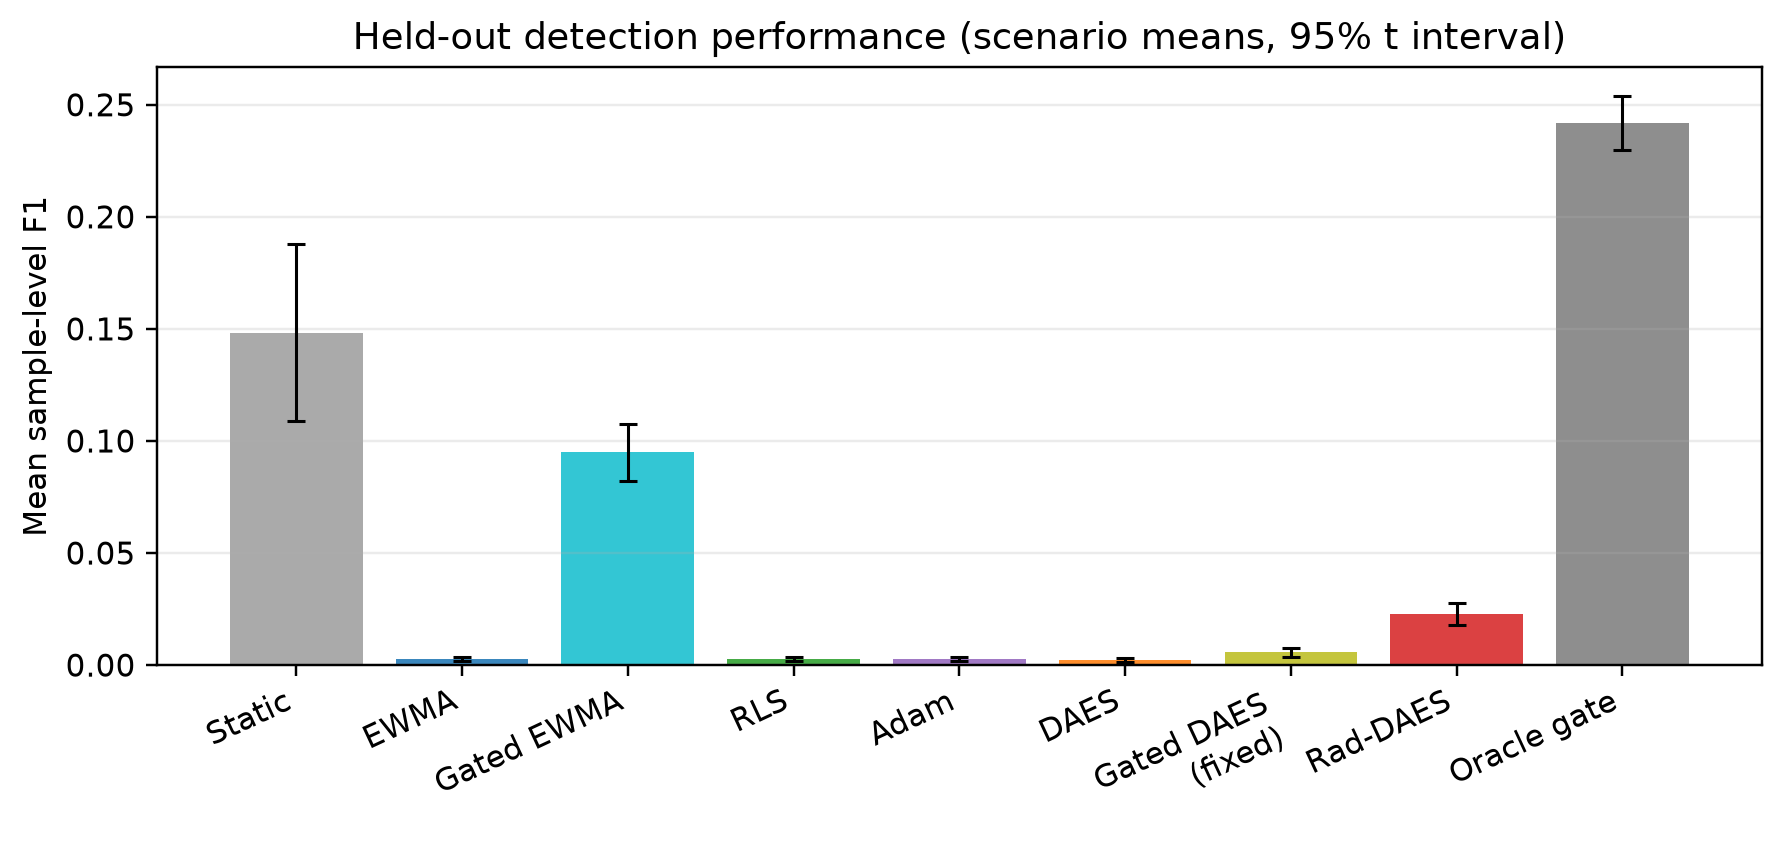
\includegraphics[width=0.92\linewidth]{../results/figures/fig_primary_f1.png}
\caption{Mean sample-level F1 by method. Error bars are 95\% Student-$t$ intervals across the 32 held-out scenario means. The oracle gate is a non-deployable reference.}
\label{fig:primary}
\end{figure}

\paragraph{The operating point dominates the ranking.}
The four methods whose development configurations satisfied the false-alarm constraint (EWMA, RLS, Adam, ungated DAES) have test F1 at most $0.003$ and detect at most 6\% of source events, with test FAR between 2.0 and 2.5/h. They are, in effect, blind at the calibrated operating point. The methods with visible detection either violate the false-alarm constraint or use labels: gated EWMA reaches F1 \GatedEWMAFone{} at \GatedEWMAFarPerHour{}/h, and Rad-DAES reaches \RadDAESFone{} at \RadDAESFarPerHour{}/h. \texttt{static} reaches \StaticFone{} only by alarming on 13.4\% of all samples. There is no deployable method in the matrix that is both sensitive and quiet. Figure~\ref{fig:tradeoff} plots this trade-off directly.

Table~\ref{tab:discrimination} separates threshold choice from separability. The oracle gate has the highest ROC AUC (0.773) and PR AUC (0.223), followed by \texttt{static} (0.728 and 0.128) and gated EWMA (0.691 and 0.089). Rad-DAES obtains ROC AUC \RadDAESRocAuc{} and PR AUC \RadDAESPrAuc{}, below both gated EWMA and \texttt{static}. The ordering is therefore not an artefact of one threshold: the DAES-based methods rank source samples less well than the simpler alternatives on these streams.

\begin{table}[t]
\centering
\caption{Threshold-free discrimination and gate behaviour. ROC/PR AUC use the pre-update score and do not depend on the alarm threshold. Event detection is the fraction of 960 source events with at least one alarm. Alarm fraction is the fraction of all evaluated samples that alarm. Release rate is the fraction of samples in which the sustained-exceedance release is active.}
\label{tab:discrimination}
\scriptsize
\setlength{\tabcolsep}{3pt}
\begin{tabular}{lccccccc}
\toprule
Method & ROC AUC & PR AUC & Event det. & Alarm frac. & Gate rej.\ clean & Gate rej.\ source & Release rate \\
\midrule
Static & 0.728 & 0.128 & 0.821 & 0.1341 & 0.397 & 0.630 & 0.0017 \\
EWMA & 0.622 & 0.031 & 0.060 & 0.0007 & 0.260 & 0.333 & 0.0000 \\
Gated EWMA & 0.691 & 0.089 & 0.406 & 0.0296 & 0.275 & 0.406 & 0.0000 \\
RLS & 0.622 & 0.031 & 0.060 & 0.0007 & 0.260 & 0.333 & 0.0000 \\
Adam & 0.637 & 0.033 & 0.056 & 0.0007 & 0.260 & 0.333 & 0.0000 \\
DAES & 0.600 & 0.024 & 0.054 & 0.0006 & 0.260 & 0.330 & 0.0000 \\
Gated DAES (fixed) & 0.558 & 0.019 & 0.059 & 0.0019 & 0.260 & 0.326 & 0.0000 \\
Rad-DAES & 0.629 & 0.036 & 0.105 & 0.0054 & 0.261 & 0.338 & 0.0000 \\
Oracle gate & 0.773 & 0.223 & 0.736 & 0.0039 & 0.260 & 0.485 & 0.0000 \\
\bottomrule
\end{tabular}

\end{table}

\begin{figure}[t]
\centering
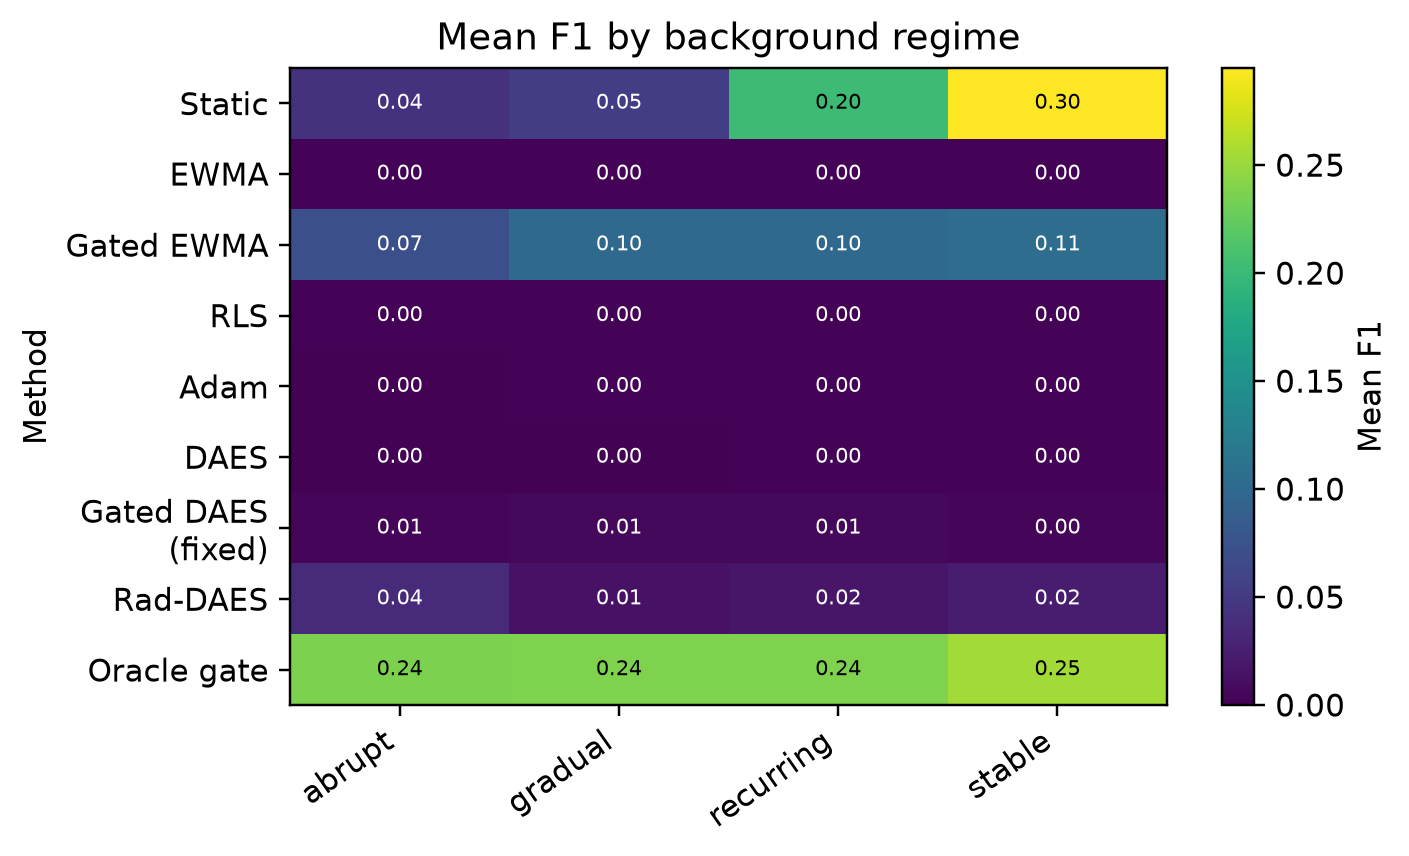
\includegraphics[width=0.92\linewidth]{../results/figures/fig_f1_by_regime.png}
\caption{Mean F1 by background regime. Each cell is the mean over the eight fault conditions and five seeds.}
\label{fig:regime}
\end{figure}

\begin{figure}[t]
\centering
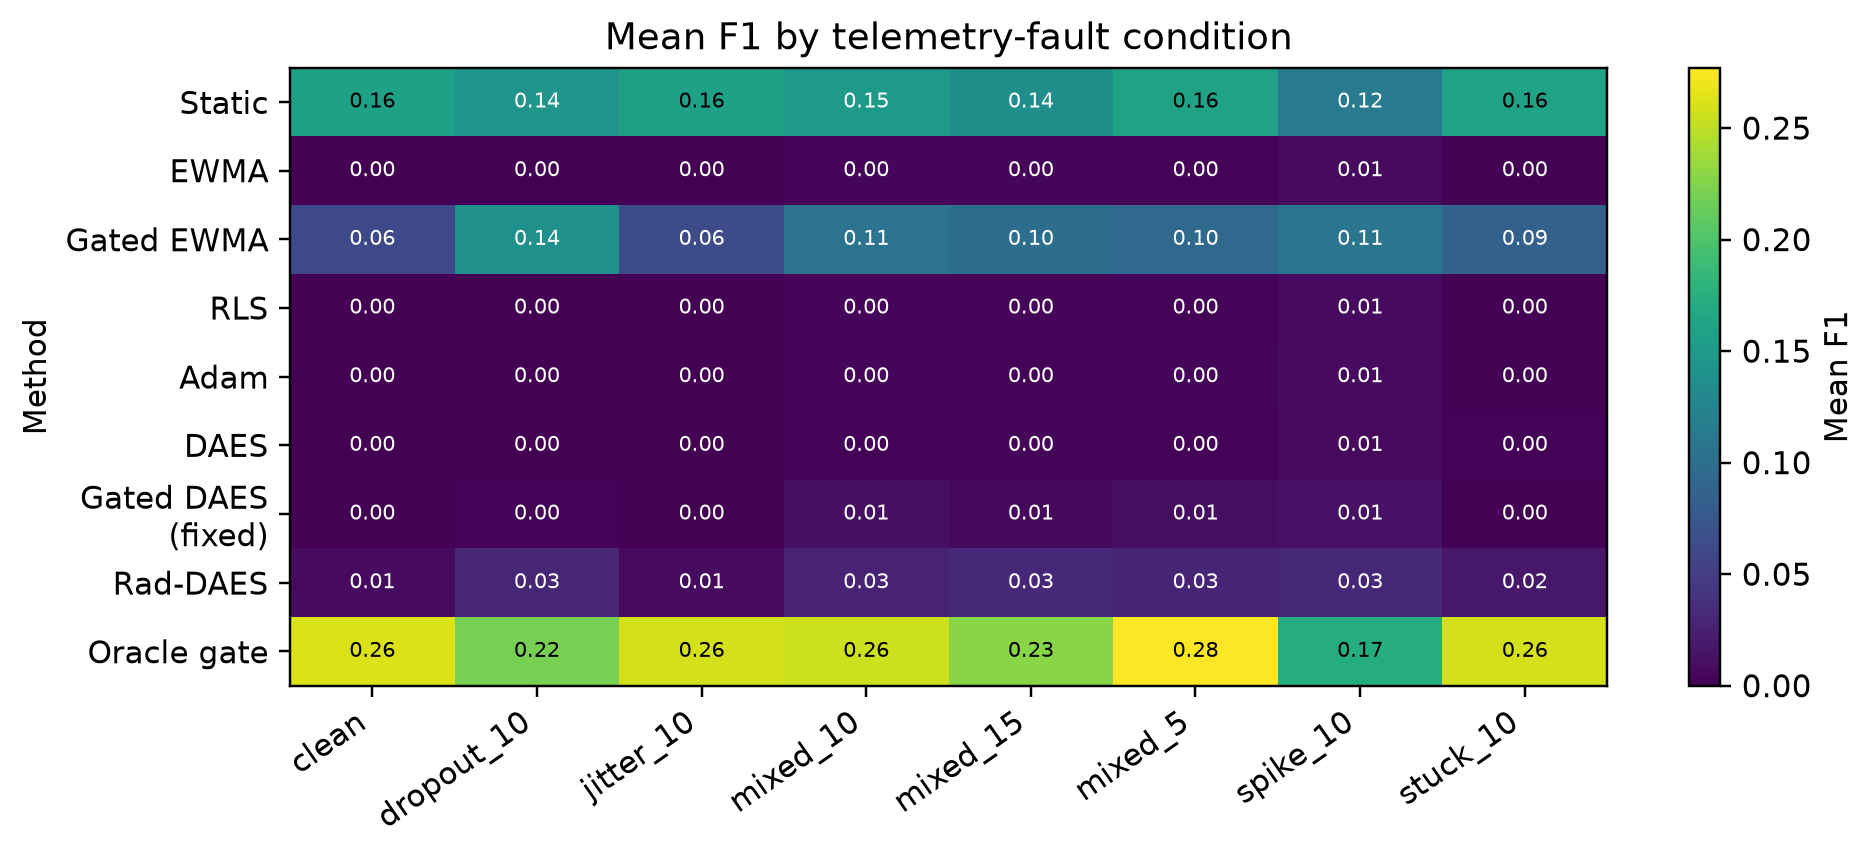
\includegraphics[width=0.98\linewidth]{../results/figures/fig_f1_by_fault.png}
\caption{Mean F1 by telemetry-fault condition. Each cell is the mean over the four regimes and five seeds.}
\label{fig:fault}
\end{figure}

\begin{figure}[t]
\centering
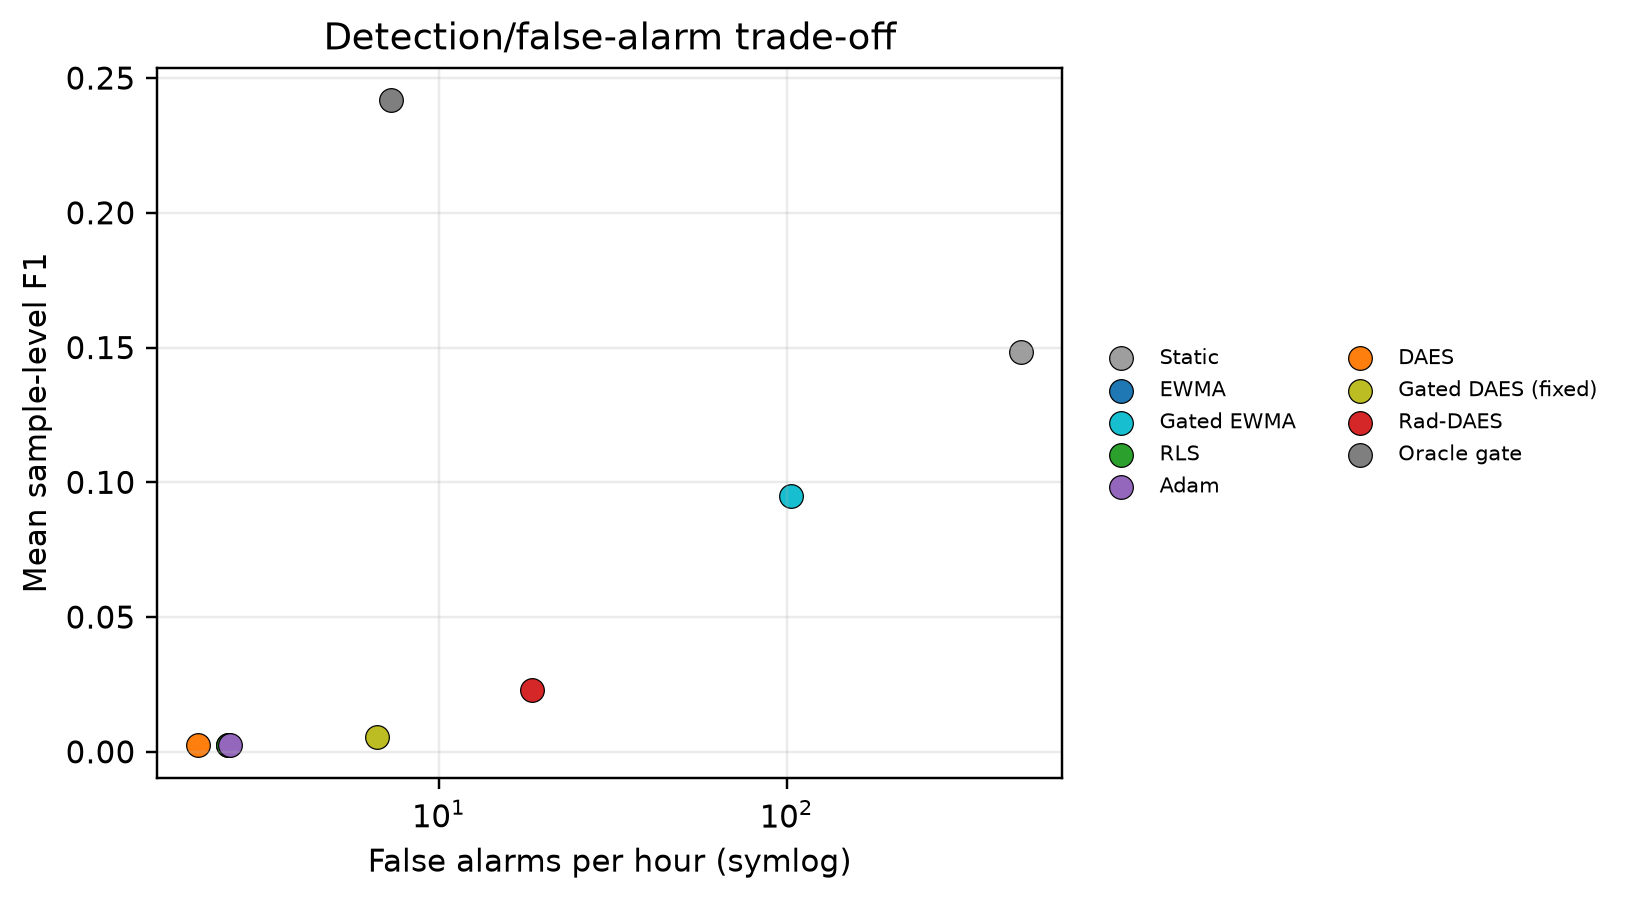
\includegraphics[width=0.78\linewidth]{../results/figures/fig_far_vs_f1.png}
\caption{Detection/false-alarm trade-off. The horizontal axis is symlog because static and some gated configurations produce very large drift-induced false-alarm burdens.}
\label{fig:tradeoff}
\end{figure}

\paragraph{Regime and fault structure.}
Figures~\ref{fig:regime} and~\ref{fig:fault} show that performance is not uniform. The recurring regime is the only regime not used for tuning; it is therefore the clearest check of whether a configuration generalises to a different drift shape. It does not rescue the candidate: Rad-DAES remains below gated EWMA and far below the oracle. Fault conditions change which samples are eligible for updating, so a method that looks adequate on clean streams can lose when dropout, jitter, stuck, or spike faults are present. The spike condition is the worst for false alarms: Rad-DAES reaches \RadDAESFarPerHour{}/h on average but 68.8/h under \texttt{spike\_10}, because a spike both alarms and freezes the update.

\paragraph{Gate behaviour.}
The gate rejects 26.1\% of clean samples and 33.8\% of source samples for Rad-DAES, and the sustained release is active on about $3\times10^{-6}$ of samples. The release is not merely rare: in the representative trace (Figure~\ref{fig:trace}) the consecutive-exceedance counter reaches 89 samples and then resets, one sample short of the 90-sample patience, so the model stays frozen through the step. The tracked mean remains near its pre-step value for roughly 350\,s while the true background has already moved by about 170 counts/s. The gate's source-rejection rate is the expected cost of protecting the background, but here the same mechanism also protects the background from the drift it is supposed to follow. Figure~\ref{fig:gate} summarises the rejection rates by sample type.

\begin{figure}[t]
\centering
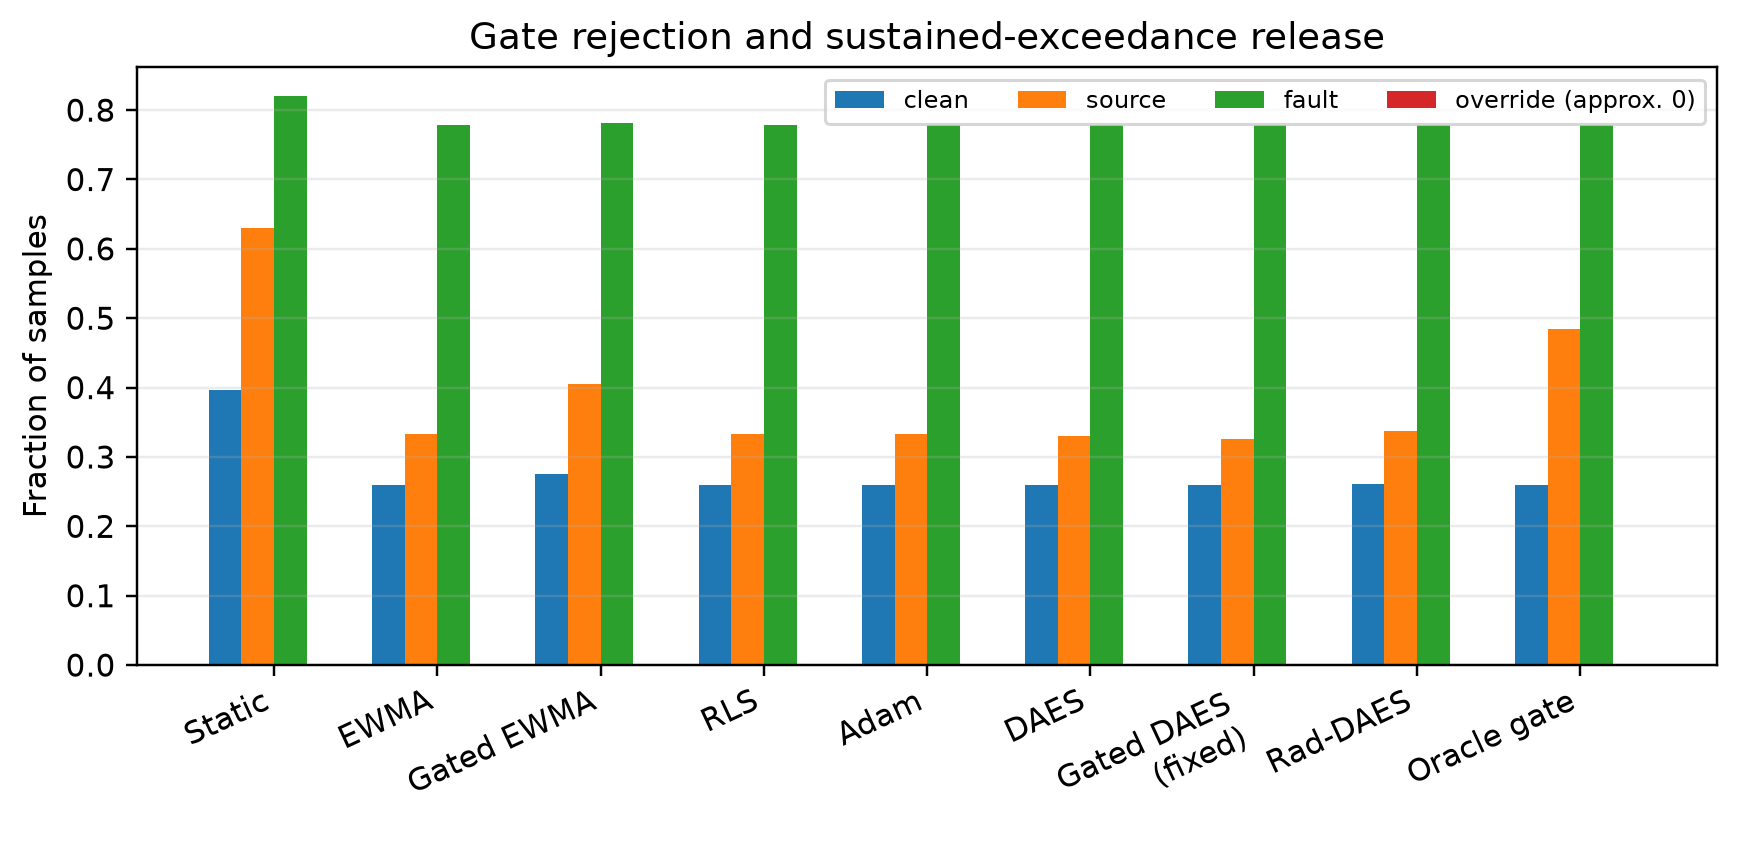
\includegraphics[width=0.92\linewidth]{../results/figures/fig_gate.png}
\caption{Gate rejection rates for clean, source, and fault samples, and the rate of sustained-exceedance release. A high source-rejection rate is the expected cost of protecting the background; it is also a recall risk.}
\label{fig:gate}
\end{figure}

\begin{figure}[t]
\centering
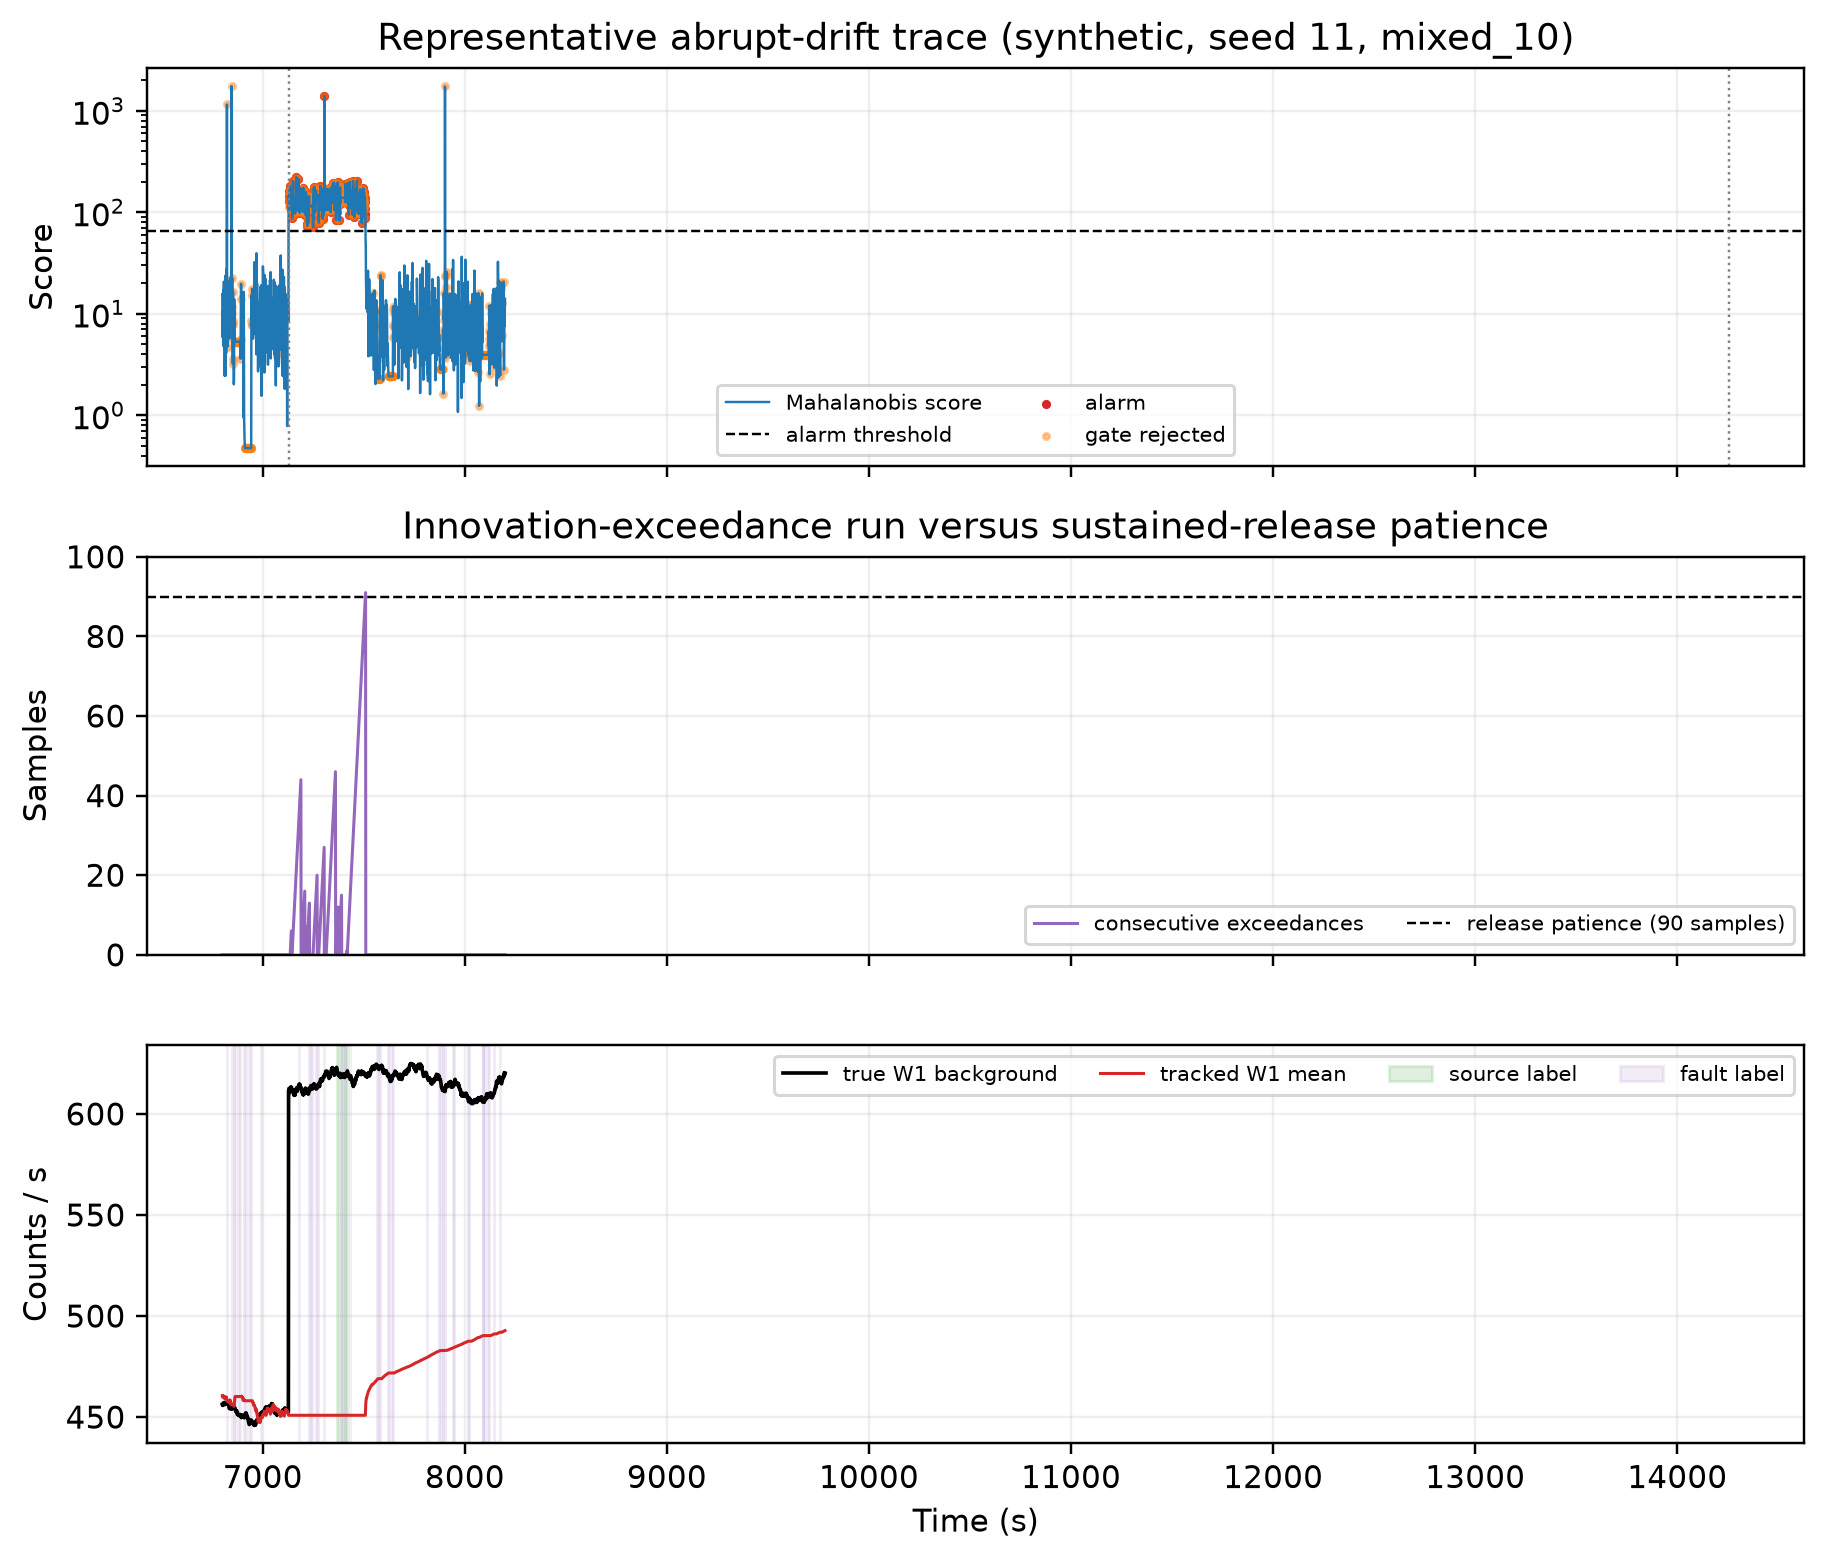
\includegraphics[width=0.95\linewidth]{../results/figures/fig_trace.png}
\caption{Representative abrupt-drift trace for Rad-DAES (synthetic, seed 11, \texttt{mixed\_10}). Top: pre-update score, alarms, and gate rejections. Middle: consecutive innovation exceedances versus the 90-sample release patience; the counter peaks at 89 and resets. Bottom: true and tracked W1 background, with source and fault labels.}
\label{fig:trace}
\end{figure}

\paragraph{Recovery and stability.}
Figure~\ref{fig:recovery} reports recovery time after abrupt steps. Recovery is defined as the first sample at which every window's relative mean error stays below 5\% for 30 consecutive samples; an event that never meets the condition is not silently counted as a success. Rad-DAES recovers 55 of 80 abrupt-step events with a mean recovery time of \RadDAESRecoveryMean{}\,s; gated EWMA recovers all 80 at \GatedEWMARecoveryMean{}\,s but with a much higher false-alarm burden; ungated EWMA and RLS recover all 80 at about 399\,s while remaining nearly blind to sources; \texttt{static} recovers none. Recovery and detection therefore pull in opposite directions in this matrix, and no method achieves both.

\begin{figure}[t]
\centering
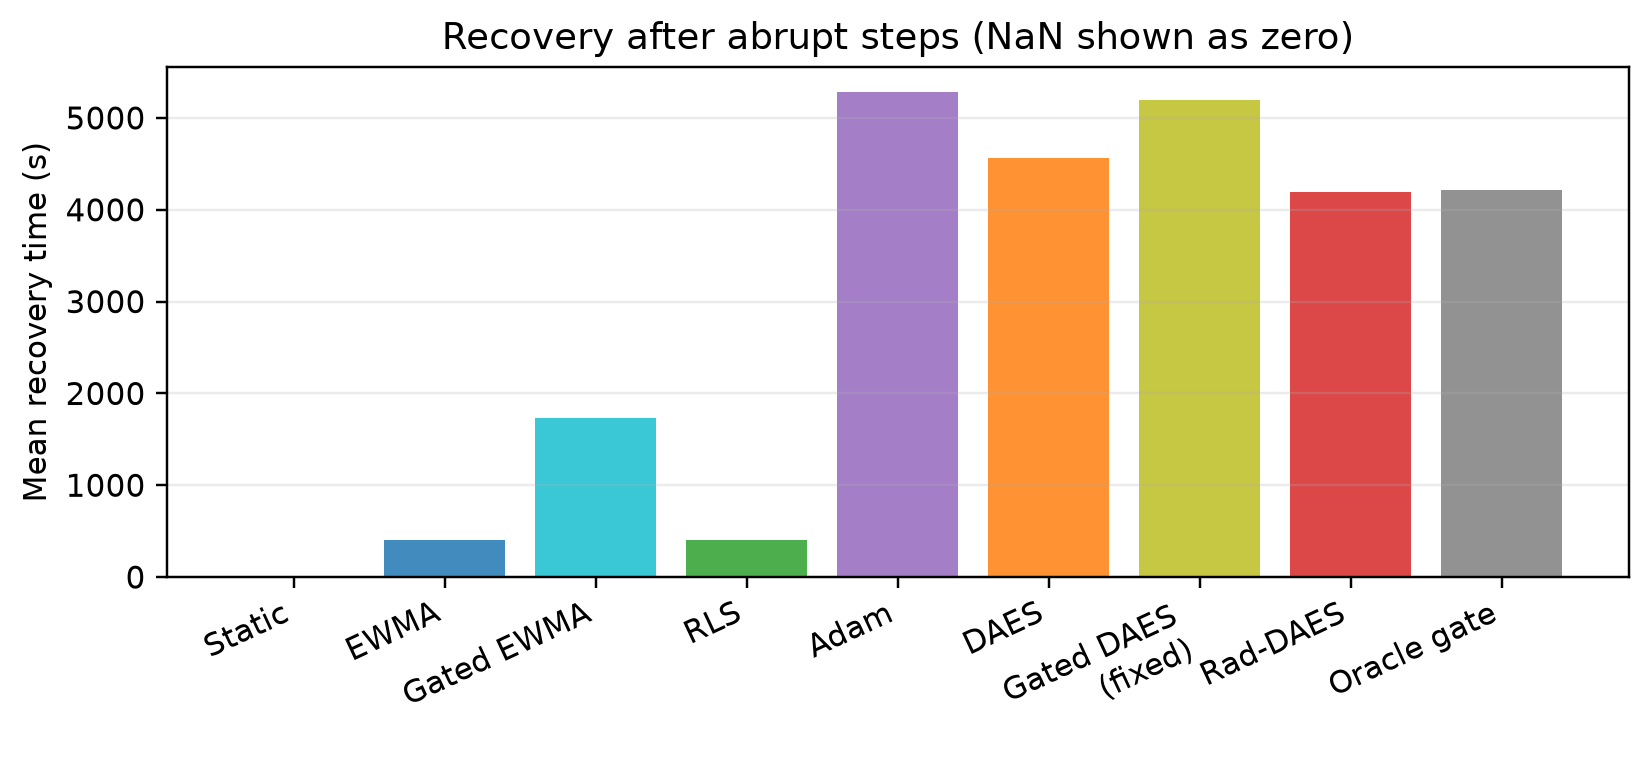
\includegraphics[width=0.78\linewidth]{../results/figures/fig_recovery.png}
\caption{Mean recovery time after abrupt steps. Missing values are shown as zero only for display; they are not treated as recovered in the tables.}
\label{fig:recovery}
\end{figure}

\begin{table}[t]
\centering
\caption{Paired differences (Rad-DAES minus the named method) over matched scenario/seed pairs. Each pair is one held-out run; the 160 pairs are 32 scenarios $\times$ 5 seeds, and the five seeds of a scenario are treated as independent observations, so within-scenario clustering is not modelled. Positive F1 is better; positive FAR and BG are worse. Intervals are descriptive 95\% Student-$t$ intervals and are not multiplicity-corrected.}
\label{tab:paired}
\scriptsize
\begin{tabular}{llccc}
\toprule
Comparison & Metric & Mean difference & 95\% CI & Pairs \\
\midrule
Rad-DAES minus Static & f1 & -0.125 & [-0.146, -0.105] & 160 \\
Rad-DAES minus Static & far\_per\_hour & -453.9 & [-534.8, -372.9] & 160 \\
Rad-DAES minus Static & bg\_rel\_error & -0.029 & [-0.034, -0.024] & 160 \\
Rad-DAES minus EWMA & f1 & 0.020 & [0.013, 0.027] & 160 \\
Rad-DAES minus EWMA & far\_per\_hour & 16.032 & [6.324, 25.741] & 160 \\
Rad-DAES minus EWMA & bg\_rel\_error & 0.010 & [0.008, 0.012] & 160 \\
Rad-DAES minus Gated EWMA & f1 & -0.072 & [-0.081, -0.063] & 160 \\
Rad-DAES minus Gated EWMA & far\_per\_hour & -84.240 & [-122.8, -45.653] & 160 \\
Rad-DAES minus Gated EWMA & bg\_rel\_error & 0.008 & [0.006, 0.010] & 160 \\
Rad-DAES minus RLS & f1 & 0.020 & [0.013, 0.027] & 160 \\
Rad-DAES minus RLS & far\_per\_hour & 16.032 & [6.324, 25.741] & 160 \\
Rad-DAES minus RLS & bg\_rel\_error & 0.010 & [0.008, 0.012] & 160 \\
Rad-DAES minus Adam & f1 & 0.020 & [0.014, 0.027] & 160 \\
Rad-DAES minus Adam & far\_per\_hour & 16.008 & [6.291, 25.726] & 160 \\
Rad-DAES minus Adam & bg\_rel\_error & -0.002 & [-0.004, -0.000] & 160 \\
Rad-DAES minus DAES & f1 & 0.020 & [0.014, 0.027] & 160 \\
Rad-DAES minus DAES & far\_per\_hour & 16.478 & [6.720, 26.236] & 160 \\
Rad-DAES minus DAES & bg\_rel\_error & -0.012 & [-0.017, -0.007] & 160 \\
Rad-DAES minus Gated DAES (fixed) & f1 & 0.017 & [0.011, 0.023] & 160 \\
Rad-DAES minus Gated DAES (fixed) & far\_per\_hour & 11.860 & [2.278, 21.441] & 160 \\
Rad-DAES minus Gated DAES (fixed) & bg\_rel\_error & -0.043 & [-0.044, -0.043] & 160 \\
Rad-DAES minus Oracle gate & f1 & -0.219 & [-0.231, -0.207] & 160 \\
Rad-DAES minus Oracle gate & far\_per\_hour & 11.217 & [1.634, 20.799] & 160 \\
Rad-DAES minus Oracle gate & bg\_rel\_error & 0.011 & [0.010, 0.012] & 160 \\
\bottomrule
\end{tabular}

\end{table}

\paragraph{Tuning and fallbacks.}
Table~\ref{tab:tuning} records the selected development configuration for each method. Four of the nine methods used a fallback, meaning that no candidate met both the background-error and false-alarm constraints on the development scenarios. Rad-DAES selected the largest gain in the grid ($\gamma=0.5$) with a development FAR of 28.6/h, more than fourteen times the constraint; gated EWMA selected the smallest EWMA weight but still had a development FAR of 99.4/h. The oracle gate selected the smallest gain ($\gamma=0.05$) and had a development FAR of 12.5/h. The oracle's advantage is therefore not an isolated gate effect: it combines perfect labelling with a ten-fold gentler step, and the two cannot be separated in this matrix. The selected configurations were frozen before the test matrix.

\begin{table}[t]
\centering
\caption{Selected development configurations and development means. ``Fallback'' means no candidate satisfied both the background-error and false-alarm constraints.}
\label{tab:tuning}
\scriptsize
\begin{tabular}{llcccc}
\toprule
Method & Selected configuration & Status & Dev F1 & Dev BG & Dev FAR/h \\
\midrule
Static & \texttt{default} & fixed & 0.137 & 0.0644 & 647.7 \\
EWMA & \texttt{ewma\_alpha=0.02} & feasible & 0.004 & 0.0136 & 1.11 \\
Gated EWMA & \texttt{ewma\_alpha=0.005;gate\_quantile=0.999} & fallback & 0.078 & 0.0148 & 99.36 \\
RLS & \texttt{rls\_forgetting=0.98} & feasible & 0.004 & 0.0136 & 1.11 \\
Adam & \texttt{adam\_learning\_rate=0.02} & feasible & 0.005 & 0.0261 & 1.09 \\
DAES & \texttt{daes\_gain=0.2} & feasible & 0.004 & 0.0417 & 1.05 \\
Gated DAES (fixed) & \texttt{daes\_gain=0.5;gate\_quantile=0.995} & fallback & 0.011 & 0.0692 & 12.42 \\
Rad-DAES & \texttt{daes\_gain=0.5;gate\_quantile=0.999} & fallback & 0.036 & 0.0257 & 28.64 \\
Oracle gate & \texttt{daes\_gain=0.05} & fallback & 0.228 & 0.0147 & 12.48 \\
\bottomrule
\end{tabular}

\end{table}

\section{Discussion}

The experiment was designed to test a trade-off, not to demonstrate that a new method wins. The answer is negative, and three mechanisms explain most of it.

\emph{First, the innovation guard confuses drift with a source.} A persistent background step produces a sustained score above the gate threshold, so the gate freezes the mean precisely when the mean needs to move. The 90-sample release was intended to break this deadlock, but it requires an uninterrupted run of exceedances; Poisson noise and the oscillating score reset the counter. In the representative trace the counter peaks at 89 and resets. The result is a frozen model, a long alarm burst, and a slow recovery. This is a design failure of the release rule, not a tuning issue: the rule is brittle by construction because it depends on a run length in a noisy sequence.

\emph{Second, the adaptive background appears to absorb source energy.} Both the mean and the covariance update on a 50-sample time constant, comparable to the 20--60\,s source duration. During the ramp of a source event the score is still below the gate threshold, so the gate passes those samples; the mean then moves toward the source and the covariance learns its outer product, and the score for the peak falls. This is consistent with the threshold-free results: \texttt{static}, which updates neither the mean nor the covariance, has ROC AUC 0.728, while the adaptive methods have ROC AUC between 0.558 and 0.691. We did not run a covariance-frozen or mean-frozen ablation, so the two channels are not separated experimentally; the static-versus-adaptive contrast supports the general mechanism, not the share attributable to covariance. It is the most plausible explanation for why the ungated methods detect only about 6\% of events despite a nominal 3--8$\sigma$ source amplitude.

\emph{Third, the selection rule was infeasible.} The development constraint (FAR $\le 2$/h, background error $\le 0.10$) could not be met by any gated configuration under abrupt drift. The fallback rule then chose configurations that violated the FAR constraint by one to two orders of magnitude, and those configurations were frozen for test. The four feasible methods were feasible only because they were nearly blind. The protocol therefore did not compare methods at a common, achievable operating point; it compared blind methods against noisy ones. A matched-FAR evaluation, or a prespecified ROC/PR analysis, would have been more informative. The ROC/PR table is reported here as a secondary analysis, but it was not the basis of the selection rule.

The practical implication is that the three decisions should not share one score. A drift detector, a source detector, and a telemetry-integrity check answer different questions \citep{gama2014survey,isermann2005model}; using the same Mahalanobis score for gating and alarming creates the coupling observed here. A two-timescale covariance (fast for the mean, slow or robust for the detector), or a covariance that is frozen during suspected sources, is a concrete next step. None of these is implemented or validated in this draft.

The draft does not establish that Rad-DAES is novel. The literature review here is structured but not a full systematic review; the closest related work on portal data and concept drift is cited only to frame the problem. A novelty claim would require a protocol-driven review and a direct comparison on public data.

\section{Limitations and threats to validity}

\begin{itemize}
  \item \textbf{No real data.} RADAI requires an account and a large download; PyRIID requires a compatible Python environment and spectra conversion; the JRC reference spectra are not a continuous portal stream. No credentials were used and no real stream was parsed. Gate~1 of the project plan is a partial failure.
  \item \textbf{Synthetic generator.} The regimes, source templates, amplitudes, and fault rates are design choices. They are not fitted to measured background. The Poisson model ignores detector resolution, dead time, and spectrum unfolding \citep{knoll2010radiation}. The $\sin^2$ source profile makes the peak narrow, which penalises sample-level F1; event-level detection is reported to reduce that sensitivity, but it does not eliminate it. The design is reported in the form recommended for simulation studies \citep{morris2019simulation}, but a synthetic study cannot substitute for measured streams.
  \item \textbf{Mechanism inferred, not isolated.} The adaptive-background explanation (mean and covariance) is supported by the static-versus-adaptive contrast and by the saved traces, but no covariance-frozen or mean-frozen ablation was run, so the two channels are not separated. The gate-deadlock explanation is directly visible in one representative trace; the 89-versus-90 near miss is illustrative, not a distributional estimate.
  \item \textbf{Small seed budget.} Five seeds were evaluated per scenario. The primary 95\% confidence intervals are calculated across the 32 scenario means after averaging the five seeds within each scenario. These intervals are descriptive and conditional on the fixed scenario design. They do not quantify uncertainty beyond the selected scenarios or account for model misspecification \citep{greenland2016statistical}.
  \item \textbf{No multiplicity correction.} The scenario-level and paired comparisons are descriptive. A claim of statistical significance is not made, and no false-discovery-rate procedure is applied \citep{benjamini1995controlling}.
  \item \textbf{Design choices.} The 90-sample (90\,s) release, the 0.5--1.5\,s timing bound, the 0.25--3.5 Fano bounds, the 0.25 covariance floor, the 50-sample covariance time constant, and the six windows are choices, not validated constants. Sensitivity analyses are future work.
  \item \textbf{Threshold transfer.} Thresholds calibrated on clean stable streams do not transfer to drift regimes: even the oracle gate has 7.3 false alarms/h on test. The 1/h calibration target is therefore not an operational guarantee, and portal false-alarm testing requires a broader operating-characteristic study than the one reported here \citep{burr2007alarm,leber2020false}.
  \item \textbf{DAES provenance.} The DAES equations follow the supplied scalar reference implementation. The matrix update in some generated planning material is not implemented as DAES. The wrapper's use of a Gaussian quasi-likelihood Hessian is an adaptation, not a theorem.
  \item \textbf{No field readiness.} Runtime is offline Python on synthetic arrays. No hardware latency, network delay, calibration uncertainty, or regulatory requirement is modelled.
\end{itemize}

\section{Reproducibility}

{\sloppy
The repository is self-contained and separate from the unrelated projects that share the workspace. The synthetic generator, gate, DAES controller, background model, detector, runner, tests, scripts, raw CSV files, tables, and figures are included. The packaging follows the reproducibility principle that data, code, and the computational narrative should be inspectable together \citep{peng2011reproducible}. The main commands are:\par}
\begin{verbatim}
python -m pip install -e .
python -m pytest -q
python scripts/run_benchmarks.py --mode full --output results/raw
python scripts/aggregate_results.py
python scripts/make_figures.py
python scripts/audit_results.py
\end{verbatim}
The runner writes a manifest with Python and package versions, configuration hashes, seed lists, and run counts. Every table and figure is generated from saved CSV or trace files; no result is typed into the manuscript by hand. The audit script checks matrix completeness, the frozen selection and thresholds, a determinism spot-check of saved rows, config hashes, and the presence of every table, figure, and macro used here. The original DAES reference file was read from an external snapshot for interface documentation and was not vendored or modified. Its SHA-256 and the archive SHA-256 are recorded in \texttt{docs/daes\_interface.md}.

{\sloppy
The raw run was launched with \texttt{--output results} and then moved into \texttt{results/raw/} to match the layout read by the aggregation and audit scripts; the only edited field was the trace-path column of \texttt{trace\_index.csv}. This is documented in \texttt{results/raw/README.md}.\par}

\section{Conclusion}

This draft delivers a small, complete, reproducible synthetic study of guarded drift-aware background tracking, and its result is negative. Rad-DAES does not improve the detection/false-alarm trade-off on these streams: its F1 is \RadDAESFone{} at \RadDAESFarPerHour{}/h, while the four false-alarm-compliant methods are nearly blind and the non-deployable oracle reaches only \BestValue{}. The traces identify two concrete failure modes, gate-induced freezing under drift and apparent adaptive-background contamination during source ramps, and the development selection rule is shown to be infeasible at the prespecified operating point. The value of the draft is the auditable pipeline and the explicit evidence boundary, not a claim that the candidate method is ready for a portal.

\bibliographystyle{plainnat}
\bibliography{references}

\appendix
\section{Implementation map}

\begin{table}[htbp]
\centering
\caption{Where each component is implemented and tested. Package paths are relative to \texttt{src/rad\_daes/}; script, test, and report paths are relative to the repository root.}
\small
\setlength{\tabcolsep}{4pt}
\begin{tabular}{lll}
\toprule
Component & Source & Test \\
\midrule
Synthetic streams & \texttt{data/synthetic.py} & \texttt{tests/test\_synthetic.py} \\
Window definitions & \texttt{preprocessing/windows.py} & configuration checks \\
Background model & \texttt{background/model.py} & \texttt{tests/test\_background.py} \\
Telemetry gate & \texttt{telemetry/gate.py} & \texttt{tests/test\_gate.py} \\
DAES controller & \texttt{adaptation/daes.py} & \texttt{tests/test\_daes.py} \\
Detector & \texttt{detection/detector.py} & runner integration \\
Metrics & \texttt{evaluation/metrics.py} & \texttt{tests/test\_metrics.py} \\
Runner and calibration & \texttt{evaluation/runner.py} & \texttt{tests/test\_runner.py} \\
Aggregation & \texttt{scripts/aggregate\_results.py} & table checks \\
Audit & \texttt{scripts/audit\_results.py} & \texttt{results/audit\_report.md} \\
\bottomrule
\end{tabular}
\end{table}

\section{Protocol revisions}

The source-placement bug, the sustained-exceedance release, the covariance floor, and the midpoint source profile were fixed on 28 October 2026 before the held-out matrix was run. The revision log is in \texttt{docs/protocol.md}. No held-out result was inspected before these changes. After the frozen test matrix was complete, the threshold-free ROC/PR table and the event-level detection summary were added as secondary analyses; they are computed from columns already saved by the frozen run, and the primary estimand and selection rule were not changed.

\clearpage
\section{Artifact inventory}

Table~\ref{tab:artifacts} lists the paths a reader needs in order to inspect or rerun the study. Counts describe the working repository of 28 October 2026 and exclude Python caches and \LaTeX{} build byproducts; the submission mirror differs only in that the cover-letter DOCX sits at the bundle root, so its \texttt{paper/} directory has six files.

\begin{table}[htbp]
\centering
\caption{Frozen artifact inventory. File counts exclude \texttt{\_\_pycache\_\_} directories.}
\label{tab:artifacts}
\small
\setlength{\tabcolsep}{4pt}
\begin{tabular}{llr}
\toprule
Path & Contents & Files \\
\midrule
\texttt{src/rad\_daes/} & Generator, gate, DAES controller, model, detector, metrics, runner & 16 \\
\texttt{configs/} & Data, model, and experiment configuration & 3 \\
\texttt{tests/} & Unit and integration tests (44 passing) & 7 \\
\texttt{results/raw/} & Calibration, development, and test CSVs; manifest; 4 traces & 13 \\
\texttt{results/tables/} & CSV, \LaTeX{} tables, and generated macros & 16 \\
\texttt{results/figures/} & Seven PNG figures & 7 \\
\texttt{docs/} & Protocol, decisions, DAES interface, results summary, checklist & 8 \\
\texttt{paper/} & Manuscript source, PDF, cover letter, bibliography, supplementary note & 7 \\
\bottomrule
\end{tabular}
\end{table}

The primary test artifact is \texttt{results/raw/test\_runs.csv} (1{,}440 rows). The audit report is regenerated by \texttt{scripts/audit\_results.py} and records 22 checks. No real radiation data are included, because none were obtained (Section~6).

\end{document}
